\chapter{Génération, simulation et reconstruction des événements} \label{chap:reco}

Afin d'être en mesure de confronter les prédictions théoriques aux données expérimentales, il faut être capable de simuler la réponse du détecteur pour un processus donné. Pour cela, il faut tout d'abord simuler une collision entre deux protons comme si elle avait vraiment eut lieu au LHC. On utilise pour cela des outils développés spécifiquement pour cet usage, appelés générateurs d'événements Monte Carlo (MC), qui permettent de simuler l'interaction entre deux partons et de générer toutes les particules créées lors de la collision. Il est ensuite nécessaire de simuler l'interaction de ces particules avec le détecteur, afin d'extraire les réponses des différents sous-détecteurs. Ces différentes étapes sont traitées dans ce chapitre., en commençant par une description succincte des processus de génération et de simulation. La majeure partie de ce chapitre sera consacrée à la description des algorithmes de reconstruction des particules, cruciaux pour les analyses de physique.

\section{Génération des événements}

\fxerror{Compléter cette partie - 1 ou 2 pages de plus}

%Afin d'extraire des informations sur les observables physiques, telles que les sections efficaces par exemple, on utilise un développement perturbatif. En effet, la probabilité de transition d'un état initial $\ket{i}$ à un état final $\ket{f}$ est calculée en utilisant la règle d'or de Fermi. Cette règle est obtenue grâce à la théorie des perturbations, en considérant que le temps nécessaire à l'interaction est bien plus petit que le temps nécessaire à l'observation.

%La précision du résultat dépend de l'ordre du calcul. Le premier ordre, celui le plus simple à calculer, correspond à un nombre de vertex de 2, et est appelé calcul à l'arbre (ou \emph{LO}, pour \emph{Leading Order}).

\subsection{L'événement dur}

Lors d'une collision entre deux protons, seul les constituants (les partons: quarks et gluons) vont interagir, chacun emportant une certaine fraction $x$ de l'impulsion totale du proton incident. Afin d'extraire des informations sur les observables physiques, telles que les sections efficaces par exemple, on utilise un développement perturbatif à plusieurs ordres.

L'événement dur est décrit de façon analytique en utilisant ce développement perturbatif. Le générateur détermine grâce à un ensemble de règles, appelées règles de Feynman, la matrice de transition entre l'état initial et l'état final. Le calcul au premier ordre (LO, \emph{Leading Order}) est disponible pour les processus les plus importants du Modèle Standard, implémenté dans des programmes tels que \texttt{MADGRAPH} \citep{madgraph} par exemple. Les simulations aux ordres supérieurs deviennent extrêmement complexes et sont disponibles seulement pour un petit nombre de processus et ont été implémenté dans des programmes particuliers comme \texttt{POWHEG} \citep{Alioli:2010xd}, \texttt{MC@NLO} \citep{1126-6708-2002-06-029}, etc.

La section efficace partonique $\sigma_{ij} \rightarrow X$, avec $i, j = \Pgluon, \Pquark$ et $X$ un état final choisi, peut s'exprimer de la façon suivante :
\begin{align}
  \sigma_{X} &= \sum_{ij} \int \displaylimits_0^1 \int \displaylimits_0^1 f_i\left( x_i, \mu^2 \right) f_j\left(x_j, \mu^2\right) \sigma_{ij \rightarrow X}\, \mathrm{d}x_i \mathrm{d}x_j \notag \\
  \sigma_{ij \rightarrow X} &\propto \int \prod \displaylimits_{k = 1}^{N} \frac{\mathrm{d}^3p_k}{\left( 2 \pi \right)^2 2 E_k} \delta^4\left( p_i + p_j - \sum_{k = 1}^{N} p_k \right) \left| \mathcal{M}_{fi} \right|^2 \label{eq:section_efficace}
\end{align}
où $f_{i, j}$ est la densité de probabilité partonique (détaillée \cref{sec:pdf}), $x_i$ la fraction d'impulsion emportée par le parton $i$, $\mu^2$ l'échelle d'énergie du processus et $\mathcal{M}_{fi}$ l'élément de matrice de transition entre l'état initial $i$ et l'état final $f$. L'élément de matrice est calculé jusqu'à un ordre donné, limité par l'ordre auquel les calculs théoriques ont pu être menés, et l'intégration est effectuée numériquement selon une méthode d'intégration Monte Carlo.

\begin{figure}[tbp]
    \centering
    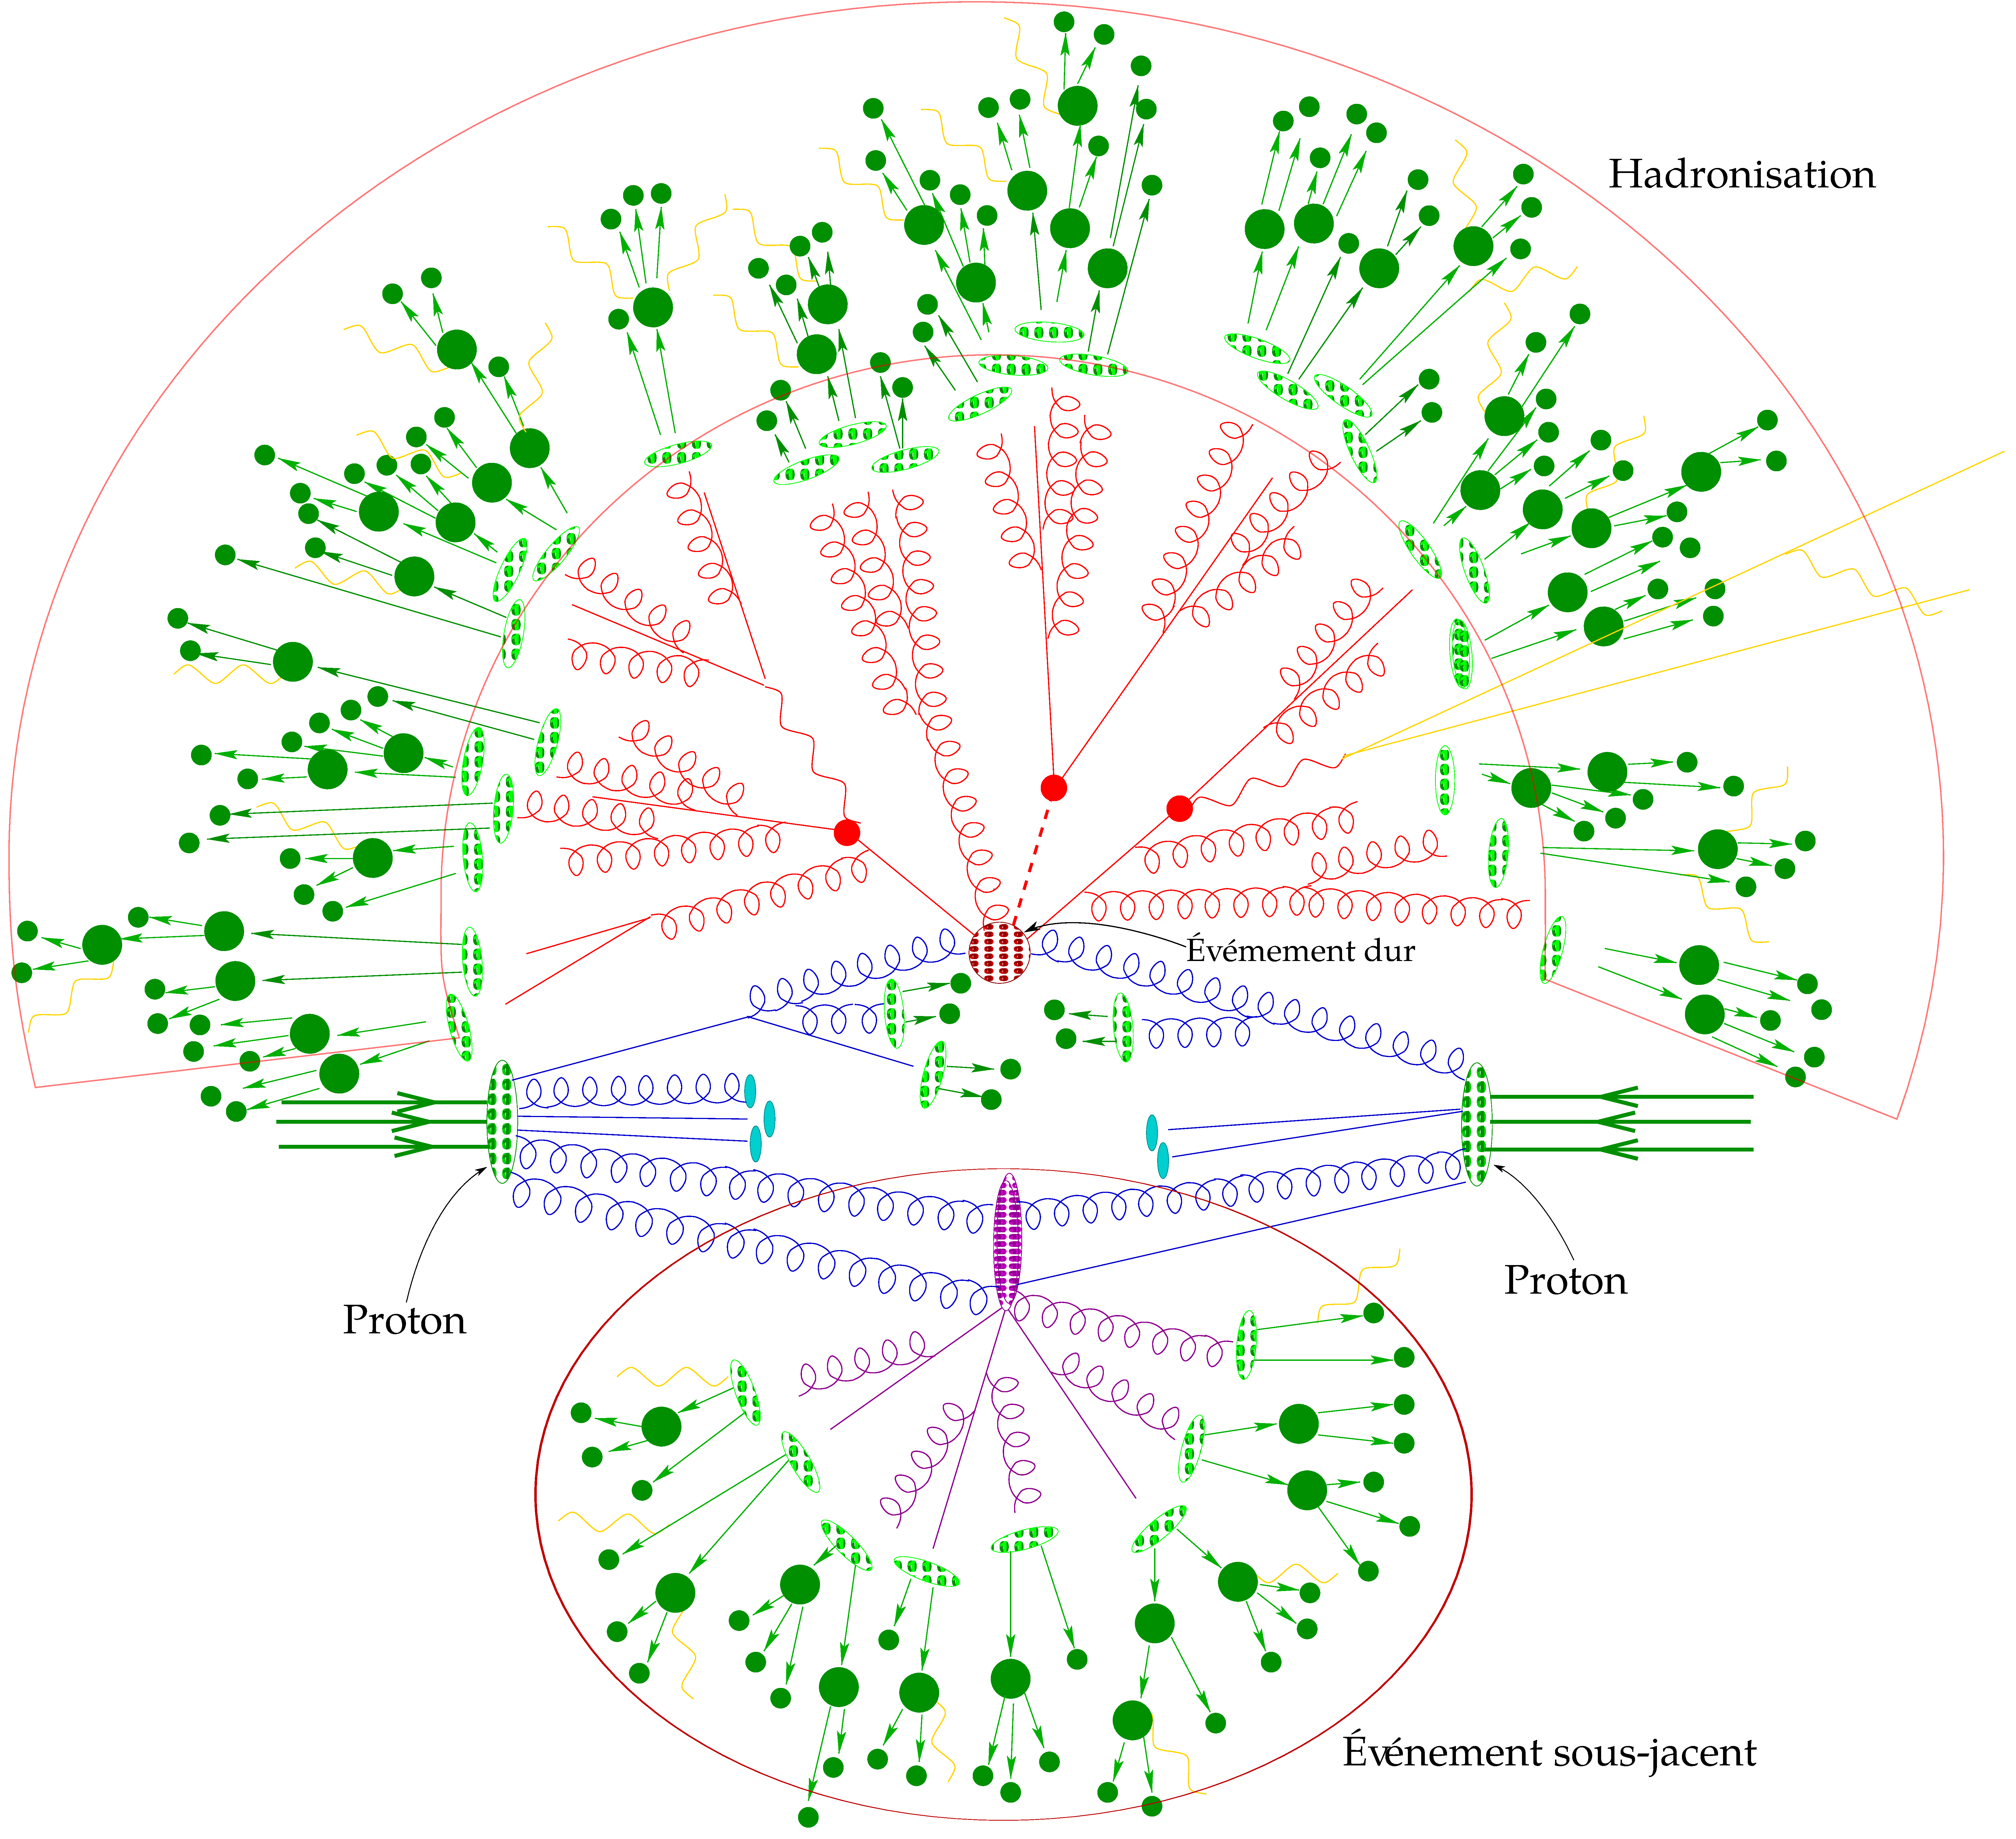
\includegraphics[width=0.99\textwidth]{chapitre3/figs/parton_shower_legend.pdf}
    \caption{Représentation graphique d'une collision de deux protons simulée à l'aide d'un générateur. L'événement dur (au centre, en rouge) est produit par l'interaction de deux partons. Les trois particules produites (rond rouge plein) se désintègrent. C'est à ce niveau qu'intervient l'hadronisation. Des radiations de photons (jaune) ont été rajoutées à chaque étape.}
    \label{fig:parton_shower}
\end{figure}

On obtient en sortie du générateur le quadrivecteur impulsion de chaque particule produite lors de l'événement dur.

\subsection{Densité de probabilité partonique (PDF)} \label{sec:pdf}

Le calcul des sections efficaces des processus faisant intervenir des hadrons nécessite la connaissance des densités de probabilité partonique (PDF) $f_i\left( x, \mu^2 \right)$, qui représente la probabilité de trouver un parton $i$ au sein du hadron, emportant une fraction d'impulsion $x$ lors d'un processus à l'échelle d'énergie $\mu^2$. Ces fonctions ne peuvent pas être déterminées par des calculs perturbatifs, mais sont obtenus à partir d'ajustement des données expérimentales. Les principales sources de données proviennent des mesures de l'expérience HERA, permettant de sonder la structure du proton en faisant collisionner des protons avec des électrons. L'étude de la production des jets au Tevatron et au LHC contribue également considérablement à la connaissance des PDFs des gluons. Malheureusement, l'échelle d'énergie du LHC permet d'obtenir des collisions à très petit $x$ et très grand $\mu^2$, gamme non couverte par les données expérimentales : il est nécessaire d'extrapoler les PDFs, augmentant ainsi les incertitudes liées aux PDFs.

\smallskip

Deux groupes principaux fournissent les PDFs, CTEQ \citep{Owens:2012bv} et MSTW \citep{Martin:2009iq}, qui publient régulièrement des nouvelles PDFs tenant compte des dernières mesures. La \cref{fig:cj12} présente les PDFs pour divers partons issues du jeu de PDFs CJ12, pour une échelle en énergie $\mu^2 = \SI{100}{\GeV}$.

\begin{figure}[tbp]
  \centering
  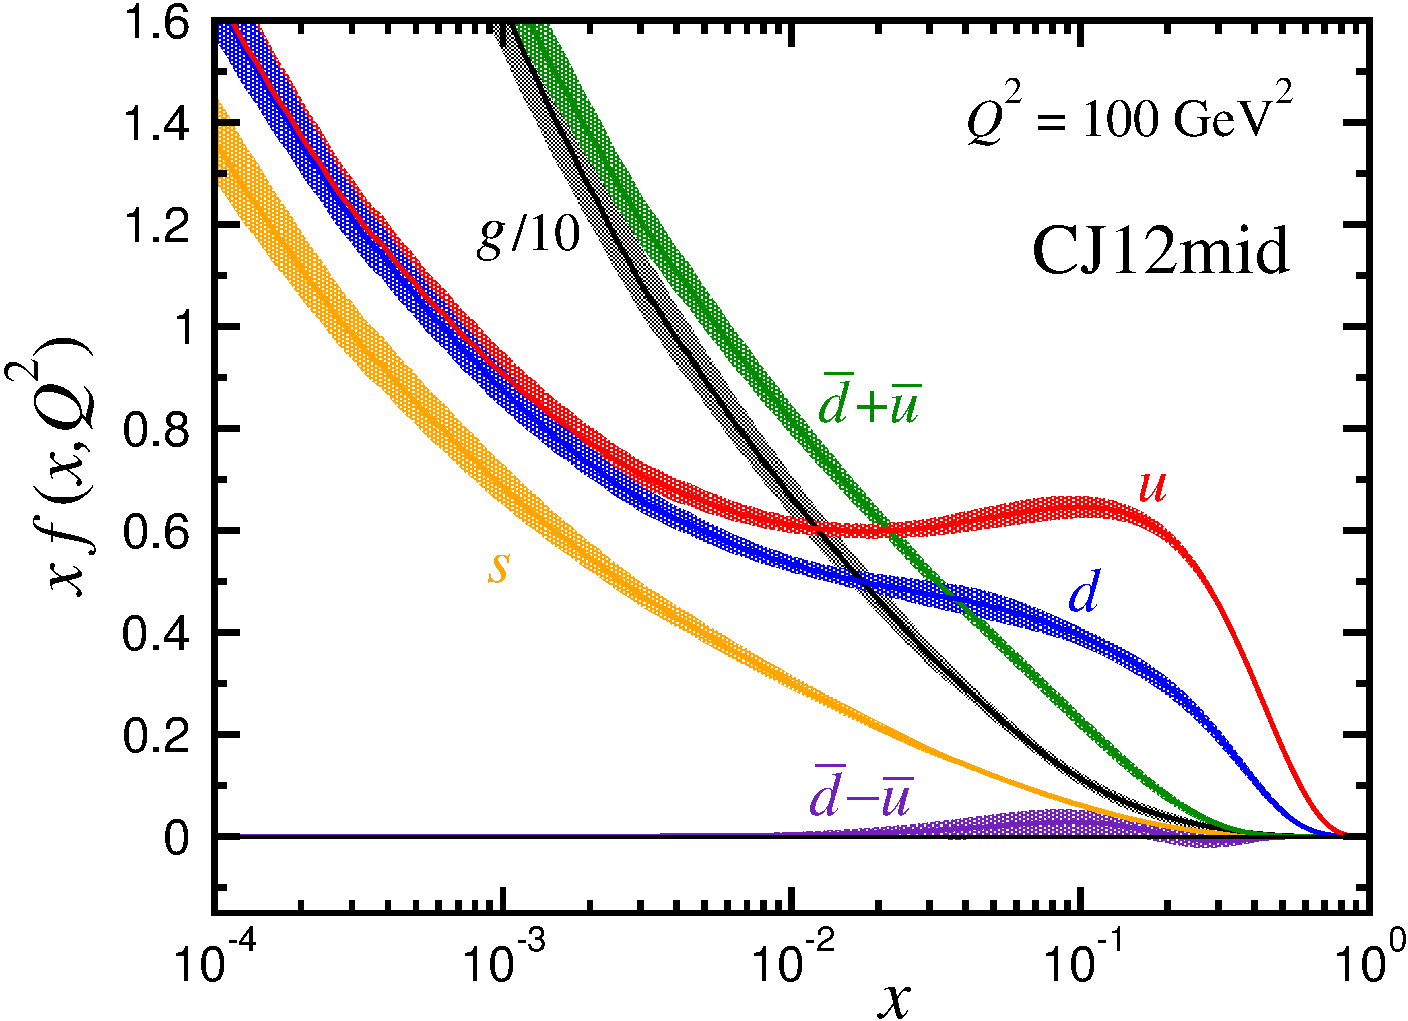
\includegraphics[width=0.6\textwidth]{chapitre3/figs/Fx_errl.pdf}
  \caption{PDFs pour divers partons issues du jeu de PDFs CJ12 \citep{Owens:2012bv}.}
  \label{fig:cj12}
\end{figure}


\subsection{L'hadronisation des partons : la gerbe partonique}

La majeure partie des particules produites lors de l'événement dur ne sont pas stables, et vont se désintégrer avant d'être détectées. Le cas des partons est encore plus complexe. Dans un premier temps, ils vont radier des gluons \emph{via} interaction forte, créant ainsi une gerbe partonique. Ensuite, étant des particules colorées, ils doivent obligatoirement se lier à d'autres partons afin de former des états non colorés (hadrons), c'est-à-dire neutre du point de vue de l'interaction forte. Ce processus est appelé hadronisation, et a lieu environ \SI{5e-24}{\s} après la production de la particule. Les hadrons ainsi formés peuvent ou non être stables. Lors de leur désintégration, les nouvelles particules produites vont à leur tour s'hadroniser. On obtient ainsi une cascade de désintégrations et d'hadronisations.

Ces effets sont très complexe à simuler, puisque à l'échelle d'énergie où ils se produisent, la QCD devient non-perturbative. Des programmes dédiés permettent néanmoins de simuler toute la chaîne d'hadronisation des particules, chacun utilisant des algorithmes spécialisés afin de simuler au mieux le développement de la gerbe partonique et de la chaine d'hadronisation. Parmi ces programmes, on peut citer \texttt{PYTHIA} \citep{pythia} et \texttt{HERWIG} \citep{Corcella:2000bw}.

\section{Simulation des événements}

Une fois l'hadronisation terminée, on dispose d'une liste de particules créées lors de la collision. Avant de pouvoir comparer les prédictions théoriques aux données collectées, il reste encore à simuler la réponse du détecteur. Deux approches sont possibles : une simulation détaillée, basée sur \texttt{GEANT 4} \citep{Agostinelli2003250}, mais très coûteuse en temps de calcul, et une moins détaillée, mais extrêmement plus rapide. Chaque méthode permet, grâce à des algorithmes différents, de simuler :
\begin{itemize}
    \item Le passage des particules dans le détecteur
    \item Les courbures des trajectoires des particules chargées par le champ magnétique
    \item Les gerbes électromagnétiques et hadroniques
    \item Les interactions particules - matières
    \item La réponse électrique des détecteurs
\end{itemize}

En plus de la liste ci-dessus, la simulation est aussi responsable de la désintégration des particules instables produites lors de la génération. En effet, la notion de stabilité dépend de l'échelle de temps considérée : une particule ne se désintégrant pas avant un temps $\tau$ est considérée comme stable. Ainsi, une particule peut être vue stable par le générateur Monte Carlo, mais instable par la simulation. Cette particule se désintègre donc à l'intérieur du détecteur, et cet effet doit être pris en compte pour une simulation complète.

\medskip

On décrit rapidement les deux méthodes de simulation ci-dessous.

\subsection{La simulation complète du détecteur}

Cette simulation repose sur une description extrêmement précise du détecteur. Ainsi, une réplique détaillée du détecteur est créée en 3 dimensions, comprenant même le câblage électrique des divers sous-détecteurs. Ce modèle est ensuite utilisé par le logiciel \texttt{GEANT 4}, qui va simuler la propagation, l'interaction, les diffusions multiples et la réponse des détecteurs pour chacune des particules créées lors de la collision. C'est une simulation très coûteuse en temps de calcul : la simulation d'un événement peut atteindre jusqu'à 2 minutes selon la complexité de l'état final.

\subsection{La simulation rapide du détecteur}

Une solution de simulation plus rapide existe au sein de la collaboration. Développée spécialement pour CMS \citep{1742-6596-219-3-032053}, cette simulation utilise une géométrie simplifiée du détecteur, et considère que les matériaux des sous-détecteurs ont une densité constante. La simulation des interactions au sein des divers sous-détecteurs est approximée en se basant sur les simulations complètes du détecteur. Tout en étant beaucoup plus rapide (environ \SI{200}{\ms} par événement), cette simulation permet de reproduire la plupart des observations avec une erreur de l'ordre du pourcent. Elle est très utilisée pour les études de mise-à-jour des détecteurs, où il est nécessaire de pouvoir simuler très rapidement l'effet d'une modification du détecteur sur les observables physiques.

\section{Reconstruction des événements}

La reconstruction d'un événement est effectuée de façon identique, que ça soit de la simulation ou une prise de données réelle. En effet, la simulation du détecteur fournit en sortie les signaux électriques des sous-détecteurs, de façon identique à ce qui se passe lors des vraies collisions.

\subsection{L'algorithme \emph{Particle-Flow} (PF)}

CMS utilise un algorithme spécialisé pour reconstruire les objets physiques : l'algorithme du \emph{particle-flow} \citep{pf,cms_pf_2,cms_pf_jets,cms_pf_leptons}. En utilisant l'information de tous les sous-détecteurs pour reconstruire l'événement, cet algorithme permet d'améliorer significativement la résolution des particules reconstruites, et s'avère être un moyen efficace de contrebalancer les faiblesses de HCAL : on peut en effet utiliser l'excellente performance du trajectographe pour aider à la reconstruction des hadrons chargés.

Le \emph{particle-flow} permet de reconstruire les 5 types de particules stables détectées par CMS : les électrons, les muons, les photons, et certains hadrons neutres et chargés. Ces particules sont ensuite utilisées comme des briques élémentaires pour reconstruire des objets plus complexes, comme les jets. Ces briques étant ensuite utilisées par les analyses de physique, il est primordial que le \emph{particle-flow} possède une efficacité de reconstruction la plus haute possible, tout en ayant un taux de fausse identification le plus faible possible. Ces contraintes ont conduit à l'élaboration d'algorithmes dédiés de trajectographie et de calorimétrie, détaillés ci-dessous.

\subsubsection{Trajectographie itérative} \label{sec:tracks_reconstruction}

L'impulsion des hadrons est mesurée avec une résolution bien meilleure par le trajectographe que par les calorimètres. Comme près de \sfrac{2}{3} de l'énergie d'un jet est due à la présence de hadrons chargés, le trajectographe joue un rôle majeur dans la performance du \emph{particle-flow}.

Afin de reconstruire les trajectoires des particules avec une grande efficacité, tout en conservant un taux de faux minimal, une procédure itérative \citep{cms_tracks}, basée sur un filtre de Kalman (KF), est employée. La reconstruction commence en utilisant seulement les \emph{hits} des deux premières couches du détecteur à pixels, ainsi que la position du vertex primaire. C'est ce qu'on appelle la graine de l'algorithme. On cherche ensuite à compléter la trajectoire en utilisant les \emph{hits} des autres couches du trajectographe. Les contraintes lors de cette première étape sont vraiment fortes, ce qui conduit à une efficacité de reconstruction moyenne, mais à un très faible taux de faux.

Avant l'étape suivante, les \emph{hits} associés de façon certaine à une trajectoire sont enlevés de la liste des \emph{hits} disponibles, et on réitère ensuite la même procédure en relâchant un peu les contraintes, ce qui permet d'améliorer l'efficacité de reconstruction, tout en gardant un taux de faux très faible grâce à la réduction du nombre de combinaison. Après la troisième itération, on obtient une efficacité de reconstruction de \SI{99.5}{\%} pour les muons isolés et de plus de \SI{90}{\%} pour les hadrons chargés. Pour les quatrième et cinquième itérations, la contrainte sur le point d'interaction est relâchée, ce qui permet de reconstruire les trajectoires des hadrons chargés secondaires ayant un vertex d'interaction déplacé.

Grâce à cet algorithme de trajectographie itérative, la trajectoire d'une particule chargée ne laissant que 3 \emph{hits}, avec un $p_T$ de seulement \SI{150}{\MeV} et un vertex de production éloigné de plus de \SI{50}{\cm} de l'axe du faisceau est reconstruite avec un taux de faux de l'ordre du pourcent. On peut voir figure \ref{fig:iterative_tracking_eff} l'efficacité de reconstruction des trajectoires grâce à l'utilisation de l'algorithme de trajectographie itératif.

\begin{figure} \centering
  \subcaptionbox{\label{fig:tracking_eff_mu}}[0.45\textwidth]{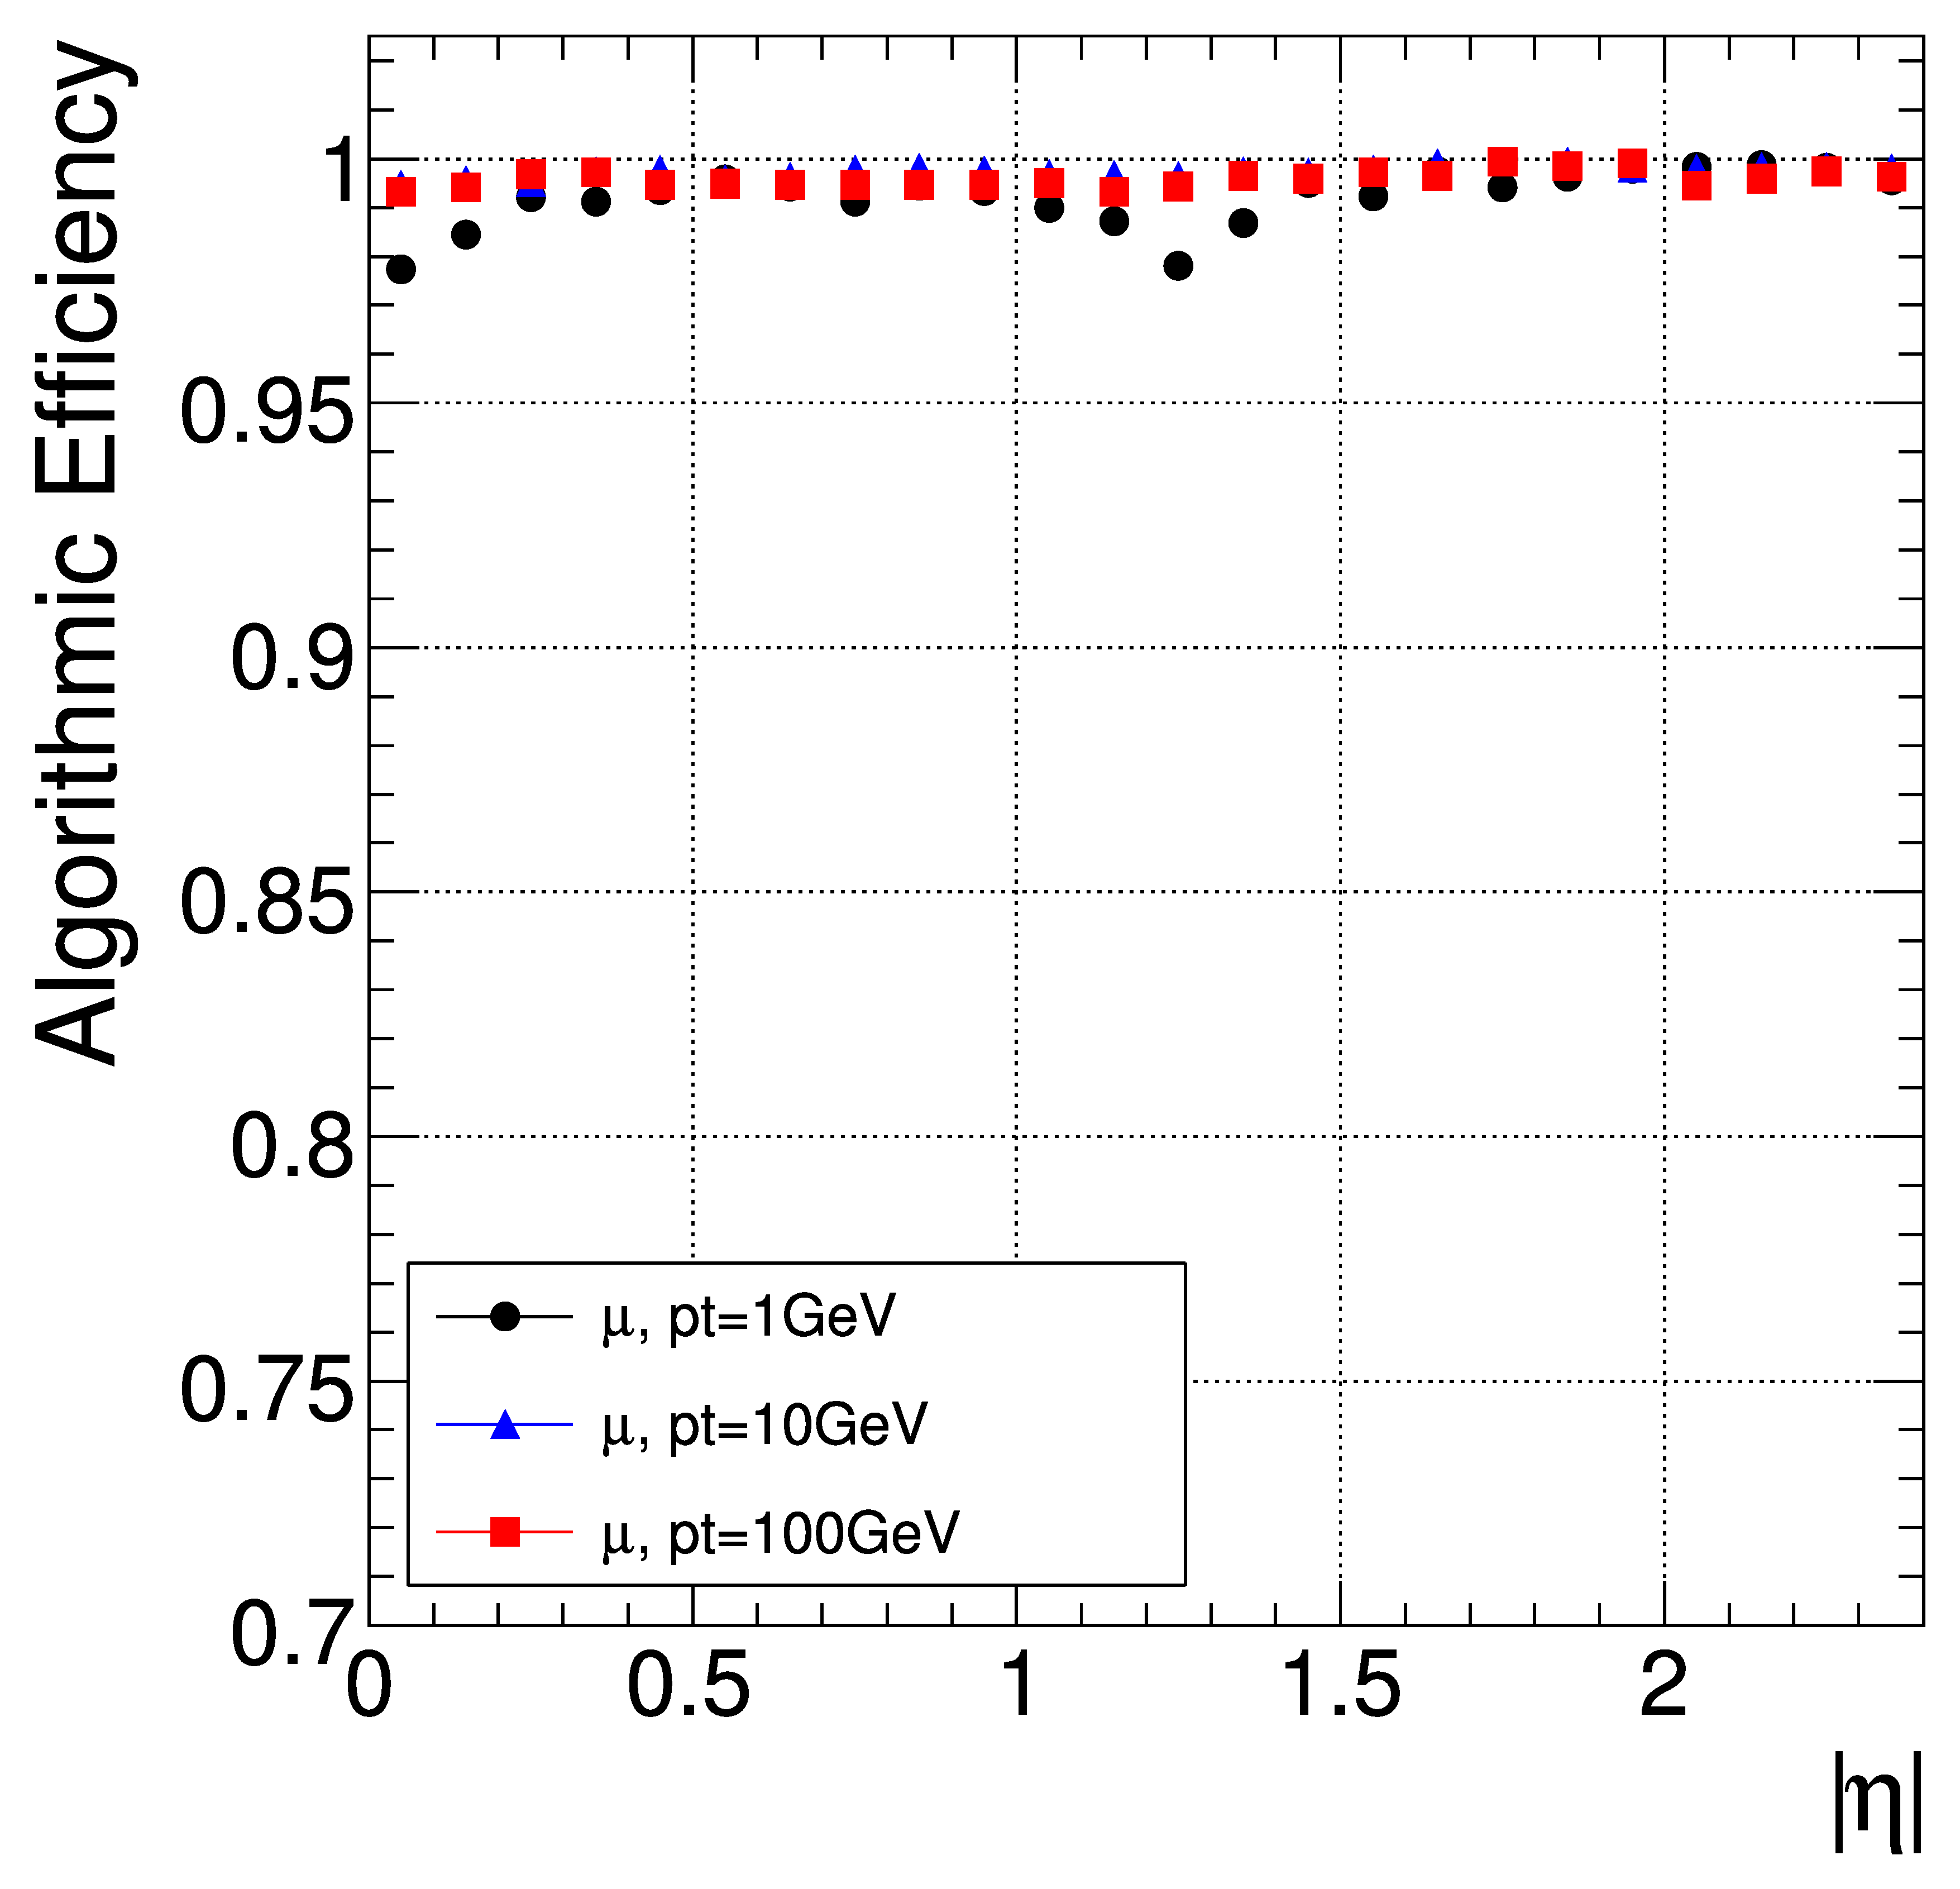
\includegraphics[width=0.45\textwidth]{chapitre3/figs/iterative_tracking_mu.pdf}}\hfill
  \subcaptionbox{\label{fig:tracking_eff_pi}}[0.45\textwidth]{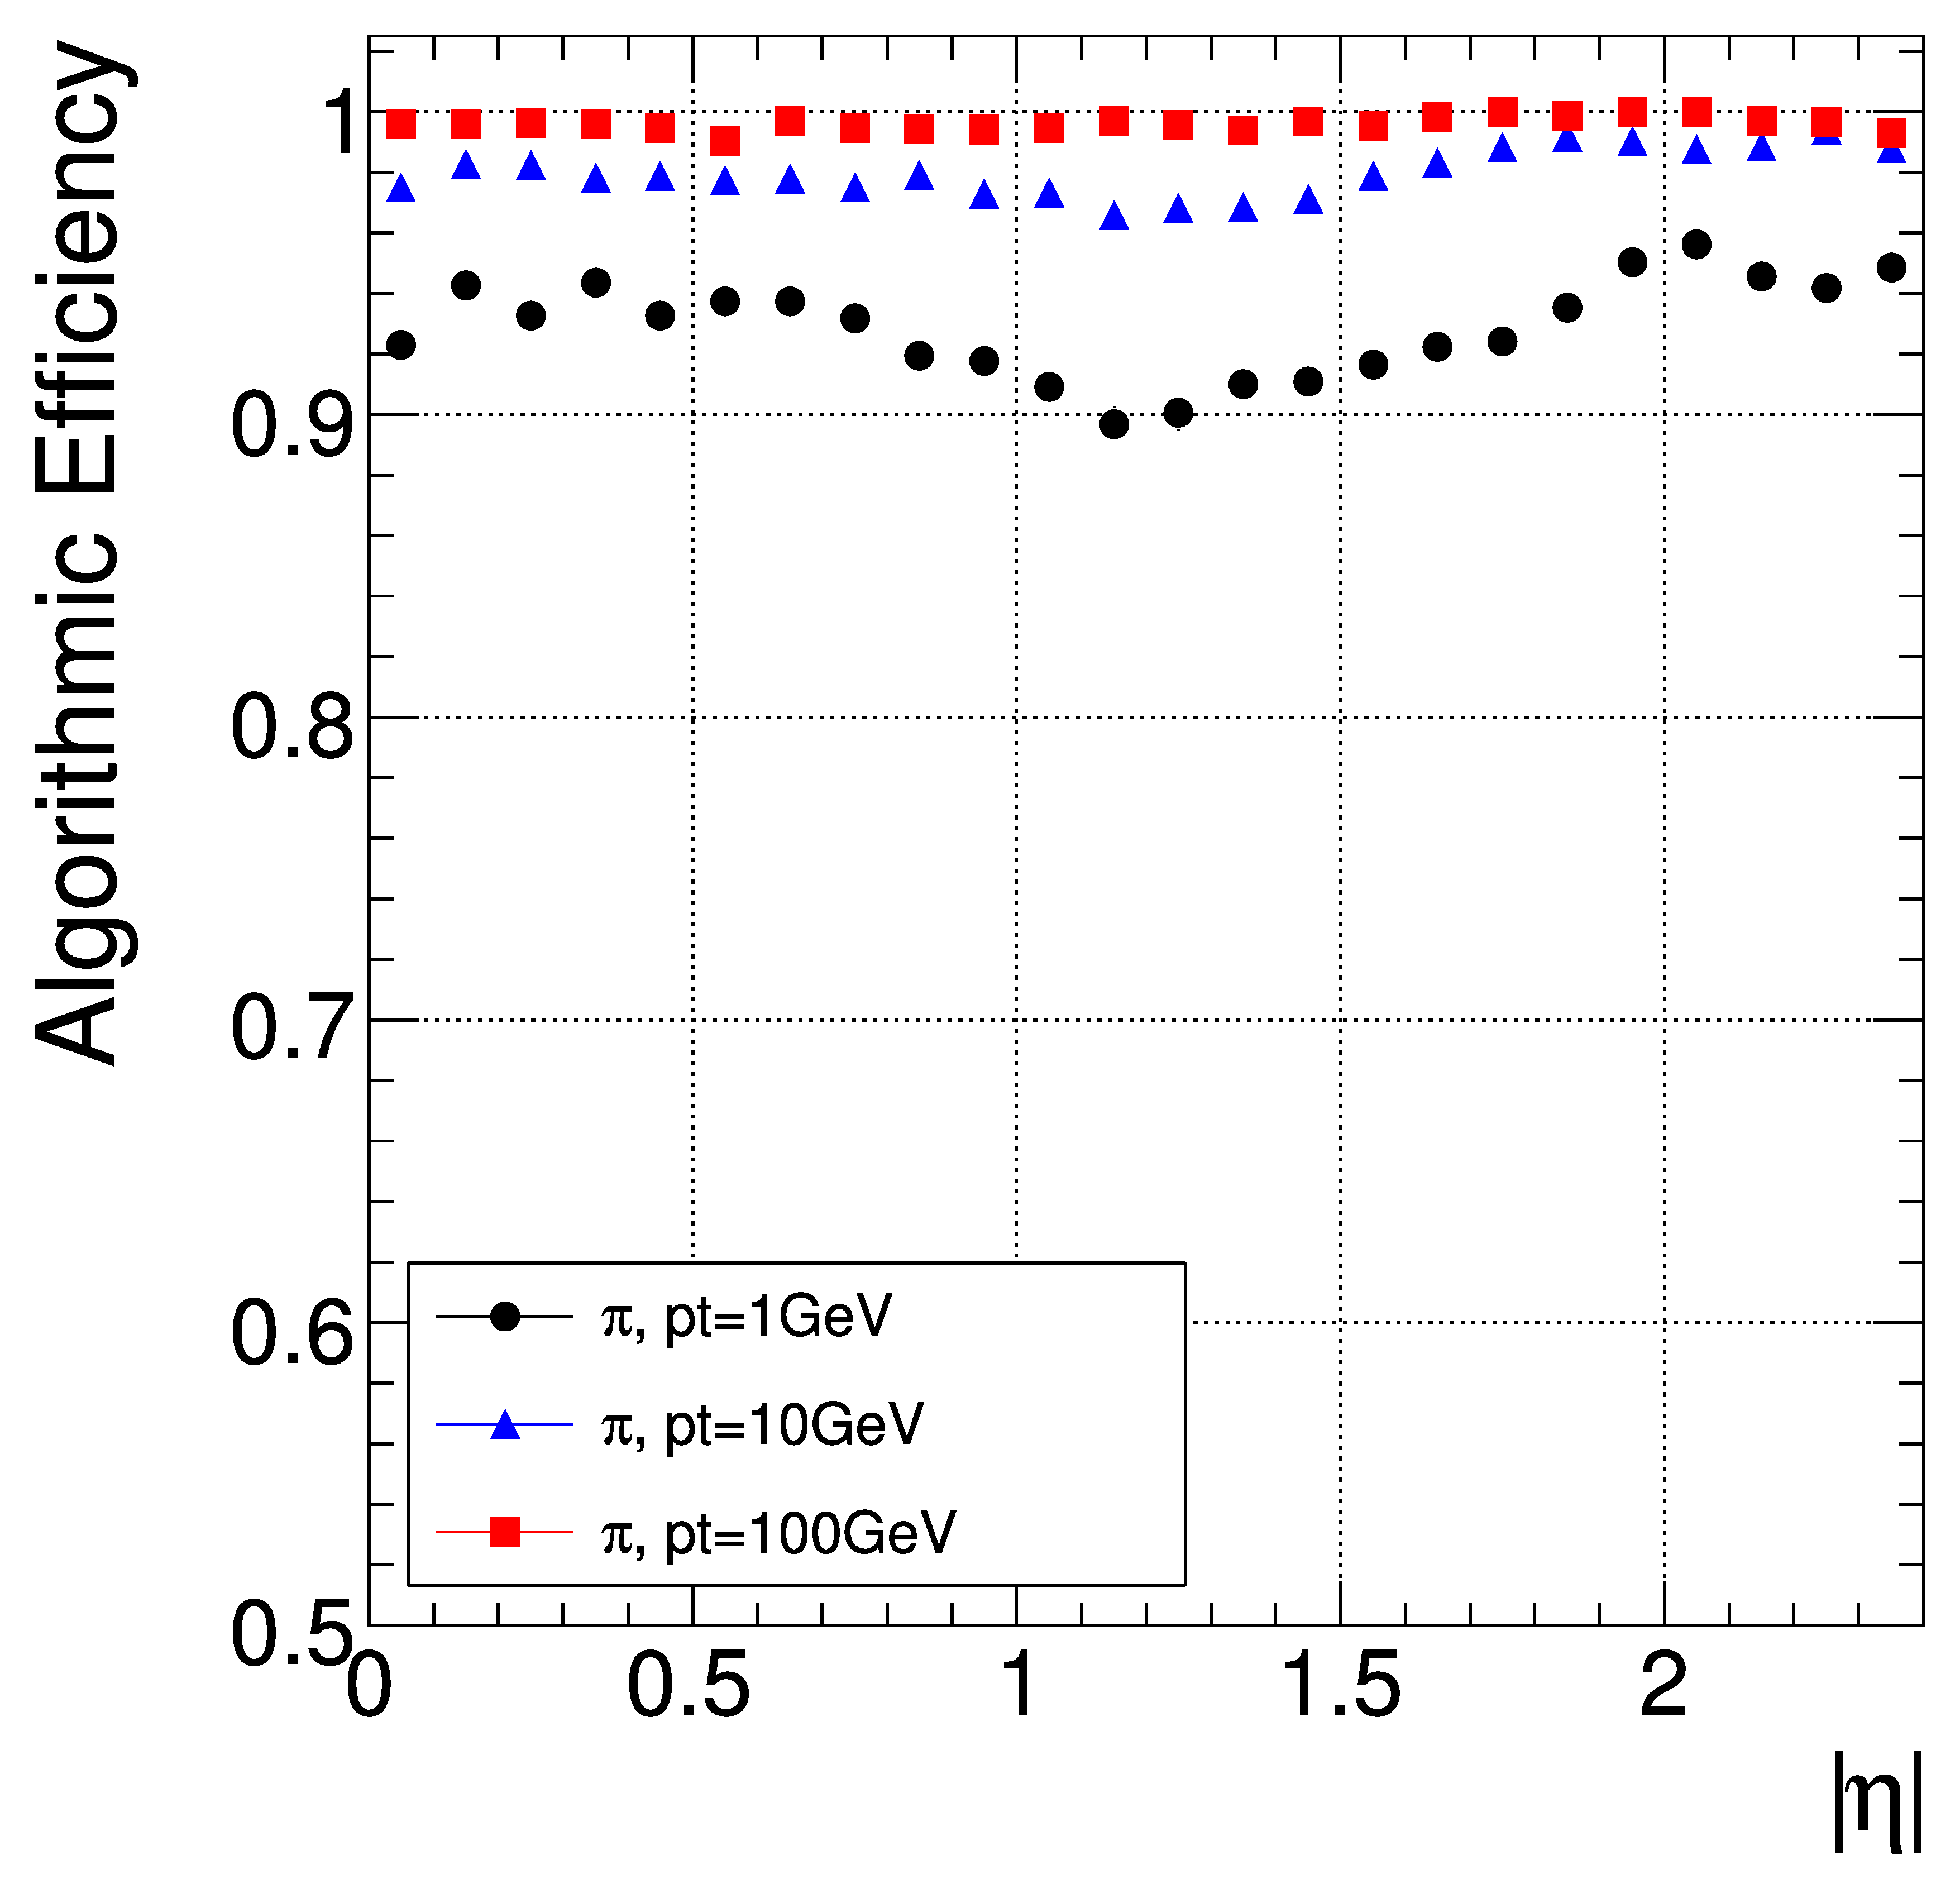
\includegraphics[width=0.45\textwidth]{chapitre3/figs/iterative_tracking_pi.pdf}}
  \caption{Efficacité de reconstruction des trajectoires pour des muons (\subref{fig:tracking_eff_mu}) et pour des pions (\subref{fig:tracking_eff_pi}).}
  \label{fig:iterative_tracking_eff}
\end{figure}

\subsubsection{Agglomération calorimétrique}

Un algorithme d'agglomération calorimétrique cherche à atteindre 4 buts :
\begin{enumerate}
  \item Mesurer l'énergie et la direction des particules neutres (photons, hadrons neutres).
  \item Séparer les dépôts d'énergies des particules neutres de ceux des particules chargées.
  \item Reconstruire les électrons et le rayonnement Bremsstrahlung associé.
  \item Aider à la mesure de l'énergie des hadrons chargés pour lesquels la trajectoire n'a pas été bien reconstruite (hadrons de bas \pt).
\end{enumerate}

L'algorithme spécifique développé pour le \emph{particle-flow} permet d'atteindre une très haute efficacité de reconstruction, tout en gardant un grand pouvoir de séparation des dépôts d'énergie. L'agglomération est effectuée de façon séparée dans chaque sous-calorimètre (tonneau du ECAL, tonneau du HCAL, bouchons du ECAL et HCAL, \ldots), et ce en trois phases.

\medskip

\begin{figure}
  \subcaptionbox{\label{fig:calo_topo}}[0.45\textwidth]{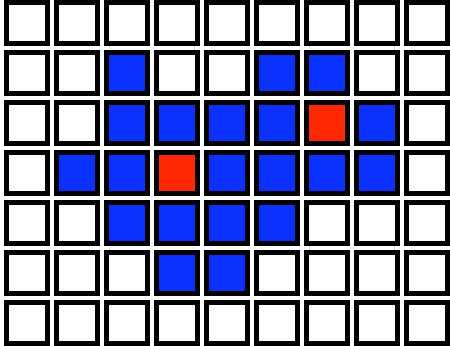
\includegraphics[width=0.45\textwidth]{chapitre3/figs/calo_topoclus_seeds.pdf}}\hfill
  \subcaptionbox{\label{fig:calo_depth}}[0.45\textwidth]{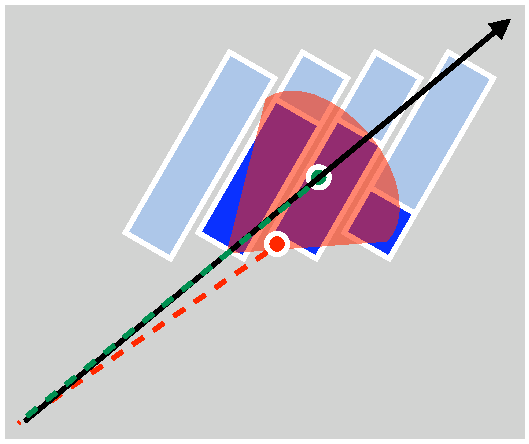
\includegraphics[width=0.45\textwidth]{chapitre3/figs/calo_depthcor.pdf}}
  \caption{Agglomérat topologique contenant deux graines (\subref{fig:calo_topo}) et détermination de la profondeur du dépôt d'énergie (\subref{fig:calo_depth}). En rouge, la position déterminée sans tenir compte de la profondeur biaise \aeta. En vert, la profondeur est correctement estimée.}
\end{figure}

Premièrement, on identifie les graines de l'algorithme comme les cellules calorimétriques où l'énergie dépasse un certain seuil, fixé à une valeur supérieure au niveau de bruit du détecteur. Les cellules en contact avec une graine (4 ou 8 suivant la configuration) ne peuvent pas devenir des graines à leur tour. On construit ensuite des "agglomérats topologiques", en partant des graines et en agrégeant les cellules avec au moins un côté en commun avec la graine et avec une énergie au dessus d'un seuil, fixé comme deux fois la déviation standard du bruit électronique dans le ECAL (\SI{80}{\MeV} dans le tonneau, \tilde \SI{300}{\MeV} dans les bouchons) et à \SI{800}{\MeV} dans le HCAL. Il peut y avoir plusieurs graines dans un même agglomérat topologique. Dans ce cas, le partage de l'énergie entre chaque graine est effectuée selon la distance entre la cellule et la graine, en considérant que les gerbes électromagnétiques déposent leur énergie selon un profil gaussien, dont la largeur ne dépend pas de l'énergie.

\medskip

La position de l'agrégat est déterminée à partir de la graine et des 4 ou 8 cellules voisines, à l'aide de la formule
\begin{align*}
  X &= \frac{ \sum_i{w_i X_i} }{ \sum_i{w_i} }\text{, avec } w_i = \ln{\frac{E_i}{E_{th}}}
\end{align*}
avec $X = x, y$ ou $z$, $X_i$ la position de la cellule $i$, $E_i$ l'énergie de la cellule $i$, et $E_{th}$ le seuil d'énergie. Dans le cas où l'agrégat ne compte qu'une seule graine, toutes les cellules de l'agrégat sont utilisées pour calculer la position. Afin de ne pas introduire de biais en $\eta$ lors de la détermination de la position, on estime la profondeur du maximum de la gerbe électronique par la formule
\begin{align*}
  p &= a\left( b + \ln{E} \right)
\end{align*}
où $p$ est la profondeur, $a$ et $b$ sont des constantes qui dépendent de $\eta$, et $E$ l'énergie totale de l'agrégat. On peut voir figure \ref{fig:calo_depth} l'effet de cette procédure sur la détermination de la position angulaire de l'agrégat.

\subsubsection{L'algorithme de liaison} \label{sec:pf_links}

Il reste maintenant à lier ensemble les traces et les agrégats reconstruits puisqu'une particule peut déposer de l'énergie dans les divers sous-détecteurs, tout en éliminant toute possibilité de double comptage de l'énergie. L'algorithme produit donc des "blocs" d'éléments qui vont ensuite servir pour reconstruire les particules. Grâce à l'excellente granularité de CMS, chaque bloc compte en moyenne 2-3 éléments, ce qui permet aux algorithmes de reconstruction des particules de rester extrêmement performants, et ce même quand les événements deviennent très complexes.

\paragraph{Les liens traces – agrégats calorimétriques}

Les traces reconstruites dans le trajectographe sont extrapolées :
\begin{itemize}
  \item Dans le calorimètre électromagnétique, jusqu'à une profondeur correspondant au maximum attendu d'une gerbe électromagnétique.
  \item Dans le calorimètre hadronique, jusqu'à une profondeur d'une interaction nucléaire ($\lambda_0$, voir \cref{sec:hcal}), longueur caractéristique d'une gerbe hadronique.
\end{itemize}

On relie la trace à un agrégat si la position extrapolée de la trace passe dans la zone délimitée par l'agrégat. Cette zone peut être augmentée d'une unité (un cristal pour le ECAL, ou une tour pour le HCAL) dans chaque direction, afin de tenir compte de possibles trous entre les modules calorimétriques, de l'incertitude sur la profondeur du maximum de la gerbe, et enfin des multiples diffusions des particules de très bas \pt. On peut voir figure \ref{fig:pf_links} la connexion entre deux traces et des agrégats calorimétriques pour un événement enregistré en décembre 2009 par CMS. On définit la distance du lien par la distance $\Delta R = \sqrt{\eta^2 + \phi^2}$ dans le plan ($\eta$, $\phi$).

\begin{figure}
  \subcaptionbox{ECAL\label{fig:pf_links_ecal}}[0.45\textwidth]{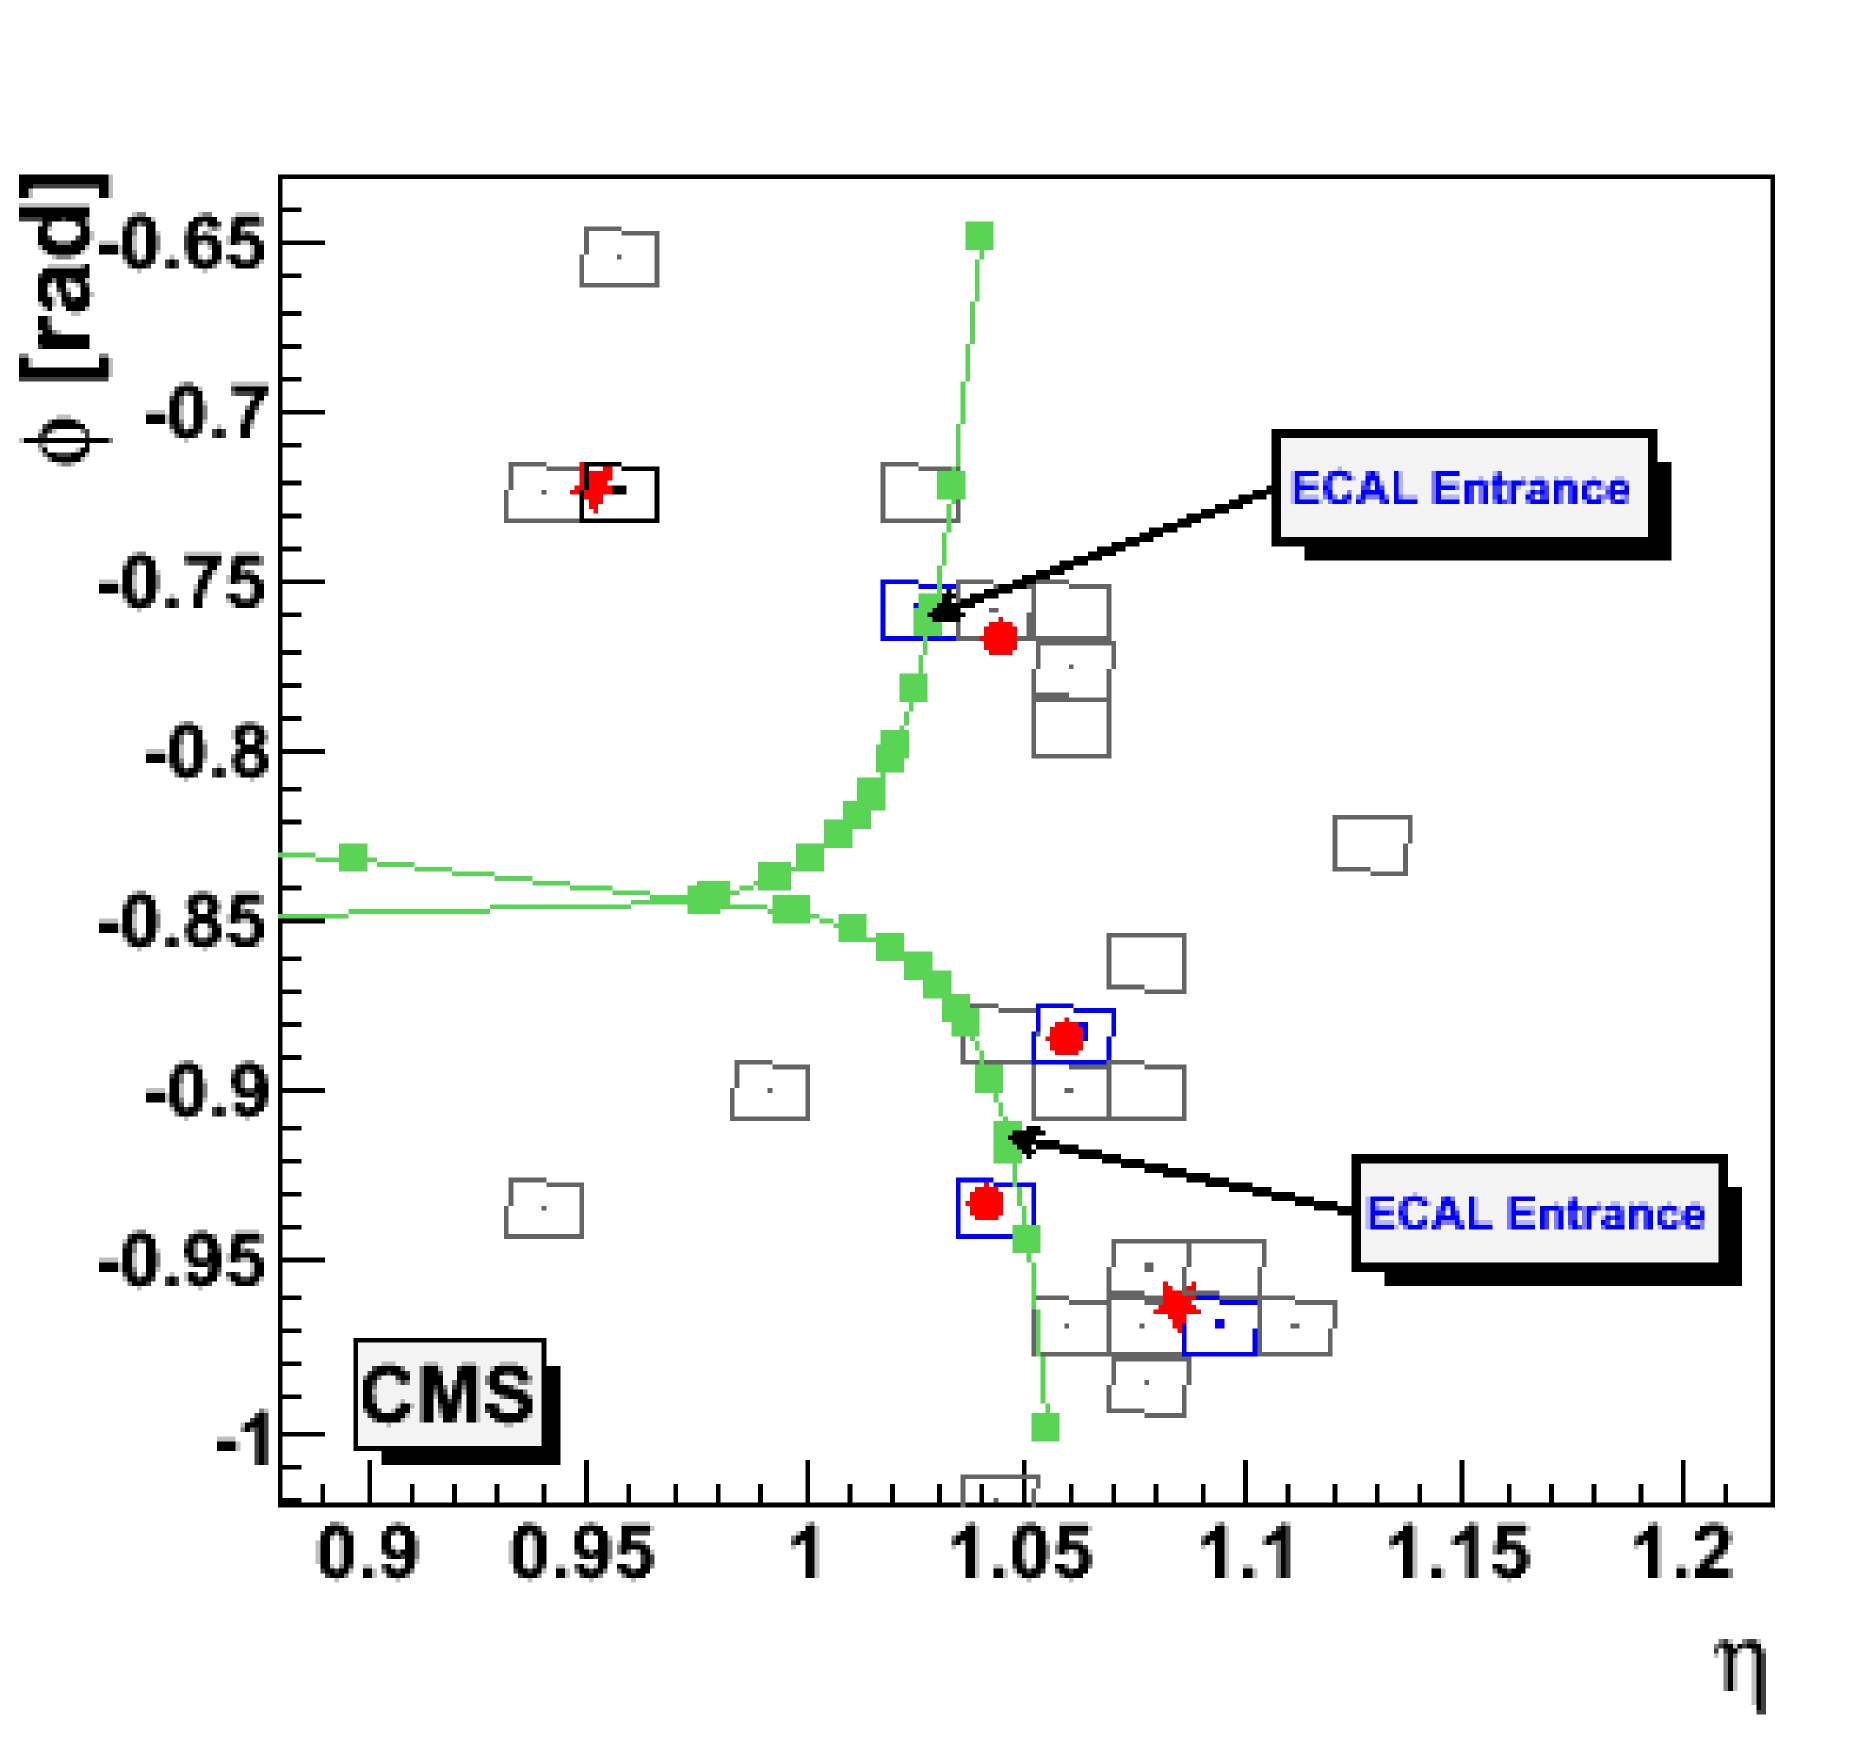
\includegraphics[width=0.45\textwidth]{chapitre3/figs/pf_links_ecal.png}}\hfill
  \subcaptionbox{HCAL\label{fig:pf_links_hcal}}[0.45\textwidth]{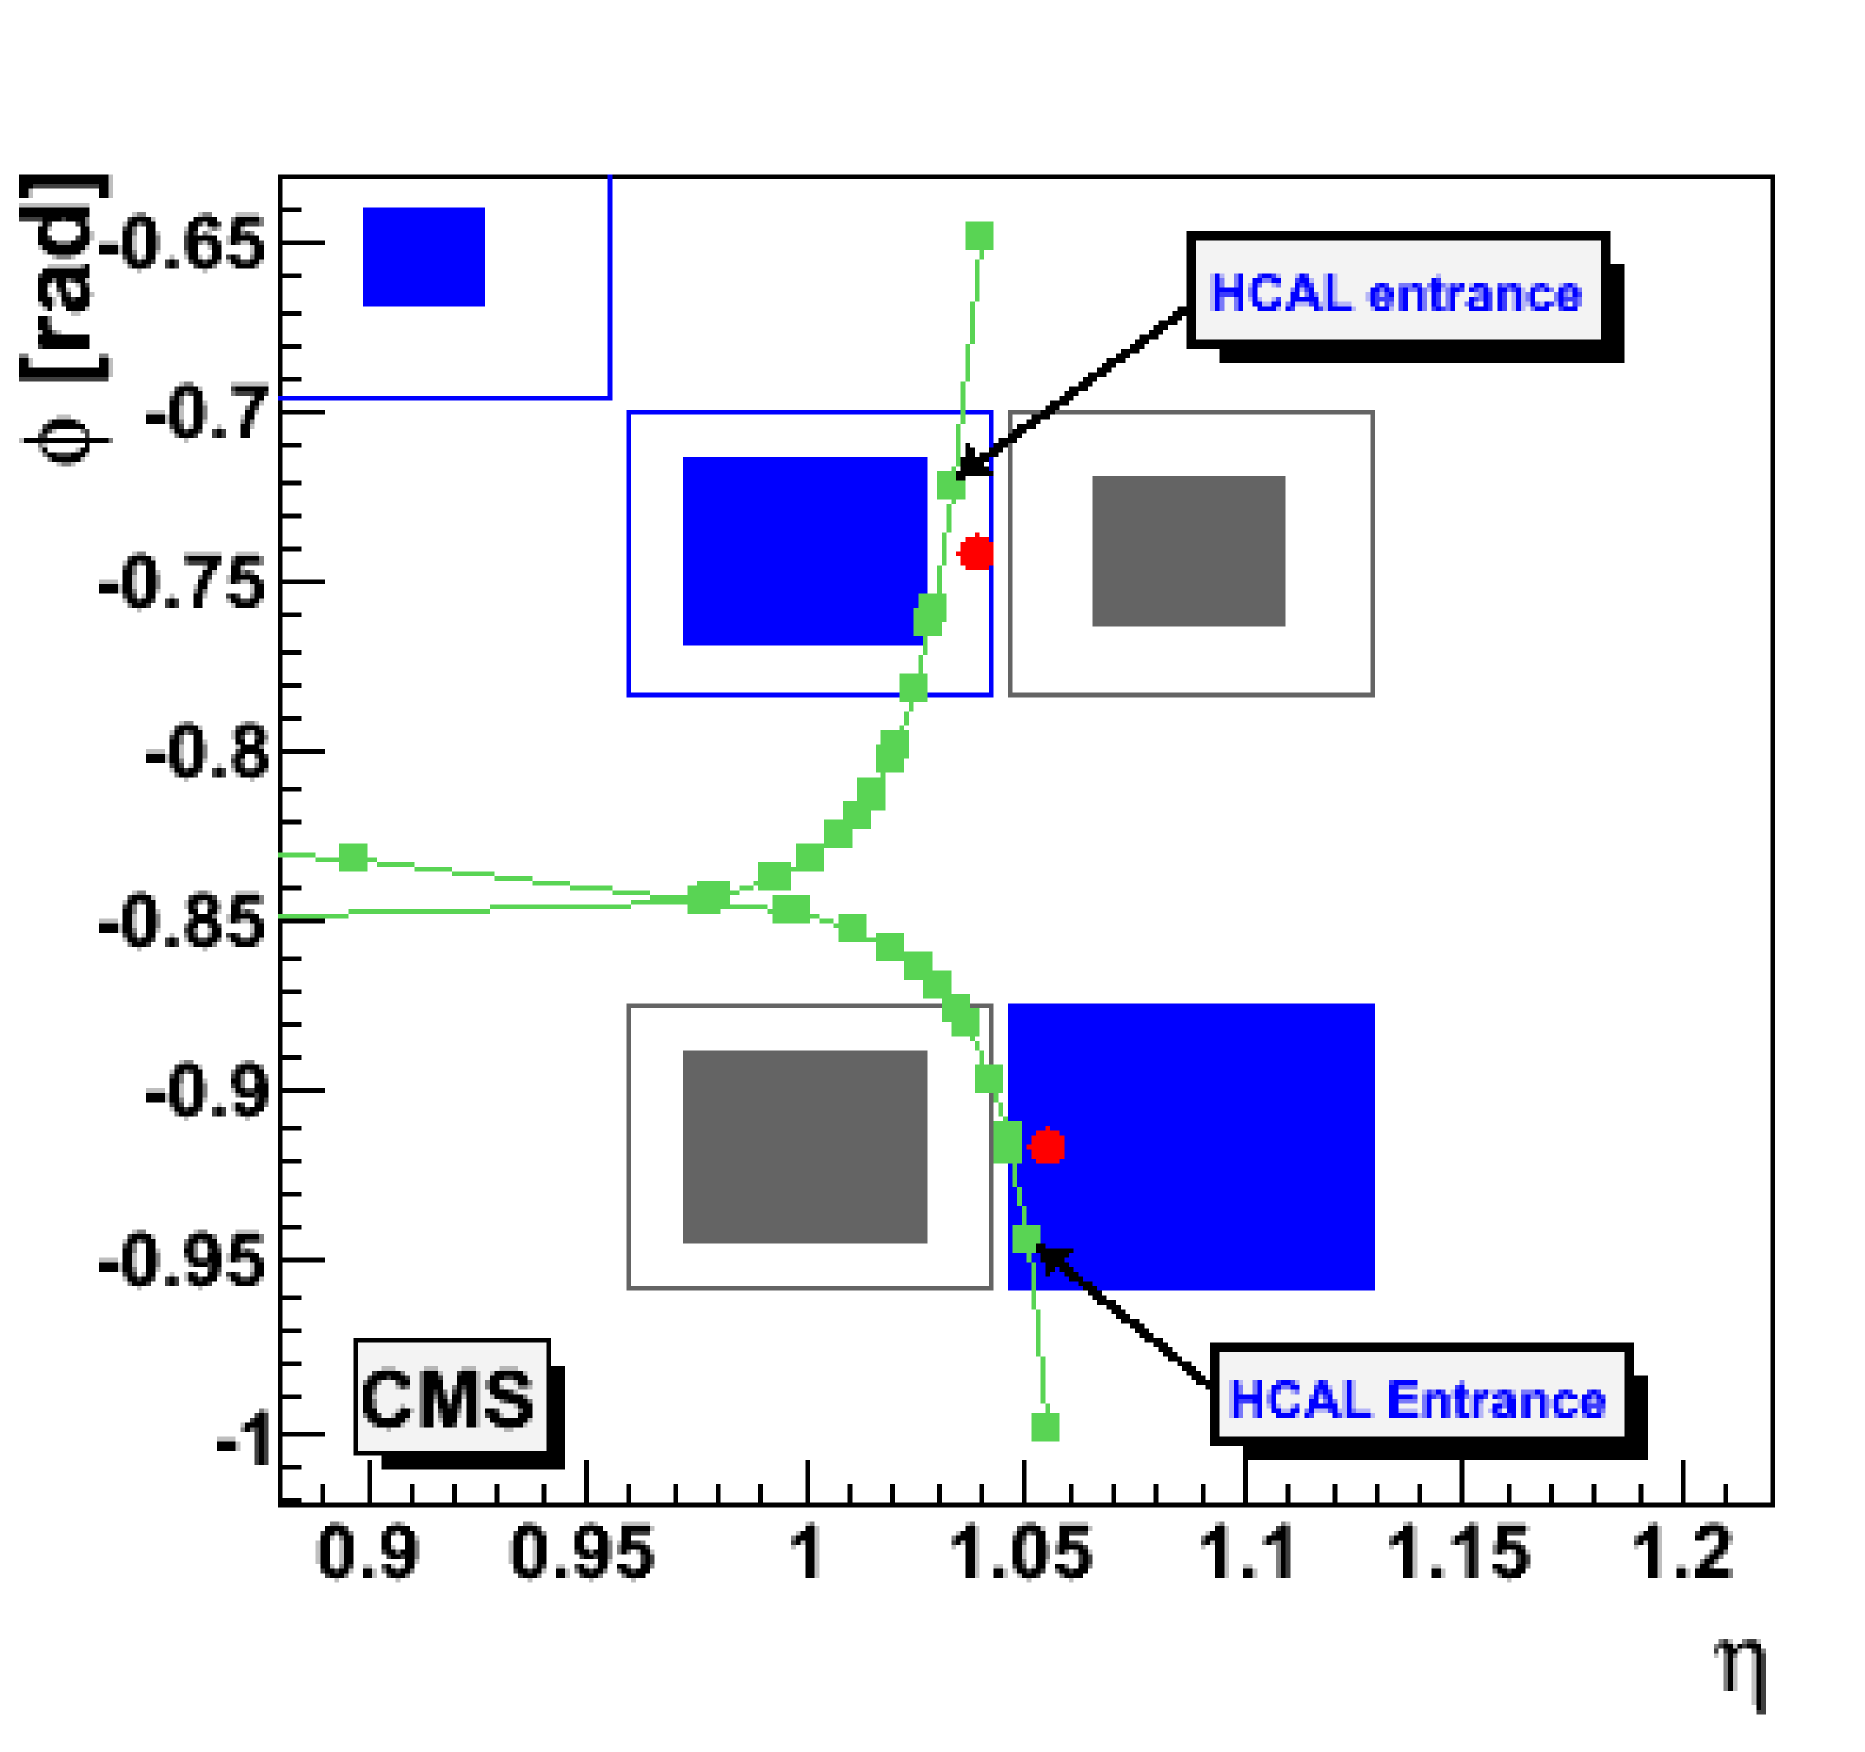
\includegraphics[width=0.45\textwidth]{chapitre3/figs/pf_links_hcal.png}}
  \caption{Connexion entre les traces et les agrégats calorimétriques. Les traces (les lignes vertes avec marqueurs carrés) sont liées avec un ou deux agrégats dans le ECAL (\subref{fig:pf_links_ecal}) et un agrégat dans le HCAL (\subref{fig:pf_links_hcal}). Chaque carré gris représente une cellule calorimétrique. Les ronds rouges représentent les agrégats liés à une trace, alors que les étoiles rouges sont les agrégats non liés.}
  \label{fig:pf_links}
\end{figure}

Afin de collecter l'énergie perdue par les électrons par rayonnement Bremsstrahlung, des trajectoires tangentes à la trajectoire principale sont extrapolées dans le ECAL. Un agrégat est lié à la trace principale comme candidat photon Bremsstrahlung si la trajectoire extrapolée passe dans la zone de l'agrégat, comme défini juste avant.

\paragraph{Les liens ECAL – HCAL}

De façon similaire, un lien entre les deux calorimètres est créé lorsque la position de l'agrégat formé dans le calorimètre électromagnétique est contenu dans la zone limitée par l'agrégat formé dans le calorimètre hadronique. L'enveloppe des agrégats peut ici aussi être agrandie d'une unité de chaque côté. La distance du lien est donné par $\Delta R$. %dans le plan ($\eta$, $\phi$).

\paragraph{Les liens trajectographe – détecteur à muons} \label{sec:pf_link_mu}

Le spectromètre à muons reconstruit aussi des traces. Un lien est fait (qu'on appelle muon global) avec les traces du trajectographe lorsque l'ajustement entre les deux traces donne un $\chi^2$ acceptable. Si une trace dans le détecteur à muons peut être associée à plusieurs traces dans le trajectographe, le lien est fait entre les deux traces qui donnent le plus petit $\chi^2$. Pour ce type de lien, la distance du lien est donnée par le $\chi^2$.

\subsection{L'identification des particules}

Après application de l'algorithme de liaison (voir \cref{sec:pf_links}), on dispose d'une liste de blocs, composés chacun d'environ 2-3 éléments (traces ou agrégats calorimétriques). Il reste maintenant à identifier chaque bloc en tant que particule. Cette identification conduira à la création d'une liste de particules, donnant une description globale de l'événement.

\subsubsection{Reconstruction des muons} \label{sec:muon_reco}

Les premières particules à être reconstruites sont les muons \citep{cms_muons_reco}, avant même le début de la reconstruction de l'événement grâce au \emph{particle-flow}. Les muons laissant des traces à la fois dans le trajectographe et dans le spectromètre à muons, deux types de reconstructions sont utilisées :

\begin{description}
    \item[Reconstruction des muons globaux] Pour chaque trace dans le spectromètre à muons, on cherche par extrapolation une trace correspondante dans le trajectographe, afin de déterminer une trace globale grâce à une interpolation des deux trajectoires. Cette technique est similaire à celle utilisée dans l'algorithme de lien trajectoire -- détecteur à muons présenté \cref{sec:pf_link_mu}. A haute impulsion transverse ($\pt \gtrsim \SI{200}{\GeV}$), cette méthode permet d'améliorer la résolution de l'impulsion comparée à l'utilisation de la trace du trajectographe uniquement.
    \item[Reconstruction des \emph{tracker} muons] On ne considère ici que les traces présentes dans le trajectographe comme possibles candidats muons. Ces traces sont extrapolées jusqu'au détecteur à muons, en prenant en compte les pertes d'énergie et l'incertitude due aux multiples diffusions. Si au moins un segment\footnote{Un segment correspond à une petite trace dans le spectromètre à muons, composée de quelques \emph{hits} de DT ou CSC.} dans le spectromètre coïncide avec la trajectoire extrapolée, la trace est identifiée comme un muon. Pour les muons de faible impulsion ($\pt \lesssim
 \SI{5}{\GeV}$), cette approche est plus performante que la reconstruction des muons globaux, puisqu'il est nécessaire d'avoir un seul segment qui coïncide, au lieu de plusieurs pour l'autre méthode.
\end{description}

La majorité des muons sont reconstruits comme muons globaux ou \emph{tracker} muons, voire comme les deux. Cependant, pour environ \SI{1}{\%} des muons, aucune trace n'est trouvée dans le trajectographe. On classe donc ces muons dans une troisième catégorie, les muons \emph{standalone}.

\medskip

\begin{figure}[tbp]
    \centering
    \subcaptionbox{\label{fig:dimu_jpsi}}[0.49\textwidth]{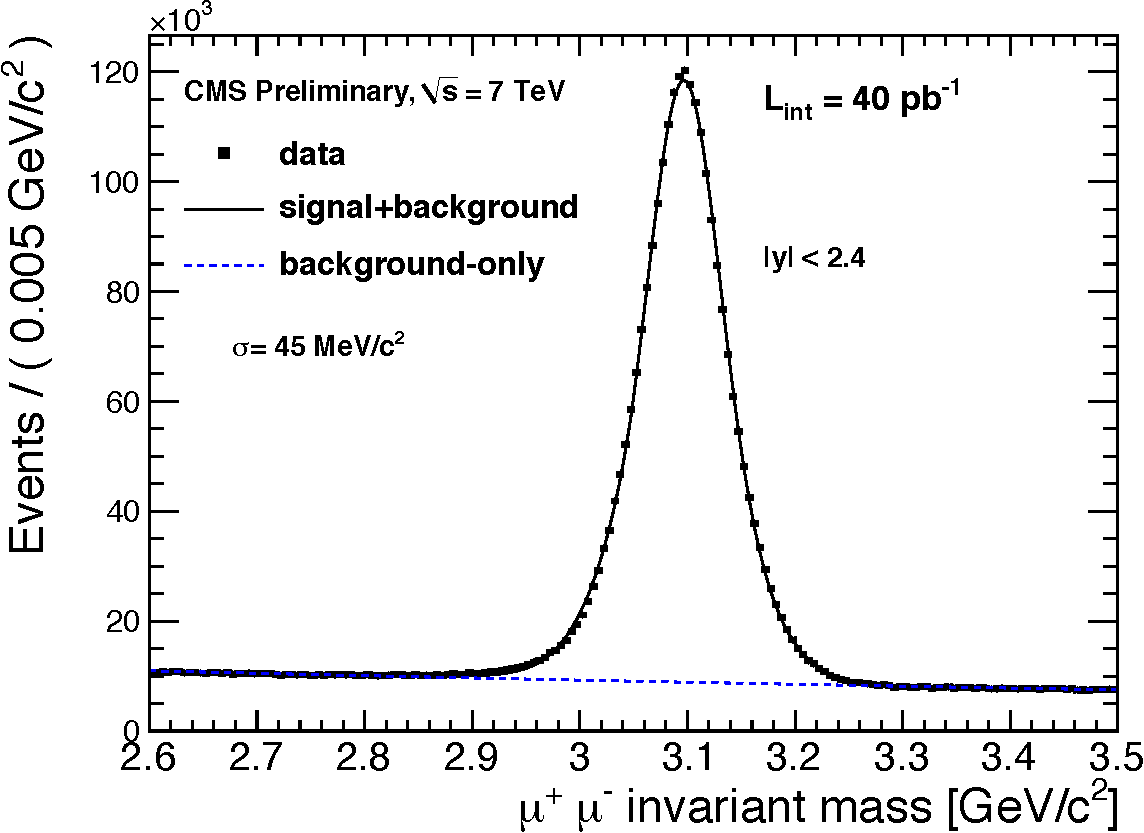
\includegraphics[width=0.49\textwidth]{chapitre3/figs/JPsi40pb-1.pdf}} \hfill
    \subcaptionbox{\label{fig:dimu_mass}}[0.49\textwidth]{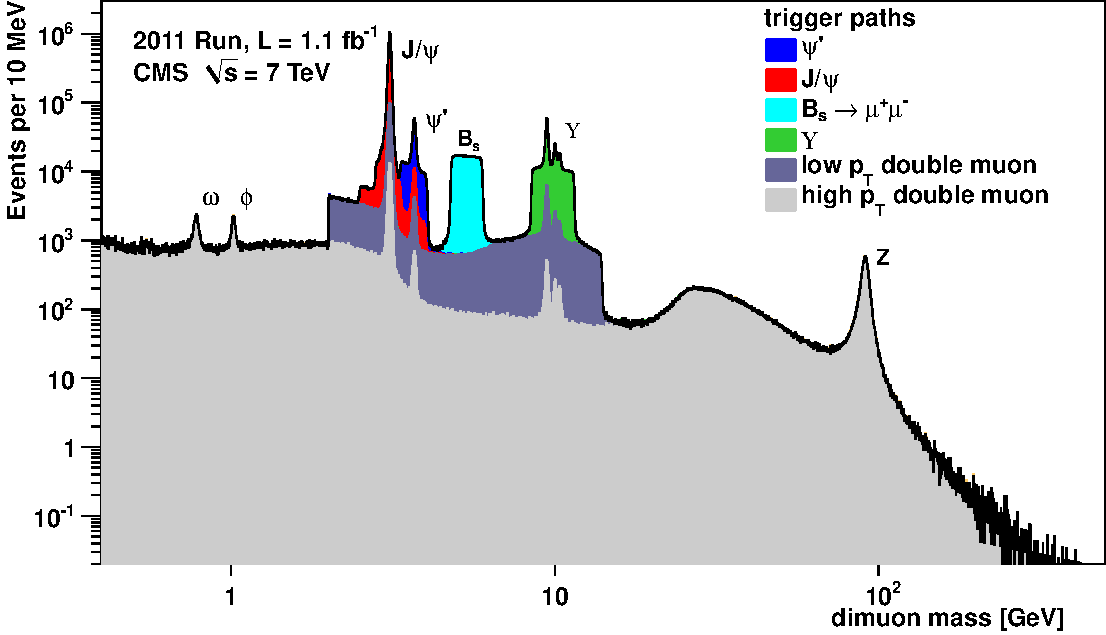
\includegraphics[width=0.49\textwidth]{chapitre3/figs/mass_dimu.pdf}}
    \caption{(\subref{fig:dimu_jpsi}) Comparaison entre la simulation et les données pour des événements $\PJpsi \rightarrow \Pmuon \APmuon$, reconstruit à l'aide des données 2010. La résolution sur la reconstruction du pic de masse du \PJpsi est de $\SI{45}{\MeV}$. (\subref{fig:dimu_mass}) Spectre de masse invariante di-muons reconstruit à l'aide des données 2011. L'excellente résolution permet même de reconstruire les résonances $\omega$ et $\phi$.}
    \label{fig:dimu_mass_spectrum}
\end{figure}

On regroupe ensuite les trois catégories de muons dans une liste de candidats muons. Les candidats muons globaux et \emph{tracker} muons qui partagent la même trace du trajectographe sont fusionnés en un seul candidat.

Afin d'identifier les muons \emph{particle-flow}, une sélection est effectuée sur les candidats muons reconstruits avec l'algorithme standard. On dénombre trois sélections différentes : "isolé", "\emph{pf-tight}" et "\emph{pf-loose}". Les muons sont considérés isolés si, dans un cône de taille $R = \num{0.3}$ centré sur le muon, la somme du \pt des traces et des agrégats calorimétriques est inférieure à \SI{10}{\%} de l'impulsion du muon. Dans ce cas, l'effet du \emph{particle-flow} est limité puisque l'environnement immédiat autour du muon est propre. Par conséquent, une grande efficacité est obtenue en appliquant une sélection peu contraignante : les muons doivent seulement être des muons globaux.

Une fois les muons isolés traités, les sélections \emph{pf-loose} et \emph{pf-tight} sont appliquées aux muons restants. Ces deux sélections sont optimisées pour identifier les muons au sein des jets. La sélection \emph{pf-tight} demande un certain nombre de \emph{hits} dans les traces du spectromètre à muons. Il faut de plus que les dépôts d'énergies dans les calorimètres soient compatibles avec ceux obtenus par des simulations. La sélection \emph{pf-loose} relâche la contrainte sur le nombre de \emph{hits}, et supprime la contrainte sur les dépôts d'énergie.

Pour chaque muon reconstruit, on enlève les blocs \emph{particle-flow} correspondants de la liste des blocs disponibles, et on procède ensuite à la reconstruction des électrons. On présente \cref{fig:dimu_mass_spectrum} les performances de reconstruction des muons à l'aide du \pu. La résolution obtenue sur des événements $\PJpsi \rightarrow \Pmuon \APmuon$ est mesurée à $\sigma = \SI{45}{\MeV}$ (\cref{fig:dimu_jpsi}). On peut aussi voir \cref{fig:dimu_mass} le spectre de masse invariante di-muons reconstruit à l'aide des données 2011. L'excellente performance de la reconstruction permet de reconstruire les résonances di-muons de 1 à \SI{100}{\GeV}.

\subsubsection{Reconstruction des électrons}

L'algorithme de reconstruction des traces de CMS (voir \cref{sec:tracks_reconstruction}) est optimisé pour reconstruire les traces des muons. Les électrons étant beaucoup plus légers que les muons, la radiation Bremsstrahlung est amplifiée par un facteur $\left( \sfrac{m_\mu}{m_e} \right)^4 \simeq \num{1.83e9}$, ce qui met en défaut l'algorithme de reconstruction des traces. En effet, la trajectoire des électrons peut changer brusquement lors de l'émission d'un photon Bremsstrahlung, et l'algorithme de reconstruction n'arrive plus à suivre la trajectoire abrupte de l'électron. En cas d'émission d'un photon de basse énergie, l'algorithme peut arriver à reconstruire quand même la trajectoire de l'électron, mais au prix d'une grande incertitude et d'un $\chi^2$ grand.

Un algorithme dédié a été développé par CMS pour contrer ces problèmes \citep{pf,cms_pf_leptons,cms_pf_electrons}. La trajectoire de l'électron est redéfinie, en modélisant le rayonnement Bremsstrahlung par une somme de gaussienne (algorithme GSF, pour \emph{Gaussian Sum Filter}). Le nombre de paramètres libres étant important (plus d'une dizaine), l'algorithme est capable de suivre les brusques changements de trajectoire, et procure ainsi une bien meilleure estimation de l'impulsion des électrons. En contre-partie, cet algorithme est très gourmand en ressource (environ \SI{200}{\ms} par trace), et ne peut donc être utilisé que sur un nombre réduit de traces. Il est alors nécessaire d'effectuer une pré-sélection dans les traces existantes afin d'extraire celles qui ont le plus de chance d'être produites par un électron.

\begin{figure}[tbp]
    \centering
    \subcaptionbox{\label{fig:bdt_electron}}[0.5\textwidth]{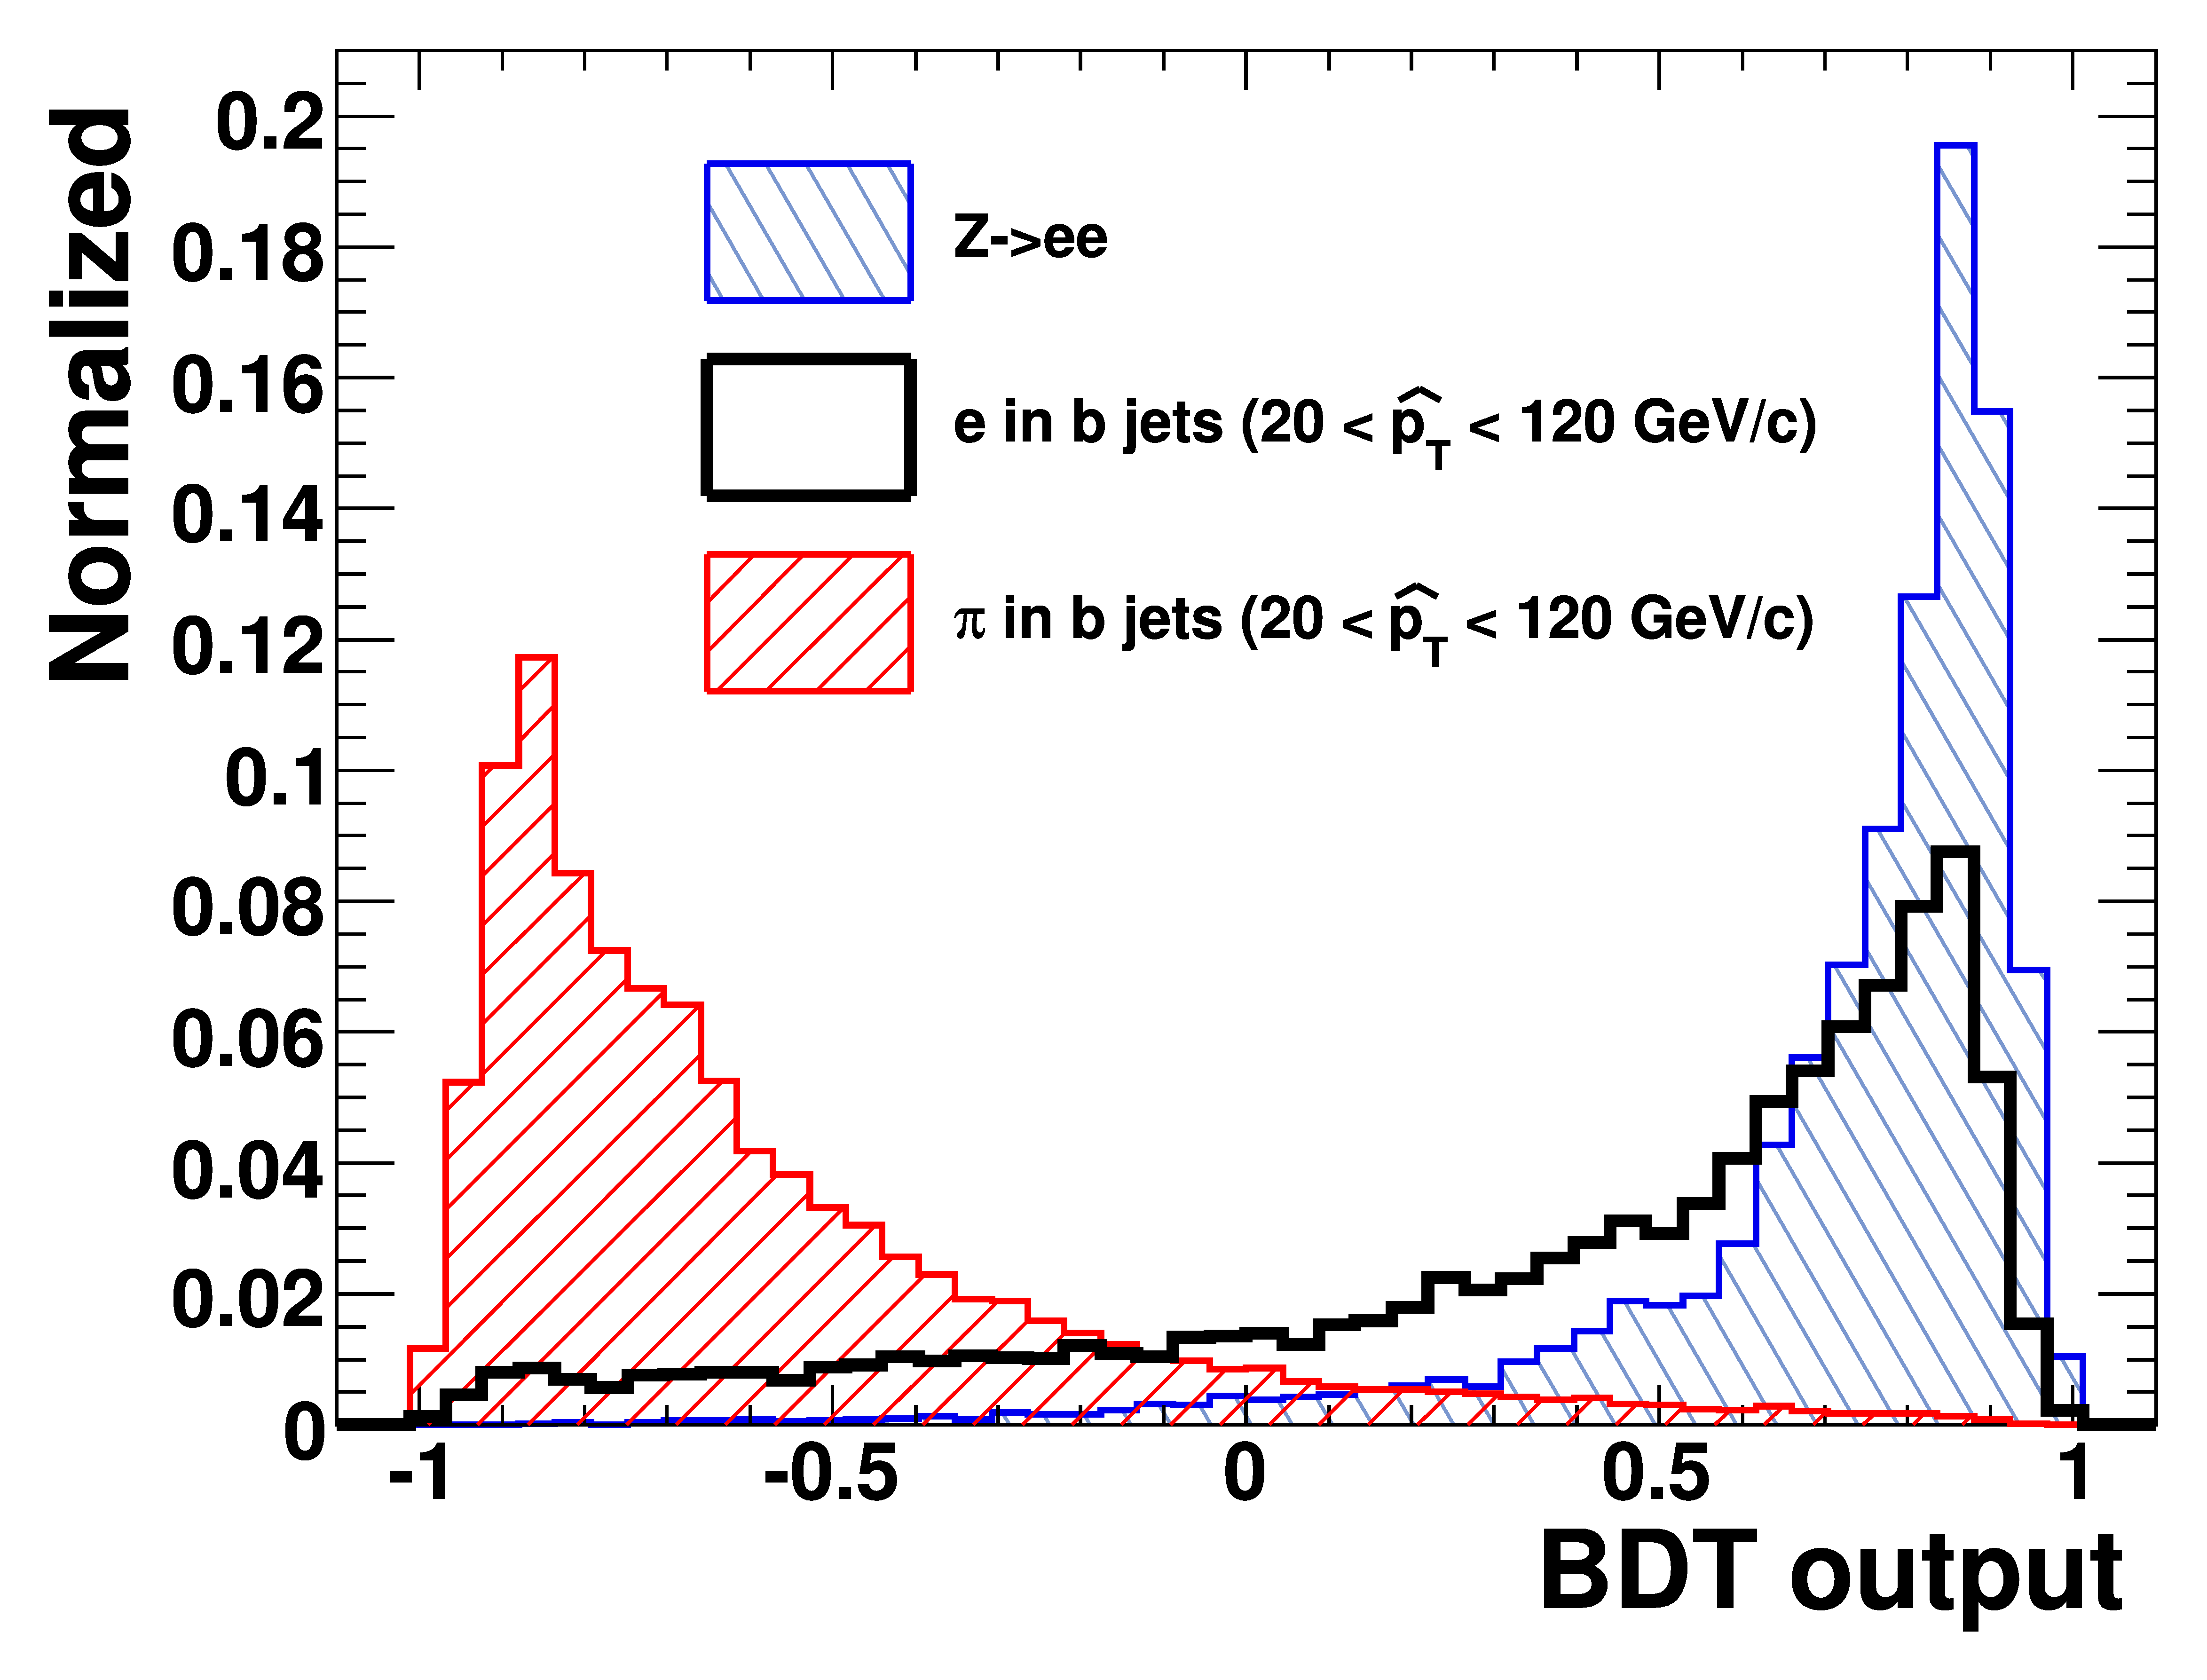
\includegraphics[width=0.5\textwidth]{chapitre3/figs/bdt_electron.pdf}} \hfill
    \subcaptionbox{\label{fig:jspi_ee}}[0.45\textwidth]{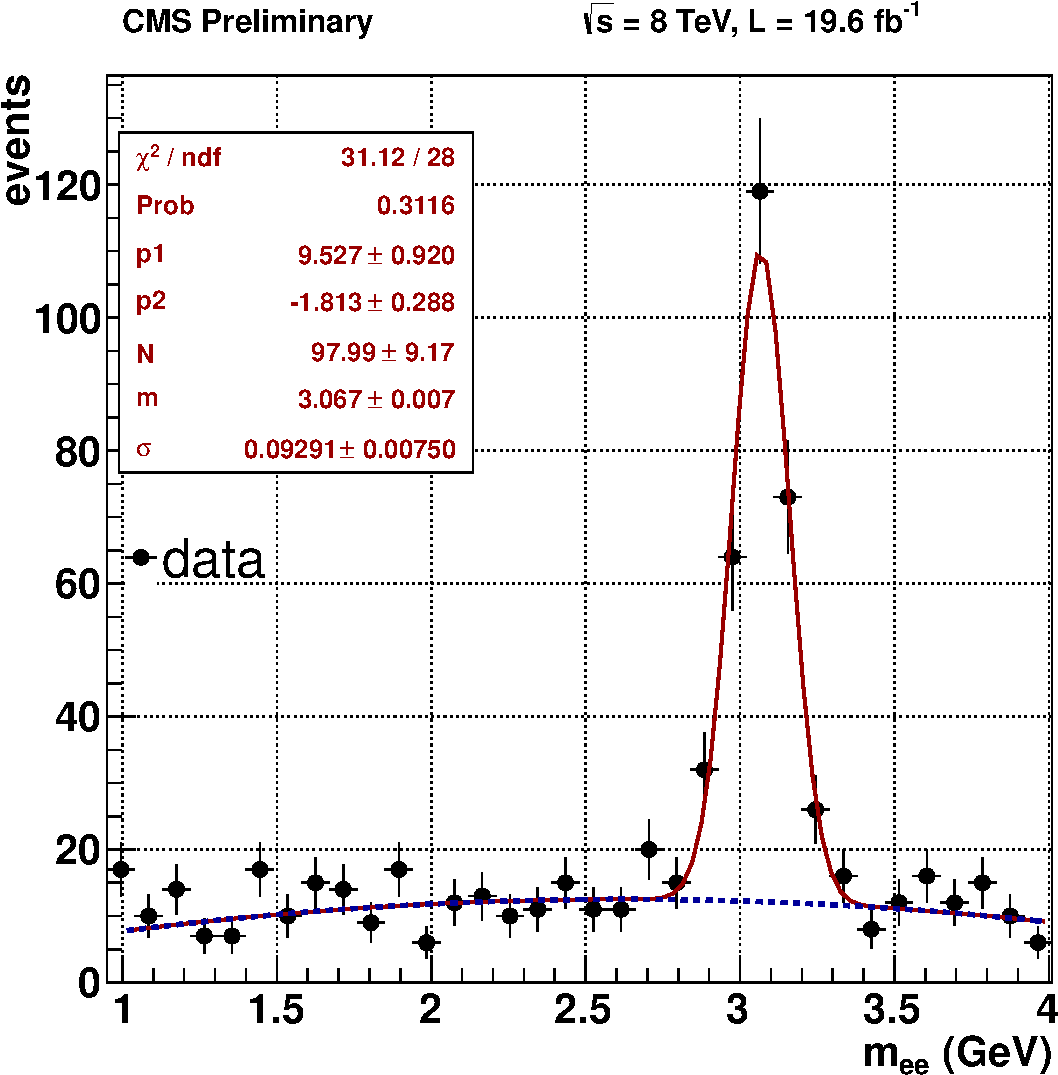
\includegraphics[width=0.45\textwidth]{chapitre3/figs/jspi_ee.pdf}}
    \caption{(\subref{fig:bdt_electron}) Sortie de l'algorithme de pré-sélection des électrons, pour des électrons isolés (bleu), des électrons dans des jets de $b$ (noir) et pour des pions dans des jets de $b$ \citep{pf}. (\subref{fig:jspi_ee}) Masse invariante di-électrons sur les données 2012 pour des événements $\PJpsi \rightarrow \Pelectron \Ppositron$ \citep{cms_electron_perf}.}
    \label{fig:electron_perf}
\end{figure}

La pré-sélection des électrons exploite les caractéristiques des traces. Lorsque la radiation Bremsstrahlung est négligeable, l'algorithme classique reconstruit une trace et on trouve un bloc \emph{particle-flow} associé. Si le rapport $E/p$ est proche de l'unité, la trace est sélectionnée. Lorsque le rayonnement Bremsstrahlung n'est pas négligeable, deux effets sont possibles :
\begin{itemize}
    \item L'algorithme de reconnaissance de traces échoue lors d'un changement abrupt de trajectoire. La trace résultante contient alors un petit nombre de \emph{hits}.
    \item L'algorithme de reconnaissance de traces reconstruit une trace, mais le $\chi^2$ associé est grand.
\end{itemize}

Une sélection est appliquée en utilisant le nombre de \emph{hits} et le $\chi^2$, puis une interpolation GSF (avec seulement 5 paramètres libres, donc moins contraignante) est effectuée si la trace passe la sélection. Le $\chi^2$ de cette interpolation ($\chi^2_{GSF}$), le rapport $\chi^2_{KF} / \chi^2_{GSF}$, le nombre de \emph{hits} ainsi que le facteur de qualité du lien ECAL -- trace sont utilisés en entrée d'un algorithme d'arbres de décision boosté. La sortie de cet algorithme est présentée \cref{fig:bdt_electron}. On peut voir l'excellente discrimination entre les électrons isolés et les pions, et la bonne séparation entre les électrons non isolés et les pions. Les performances de reconstruction des électrons sont évaluées sur des événements \PJpsi $\rightarrow \Pelectron \APelectron$ (\cref{fig:jspi_ee}). On obtient une résolution de reconstruction $\sigma = \SI{93}{\MeV}$.

On considère le candidat comme un électron si la sortie de l'algorithme est supérieure à \num{-0.1} \citep{cms_pf_electrons}. Dans ce cas, les blocs \emph{particle-flow} sont retirés de la liste des blocs disponibles.

\subsubsection{Reconstruction des hadrons et des photons}

A ce stade, il ne reste plus que les blocs \emph{particle-flow} correspondants aux hadrons (chargés ou neutres), ainsi qu'aux photons. Avant d'entamer la reconstruction, il convient de simplifier un peu les liens créés par l'algorithme de liaison. Si une trace est liée à plusieurs agrégats dans le HCAL, seul le lien ayant la plus petite distance ($\Delta R$, voir \cref{sec:pf_links}) est gardée. On procède de façon identique pour les liens dans le ECAL.

Dans de très rares cas, l'énergie des agrégats calorimétriques liés à une trace peut être très inférieure à l'impulsion de celle-ci. Si cette différence est supérieure à $3\sigma$, cela est probablement le signe de la présence d'un muon, ou d'une fausse trace. Un algorithme spécialisé, basé sur le même principe que celui servant à reconstruire les muons, mais avec des contraintes relâchées, permet d'identifier ces muons. S'il s'avère qu'aucun muon n'est présent, la trace est considérée comme fausse et est supprimée des blocs \emph{particle-flow}. Moins de \SI{0.3}{‰} des traces sont concernées par cette procédure.

Chaque trace restante donne lieu à la création de hadrons chargés \emph{particle-flow}, dont l'impulsion et l'énergie sont mesurées directement depuis la trace, selon l'hypothèse d'un pion chargé. Deux cas sont possibles :
\begin{itemize}
    \item L'énergie des agrégats calorimétriques liés à cette trace est compatible avec l'impulsion mesurée par la trace (dans les incertitudes). L'impulsion du hadron chargé est alors améliorée en combinant les informations de la trace et des agrégats calorimétriques, grâce à une moyenne pondérée. Cette combinaison est surtout intéressante à très haute énergie / très haut \aeta, où les paramètres des traces sont mesurés avec une grande incertitude.
    \item L'énergie des agrégats calorimétriques est plus grande que l'impulsion de la trace liée. C'est le cas si des photons ou des hadrons neutres, ne laissant pas de traces dans le trajectographe, ont déposé leur énergie au même endroit. Il faut donc réussir à correctement associer l'énergie avec les bonnes particules.

    \smallskip

    Si l'excès d'énergie ($E_\text{agrégats} - p_\text{trace}$) est supérieur à l'énergie déposée dans le ECAL ($E_E$), deux particules sont reconstruites : on assigne l'énergie du ECAL à un photon \emph{particle-flow}, et le restant de l'excès ($E_\text{HCAL} - p_\text{trace}$) à un hadron neutre \emph{particle-flow}. Dans le cas contraire, seul un photon \emph{particle-flow} est reconstruit avec l'excès d'énergie. La priorité donnée aux photons sur les hadrons neutres dans le ECAL est justifiée par l'observation que seul environ \SI{3}{\%} de l'énergie des hadrons neutres est déposée dans le calorimètre électromagnétique.
\end{itemize}

Enfin, les blocs \emph{particle-flow} restant n'ont aucune trace liée. On reconstruit avec les agrégats dans le ECAL les photons \emph{particle-flow}, et avec ceux dans le HCAL les hadrons neutres \emph{particle-flow}.

\begin{figure}[tbp]
    \centering
    \subcaptionbox{\label{fig:mgg}}[0.55\textwidth]{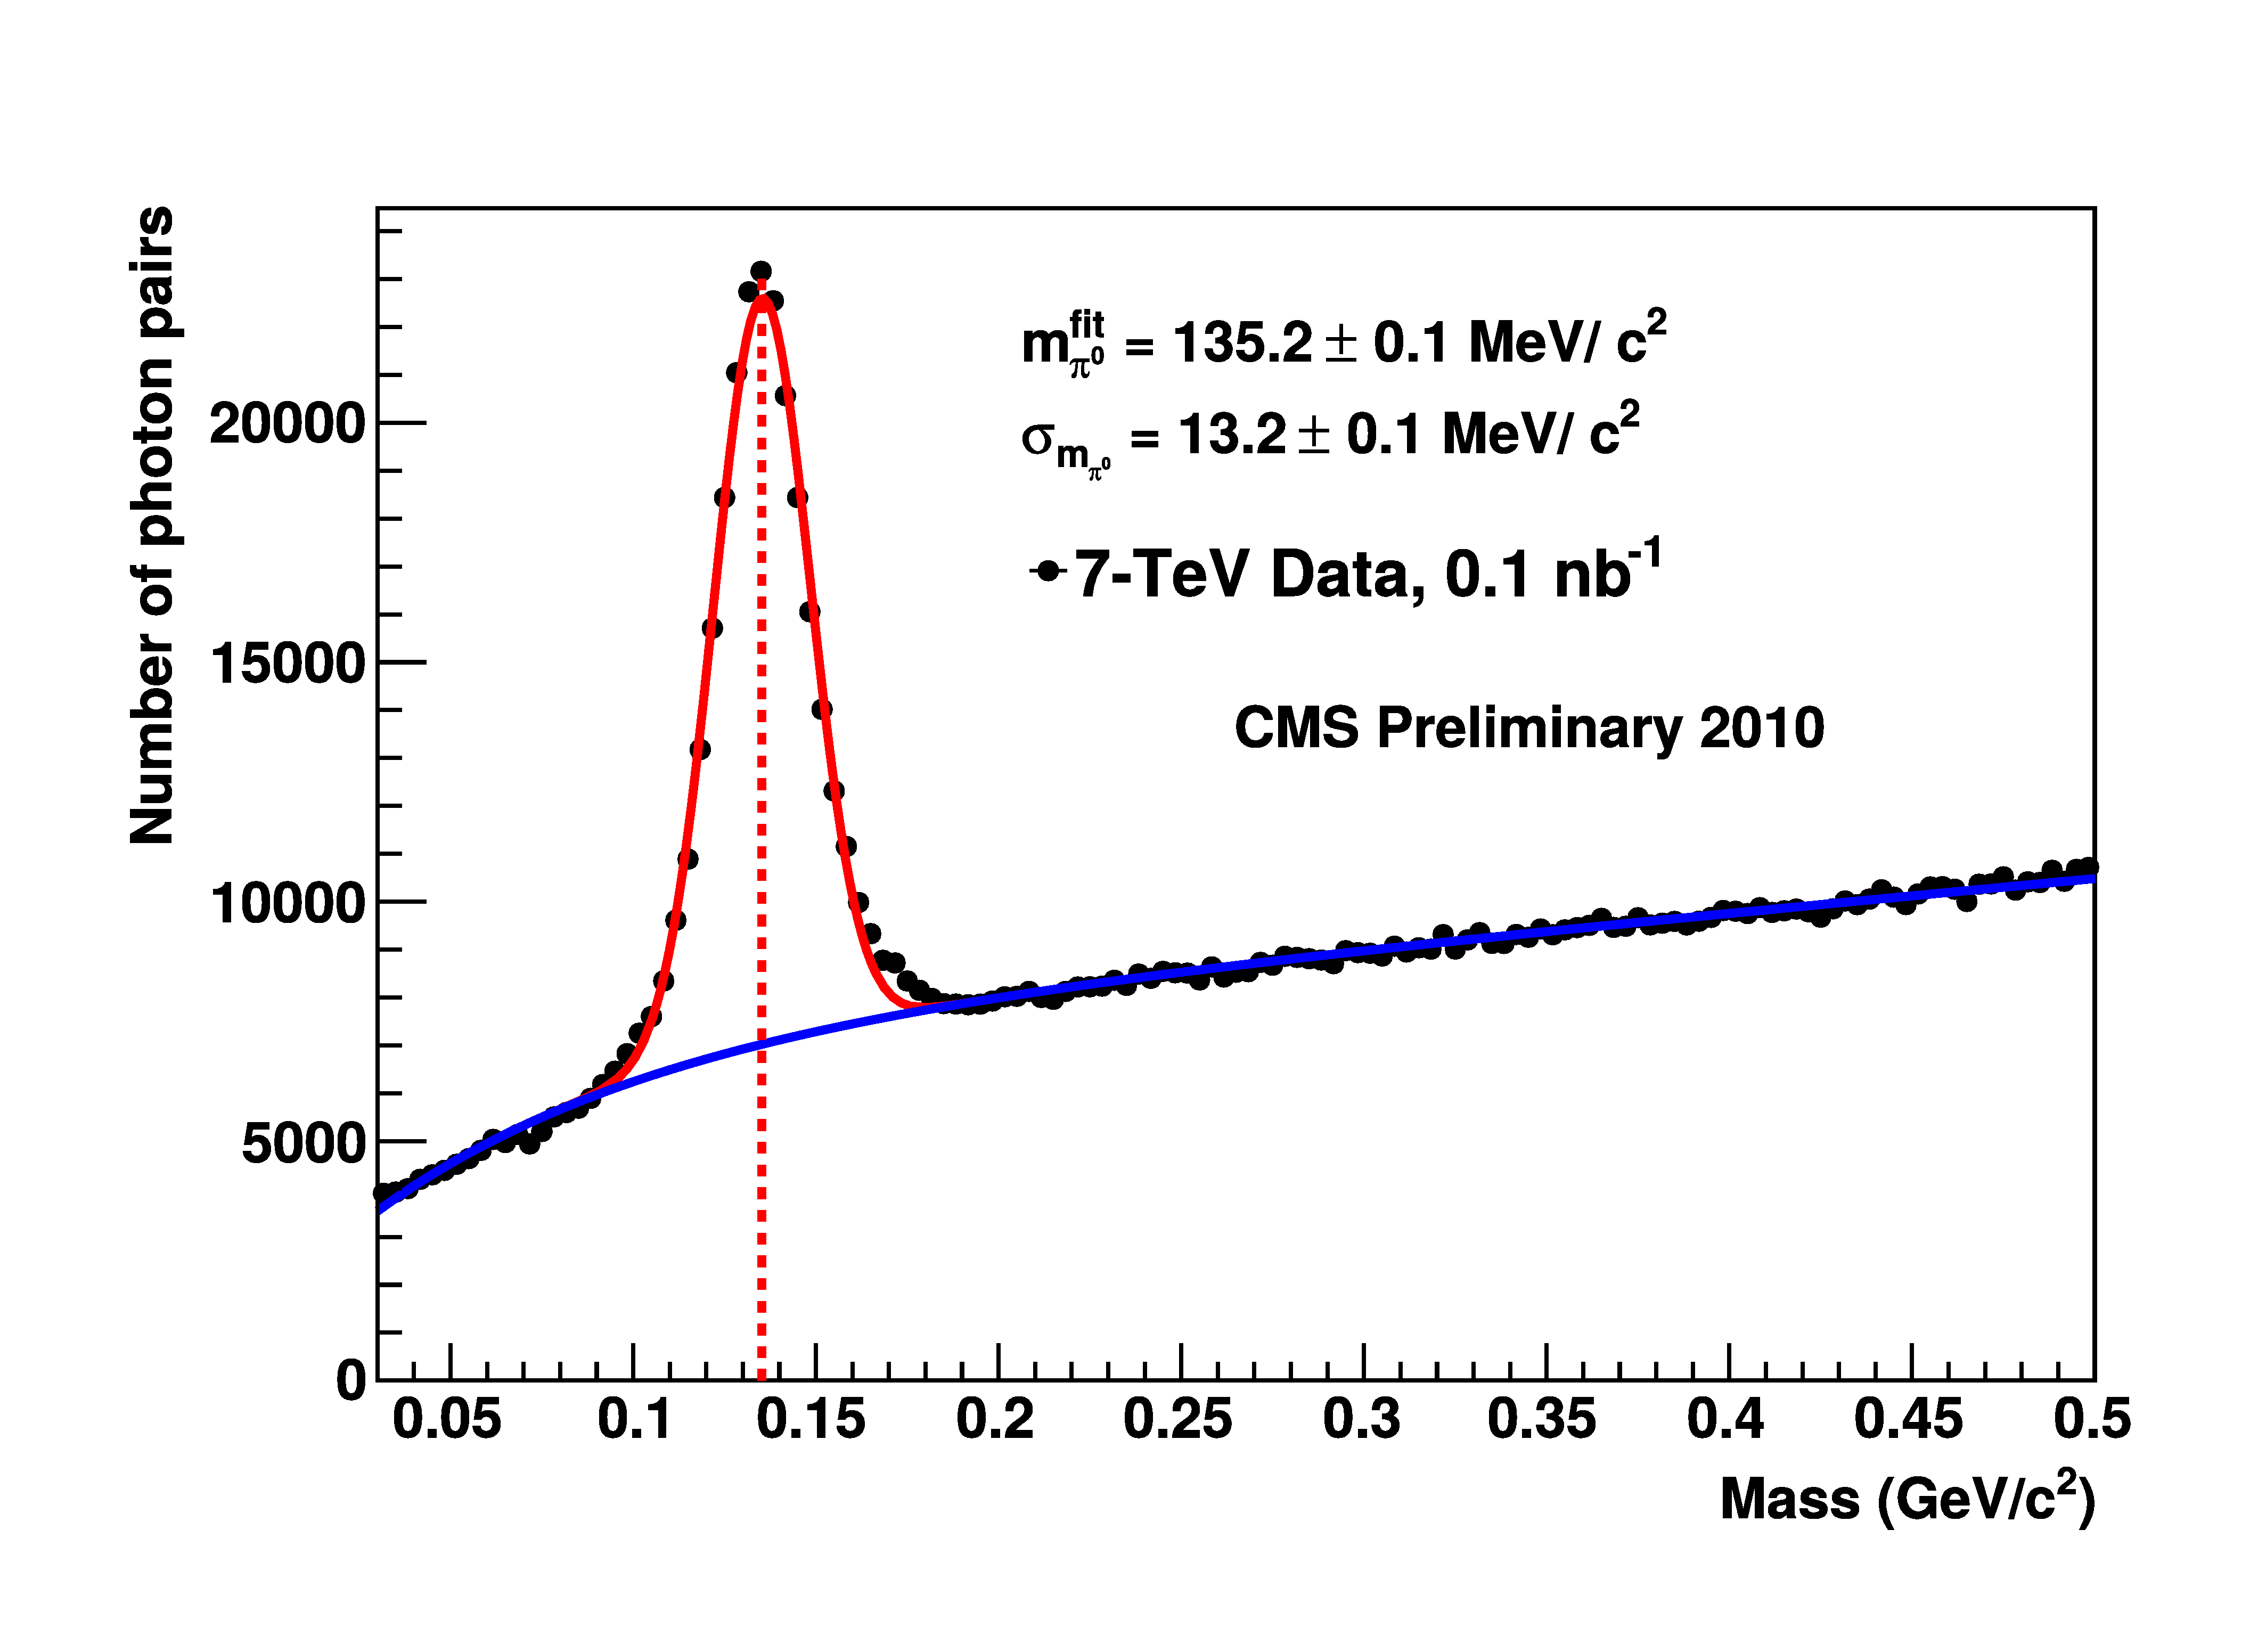
\includegraphics[width=0.55\textwidth]{chapitre3/figs/pf_photons.pdf}} \hfill
    \subcaptionbox{\label{fig:gamma_eff}}[0.44\textwidth]{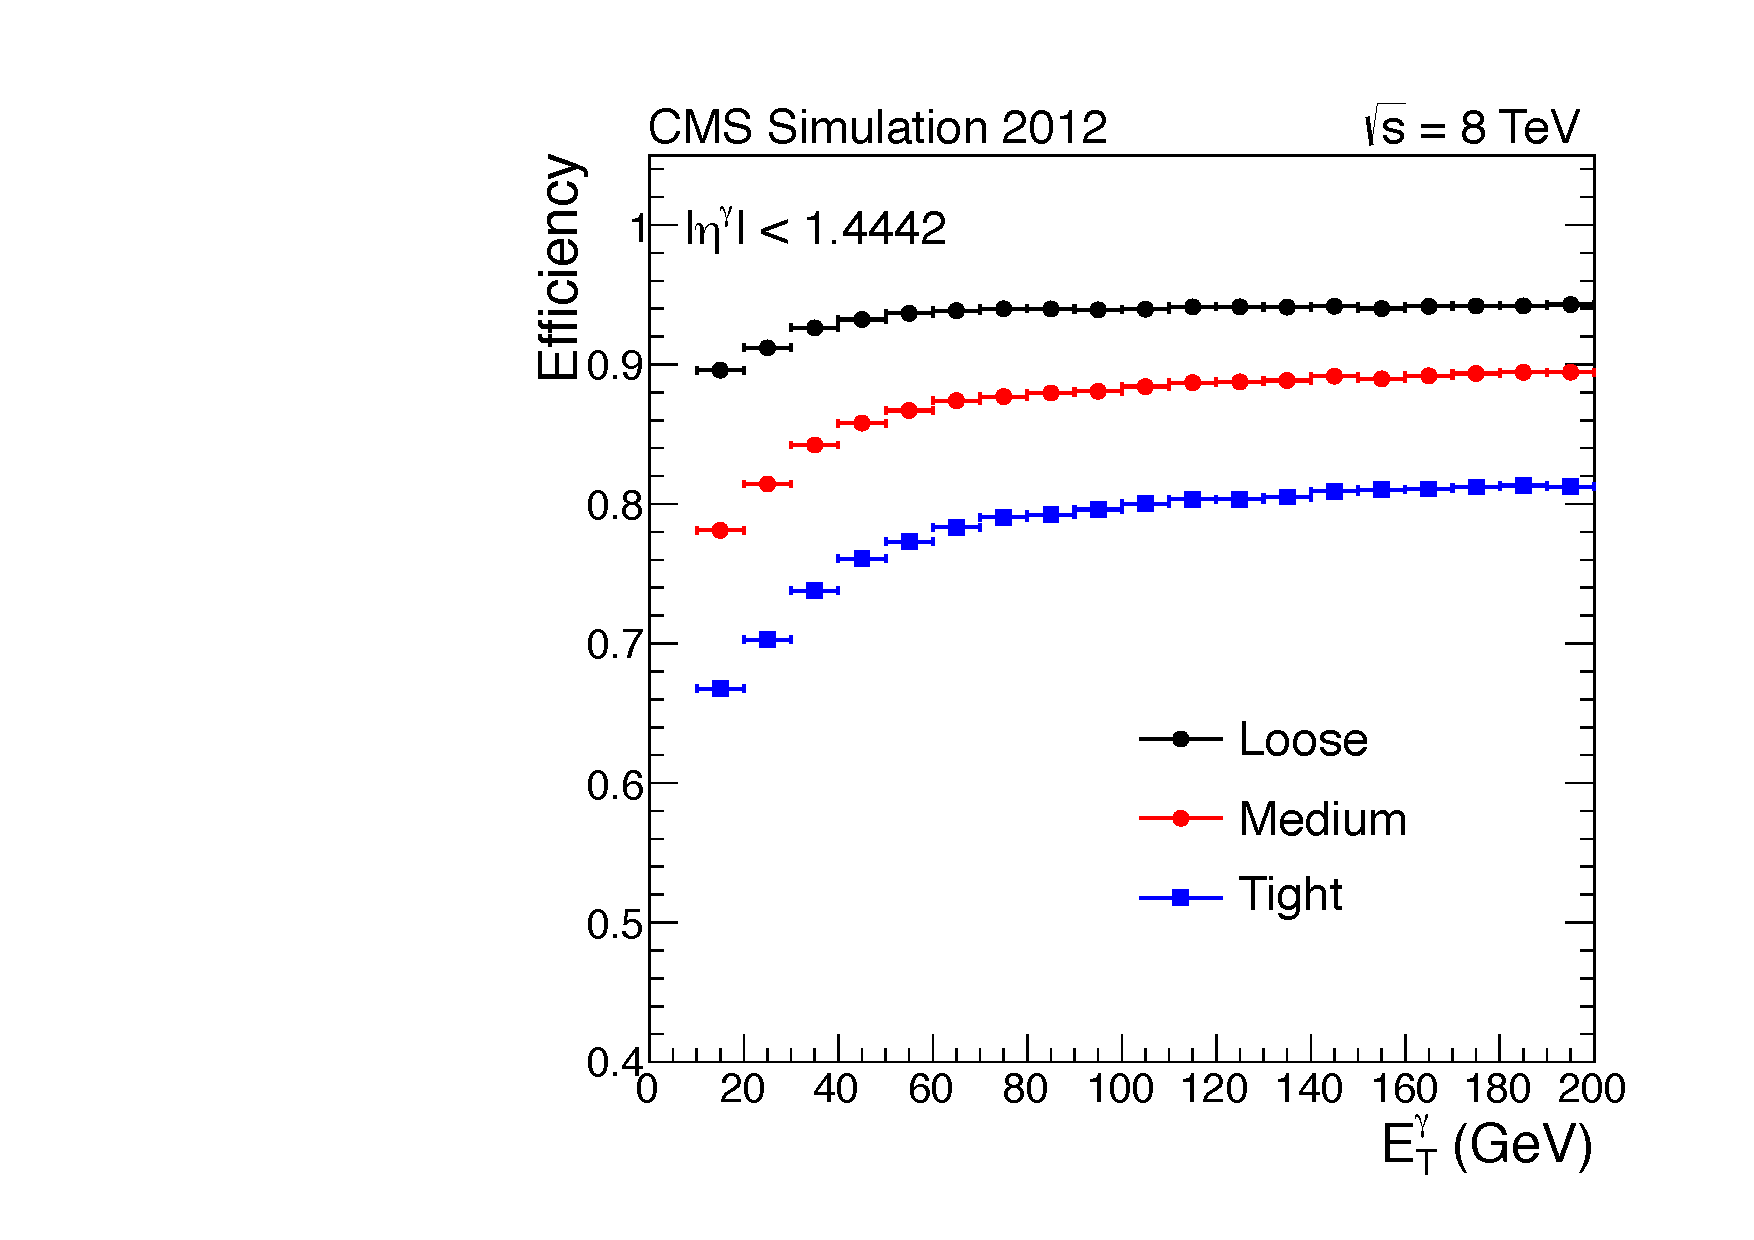
\includegraphics[width=0.44\textwidth]{chapitre3/figs/photon_eff.pdf}}
    \caption{(\subref{fig:mgg}) Distribution de la masse invariante $\gamma\gamma$ dans le tonneau obtenu à l'aide des données 2010, grâce à une sélection optimisée pour les $\pi^0$. Le désaccord avec la mesure de la masse du $\pi^0 = \SI{135}{\MeV}$ est inférieur à \SI{1}{\%}. \citep{cms_pf_jets}. (\subref{fig:gamma_eff}) Efficacité d'identification des photons pour les trois points de fonctionnement recommandés par CMS \citep{cms_photon_perf}.}
    \label{fig:pf_photons}
\end{figure}

On présente \cref{fig:mgg} la résolution expérimentale obtenue lors de la reconstruction d'événement $\Ppizero \rightarrow \Pgamma \Pgamma$. On trouve une résolution $\sigma = \SI{13}{\MeV}$. L'efficacité d'identification pour les trois points de fonctionnement définis par la collaboration CMS est présentée \cref{fig:gamma_eff}. Dans tous les cas, cette efficacité est supérieure à \SI{65}{\%}.

\subsubsection{Isolation des leptons} \label{sec:lepton_isolation}

Bien souvent, il est important pour les analyses de physique de savoir si un lepton est isolé, c'est-à-dire de savoir si l'activité autour du lepton est faible. L'isolation du lepton est définie par la relation
\begin{align*}
  I_{\Plepton} &= \frac{\sum{\pt^\text{hadrons chargés}} + \sum{\pt^\text{hadrons neutres}} + \sum{\pt^\text{photons}}}{\pt^{\Plepton}}
\end{align*}
où les sommes portent sur les particules contenues dans un cône de rayon $\Delta R$ centré autour du lepton. Ainsi, plus $I$ tend vers 0, plus la particule est isolée. Deux valeurs de $\Delta R$ sont utilisées, suivant la saveur du lepton :
\begin{align*}
  \Delta R &= \num{0.4} \quad\text{muons}\\
  \Delta R &= \num{0.3} \quad\text{électrons}
\end{align*}

Dans le cas des muons, la définition de l'isolation $I$ est modifiée afin d'être plus robuste face au \pu. On considère en effet les hadrons chargés provenant d'un vertex autre que le vertex principal comme du \pu : ils ne sont donc pas utilisés dans le calcul de l'isolation. Ce n'est malheureusement pas suffisant, puisque le \pu est aussi composé de hadrons neutres et de photons : on estime que ces hadrons sont responsables d'environ la moitié de l'énergie du \pu. Ainsi, on soustrait du calcul de l'isolation la moitié de l'énergie des hadrons identifiés comme provenant du \pu, en vérifiant bien que l'énergie provenant de la partie neutre ne soit jamais négative. On obtient alors
\begin{align*}
  I_{\Pmu}^\text{corrigé} &= \frac{\sum{\pt^\text{hadrons chargés}} + \overbrace{\left(\sum{\pt^\text{hadrons neutres}} + \sum{\pt^\text{photons}} - \num{0.5} \sum{\pt^\text{hadrons chargés \pu}} \right)}^{= 0 \text{ si négatif}}}{\pt^{\Plepton}}
\end{align*}
On considère un muon comme isolé si $I_{\Pmu}^\text{corrigé} < \SI{12}{\%}$.

\smallskip

Pour les électrons, on applique une procédure similaire. Néanmoins, au lieu de soustraire la moitié de l'énergie des hadrons chargés provenant du \pu, on estime l'énergie restant due au \pu en utilisant la densité d'énergie dans l'événement par unité de surface ($\rho$, voir \cref{sec:jec_l1}). Au lieu d'utiliser la surface du cône d'isolation, parfois délicate à calculer géométriquement, pour estimer la quantité d'énergie du \pu, on évalue une surface effective ($EA$) sur des événements \PZ $\rightarrow$ \Pelectron{}\Ppositron.% Cette surface est définie comme le rapport entre la pente de la droite $\rho = f(N_{\text{vertex}})$ et la pente de la droite $I = f(N_\text{vertex})$. \fxnote{Revoir la partie sur EA.}
\begin{align*}
  I_{\Pe}^\text{corrigé} &= \frac{\sum{\pt^\text{hadrons chargés}} + \overbrace{\left(\sum{\pt^\text{hadrons neutres}} + \sum{\pt^\text{photons}} - \rho\,EA \right)}^{= 0 \text{ si négatif}}}{\pt^{\Plepton}}
\end{align*}
On considère un électron comme isolé si $I_{\Pe}^\text{corrigé} < \SI{10}{\%}$. Cette valeur est plus faible en raison de la taille du cône plus faible également.

\subsection{Calibration des calorimètres}

\begin{figure}[tbp]
    \centering
    \subcaptionbox{\label{fig:hadron_calib_barrel}}[0.48\textwidth]{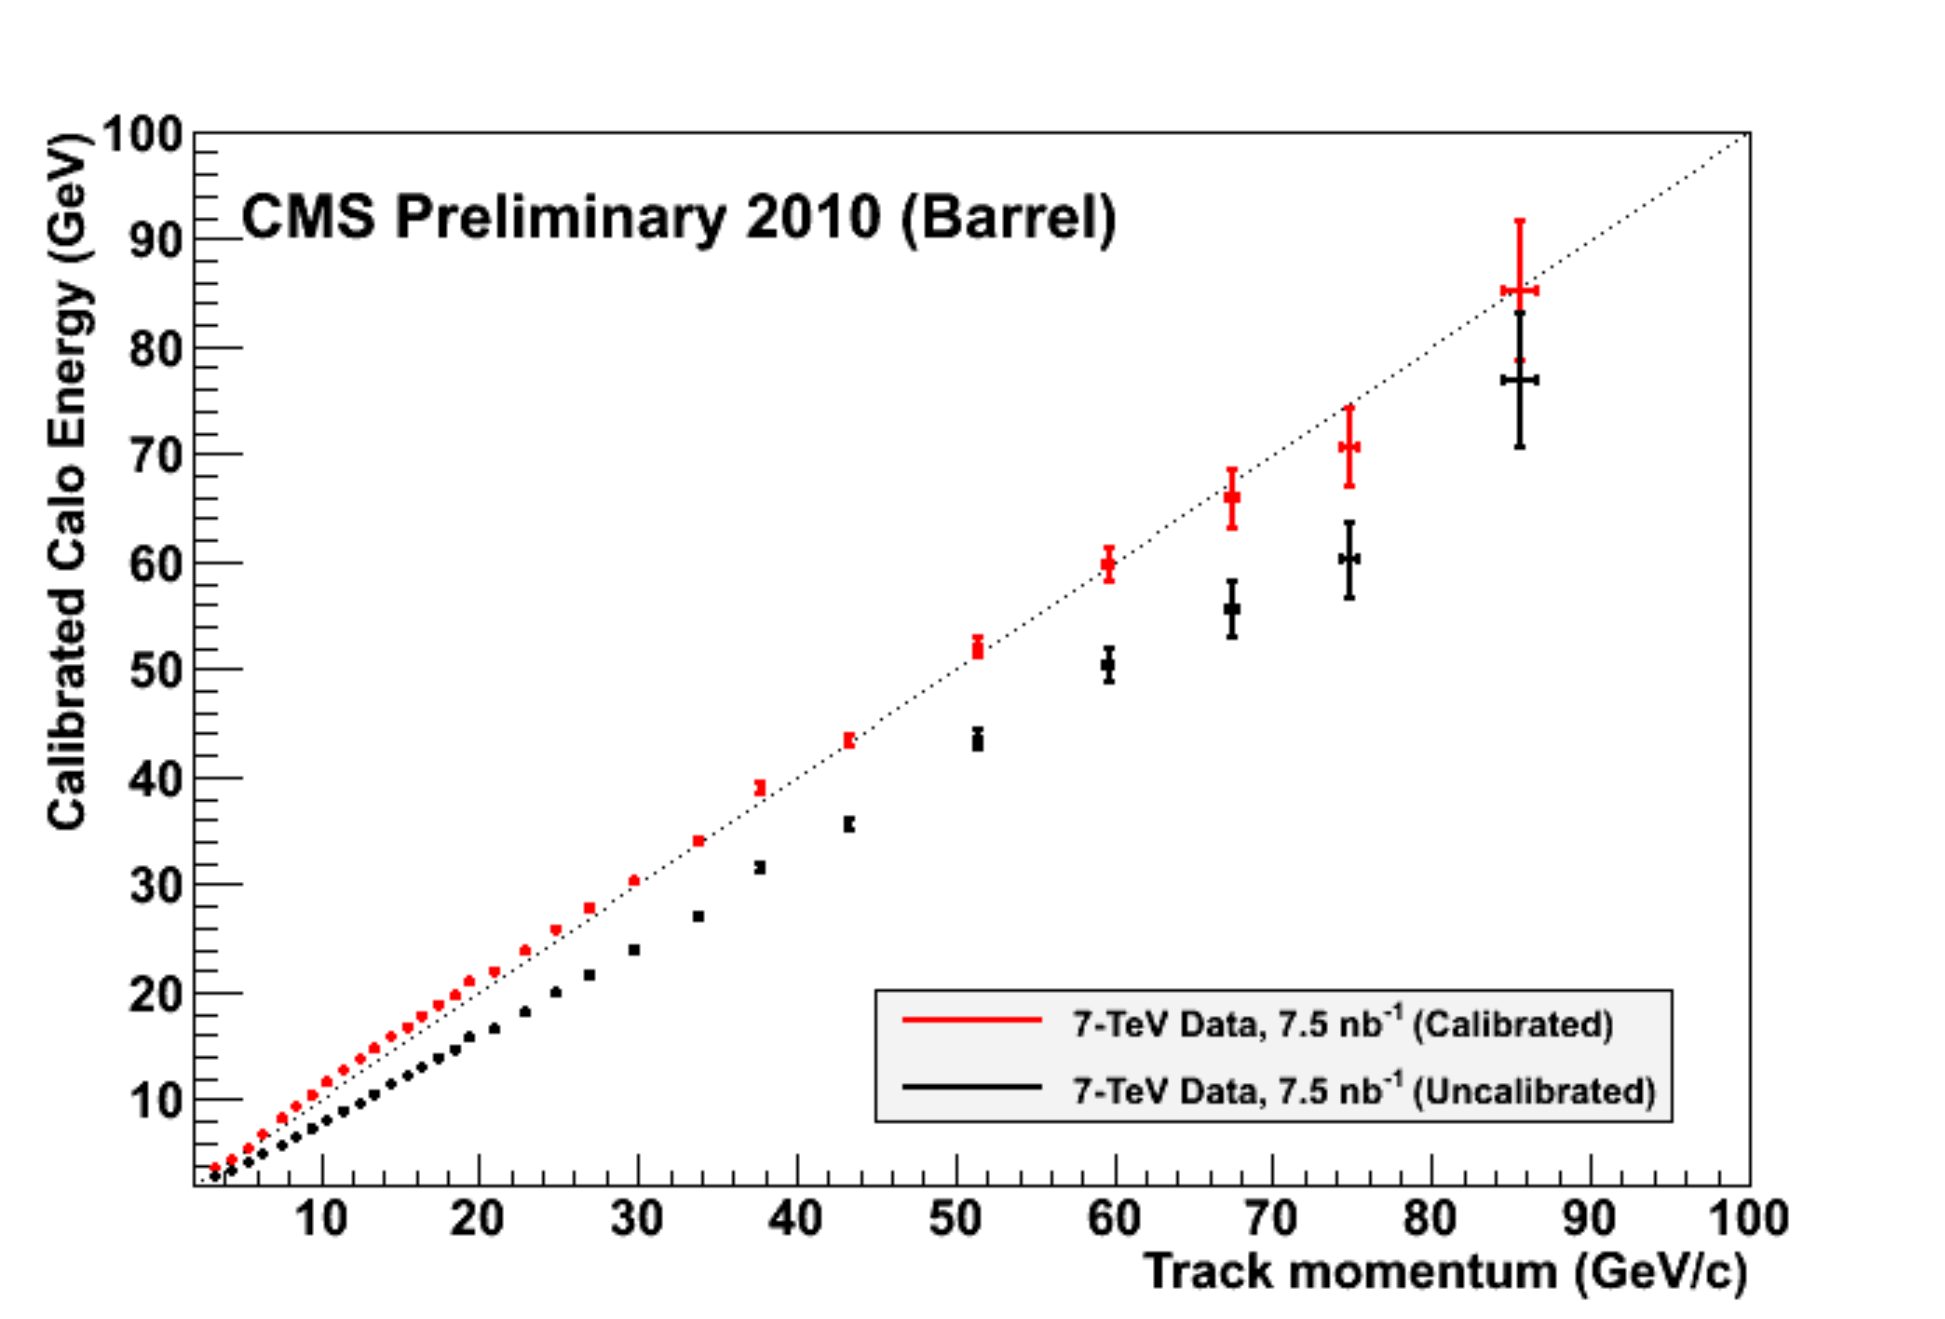
\includegraphics[width=0.48\textwidth]{chapitre3/figs/hadron_calib_barrel.png}} \hfill
    \subcaptionbox{\label{fig:hadron_calib_endcap}}[0.48\textwidth]{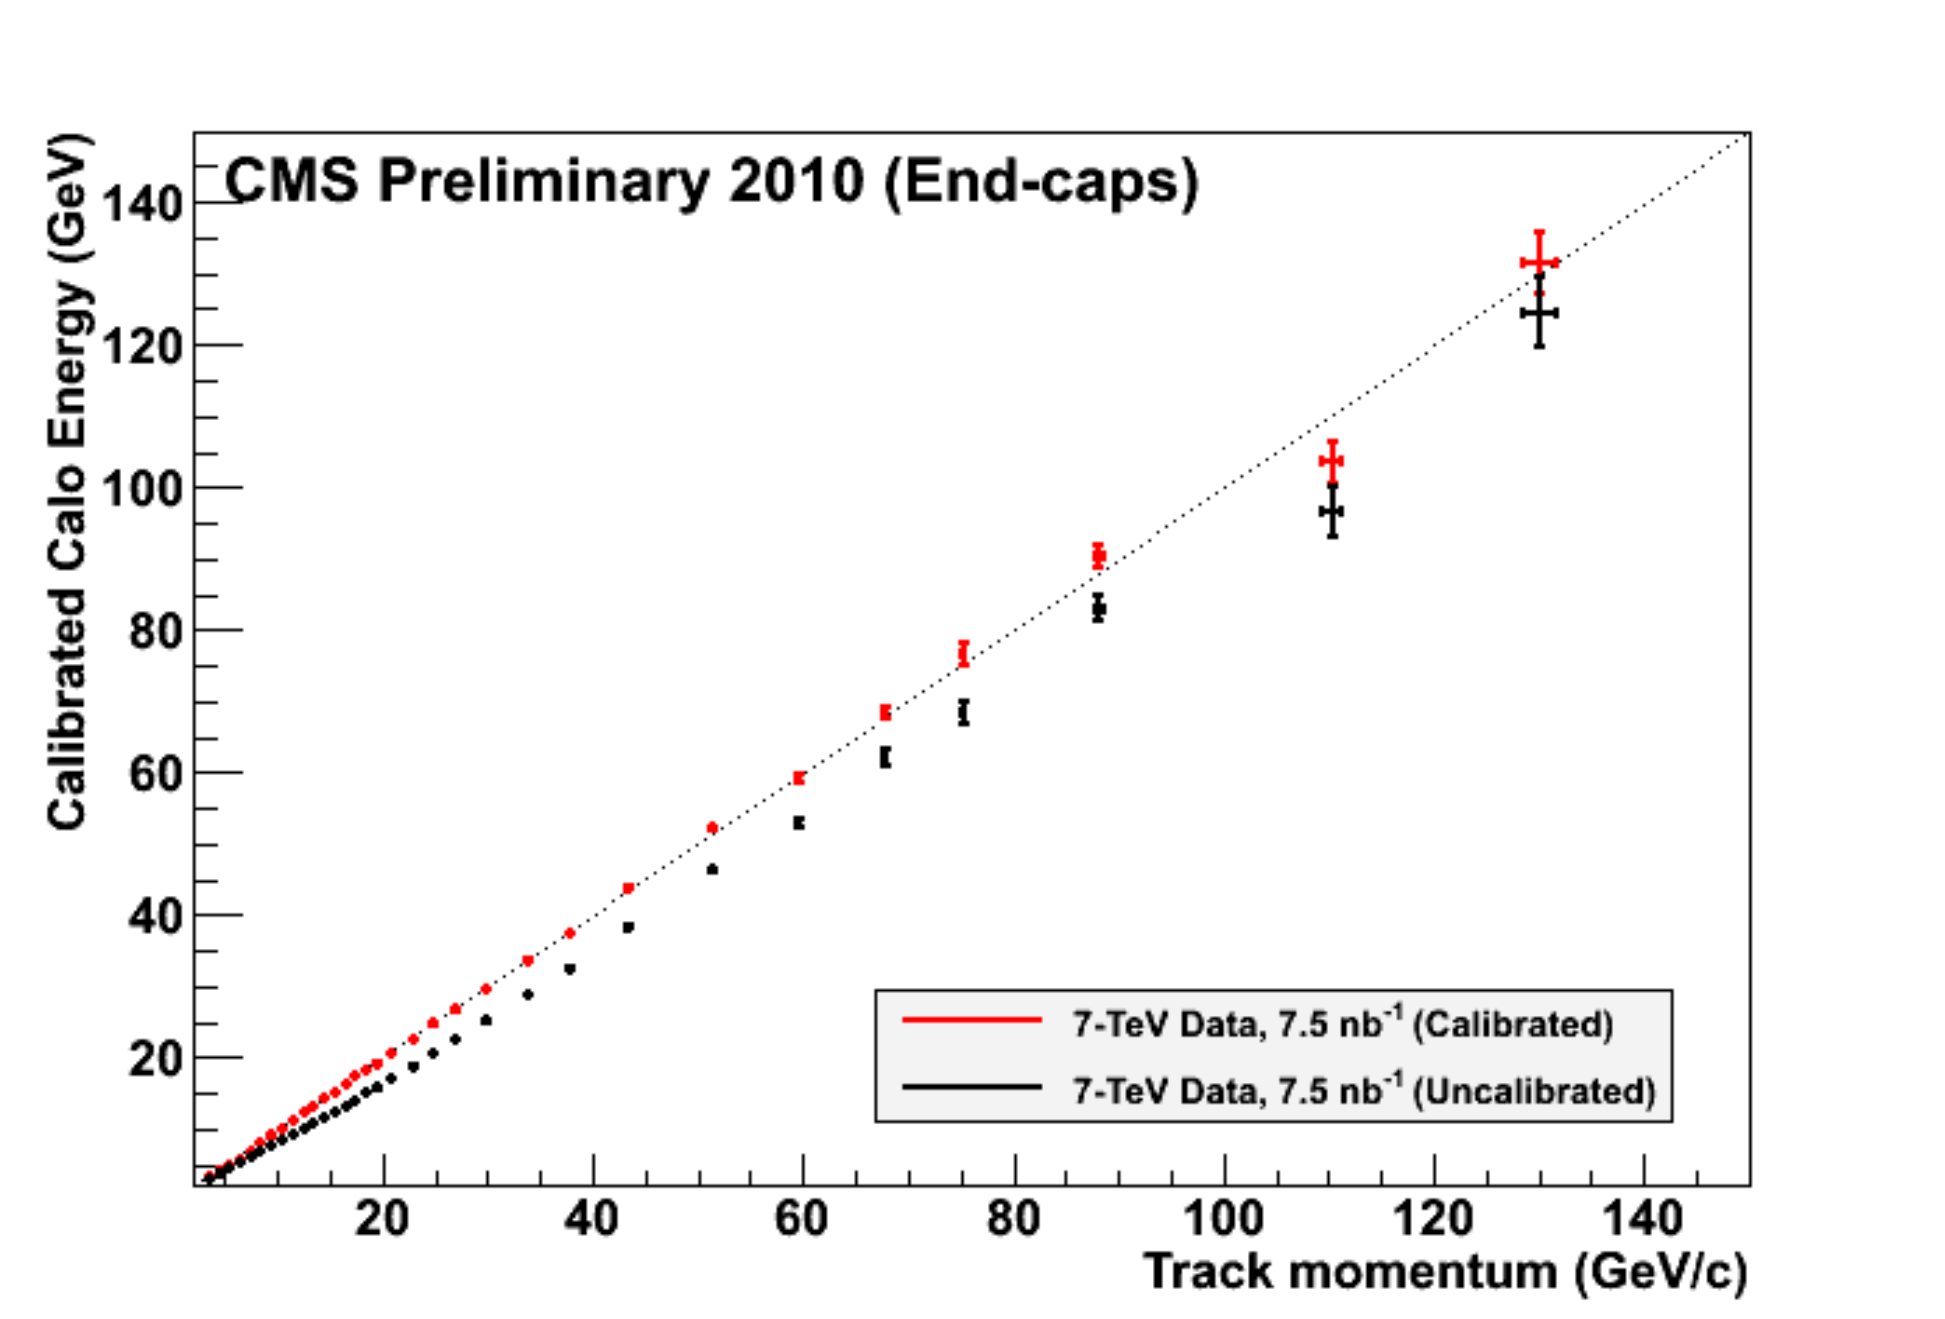
\includegraphics[width=0.48\textwidth]{chapitre3/figs/hadron_calib_endcap.png}}
    \caption{Effet de la calibration de l'énergie des hadrons chargés dans le tonneau (\subref{fig:hadron_calib_barrel}) et dans les bouchons (\subref{fig:hadron_calib_endcap}).}
    \label{fig:hadron_calib}
\end{figure}

Afin d'estimer au mieux l'énergie des particules reconstruites, les calorimètres doivent être calibrés en fonction du type de particules reconstruites. Par exemple, la réponse du calorimètre pour les photons ou les hadrons chargés n'est pas identique.

Pour les électrons et les photons, des corrections sont dérivées en utilisant la simulation comme référence, et en exploitant des processus physiques bien connus, tel que $\PZ \rightarrow \Pelectron \Ppositron$ pour la calibration des électrons ou $\PZ \rightarrow \Pmuon \APmuon \Pphoton$ pour la calibration des photons.

Pour les hadrons chargés, l'énergie calorimétrique associée au bloc \emph{particle-flow} est calibrée par la fonction
\begin{align*}
  E_\text{calib} &= a + b\left(E, \eta\right) E_\text{ECAL} + c\left(E, \eta\right)E_\text{HCAL}
\end{align*}
où $a$, $b$, $c$ sont des constantes de calibration à déterminer, $E$ l'énergie totale non calibrée du hadron chargé, et $\eta$ la pseudo-rapidité de la cellule du HCAL. Ces constantes ont été déterminées sur les premières données en 2010. On peut voir \cref{fig:hadron_calib} l'effet de la calibration sur la détermination de l'énergie des hadrons chargés. Cette calibration impacte directement la mesure de l'énergie des photons et des hadrons neutres. Elle est donc primordiale.

\subsection{Reconstruction des jets} \label{sec:jet_reco}

% \begin{figure}[tbp]
%     \centering
%     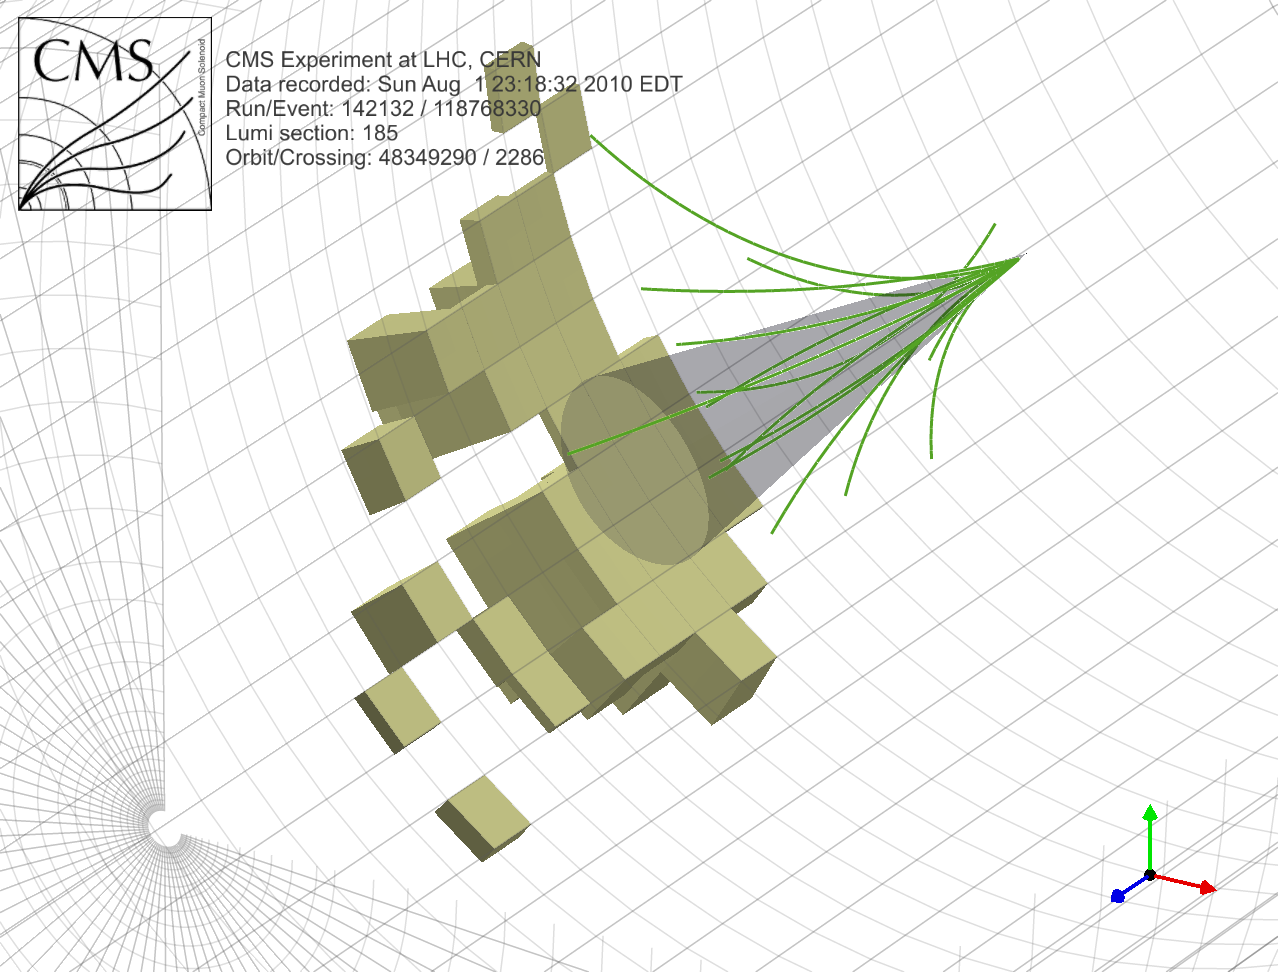
\includegraphics[width=0.5\textwidth]{chapitre3/figs/jet.png}
%     \caption{Reconstruction d'un jet dans CMS. Les traces et les dépôts calorimétriques ont été rendus visible.}
%     \label{fig:jet}
% \end{figure}

A cause du confinement lié à l'interaction forte, les quarks et gluons produits lors des collisions ne peuvent pas être observés directement. En effet, lors de leurs propagations, ils vont se combiner avec d'autre quarks pour former des hadrons. On obtient alors une cascade d'hadronisation, et on détecte ainsi une gerbe de particules en lieu et place d'un quark. Cette gerbe de particules, formées principalement de hadrons, mais aussi de leptons, est appelée \emph{jet}. %On peut voir \cref{fig:jet} la reconstruction d'un jet dans CMS. On voit bien une grande quantité de traces, associées à l'hadronisation d'un quark ou d'un gluon.

Grâce à l'algorithme de \emph{particle-flow}, on dispose d'une description globale de l'événement, sous forme d'une liste de particules. On utilise des algorithmes spécialisés qui vont parcourir la liste des particules, et former des agrégats suivant certains critères de distance entre les particules, différents selon les algorithmes. CMS utilise majoritairement deux types d'algorithmes : l'algorithme \emph{anti-$k_T$} \citep{antikt} et l'algorithme \emph{Cambridge-Aachen} (C-A) \citep{ca_jets}. Ce dernier est principalement utilisé lorsque l'on cherche une possible sous-structure au sein d'un jet. Par exemple, dans le cas de la désintégration d'un boson $W$ de très grande impulsion, les deux quarks peuvent être produits de façon très colinéaire, entraînant la reconstruction d'un seul gros jet, au lieu de deux.

Dans le but d'éviter d’agréger au sein d'un jet des leptons isolés, on commence par les supprimer de la liste des particules. On évite ainsi des doubles comptages de l'énergie, où un lepton pourrait se trouver dans une collection leptons mais aussi dans un jet. On définit l'isolation d'un lepton comme le rapport entre l'énergie des particules contenues dans un cône de rayon $\Delta R$, centré sur le lepton, sur l'énergie de ce lepton. En dessous d'un certain seuil (typiquement, \num{10} ou \SI{12}{\%}), on considère le lepton isolé.

\medskip

\begin{figure}[tbp]
    \centering
    \subcaptionbox{\label{fig:jets_akt}}[0.45\textwidth]{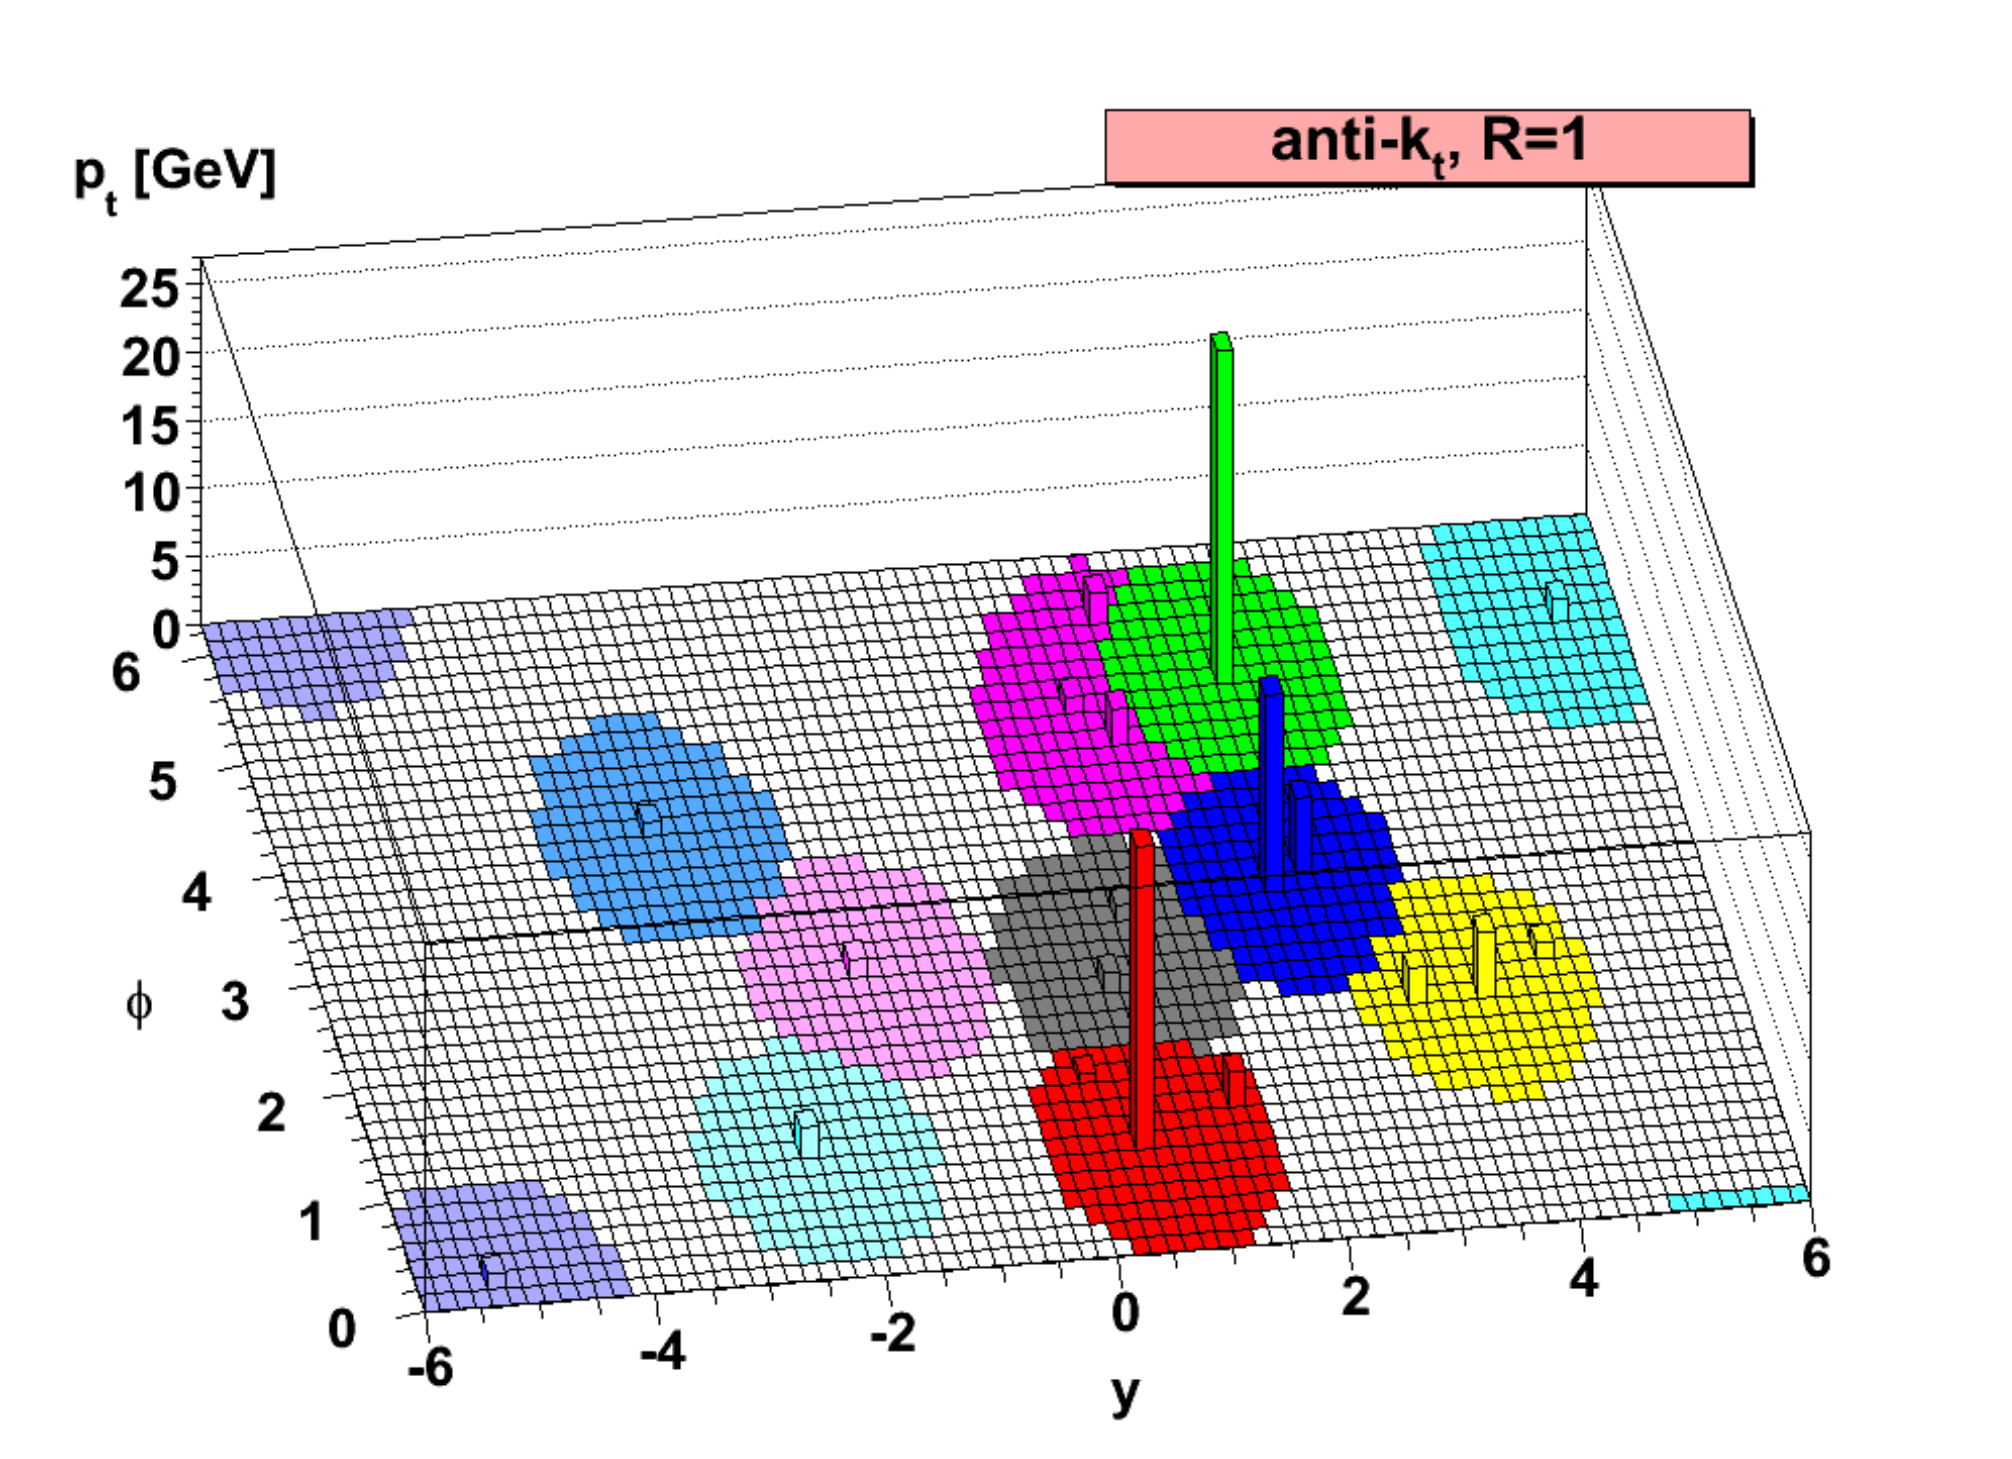
\includegraphics[width=0.45\textwidth]{chapitre3/figs/jets_akt.png}} \hfill
    \subcaptionbox{\label{fig:jets_ca}}[0.45\textwidth]{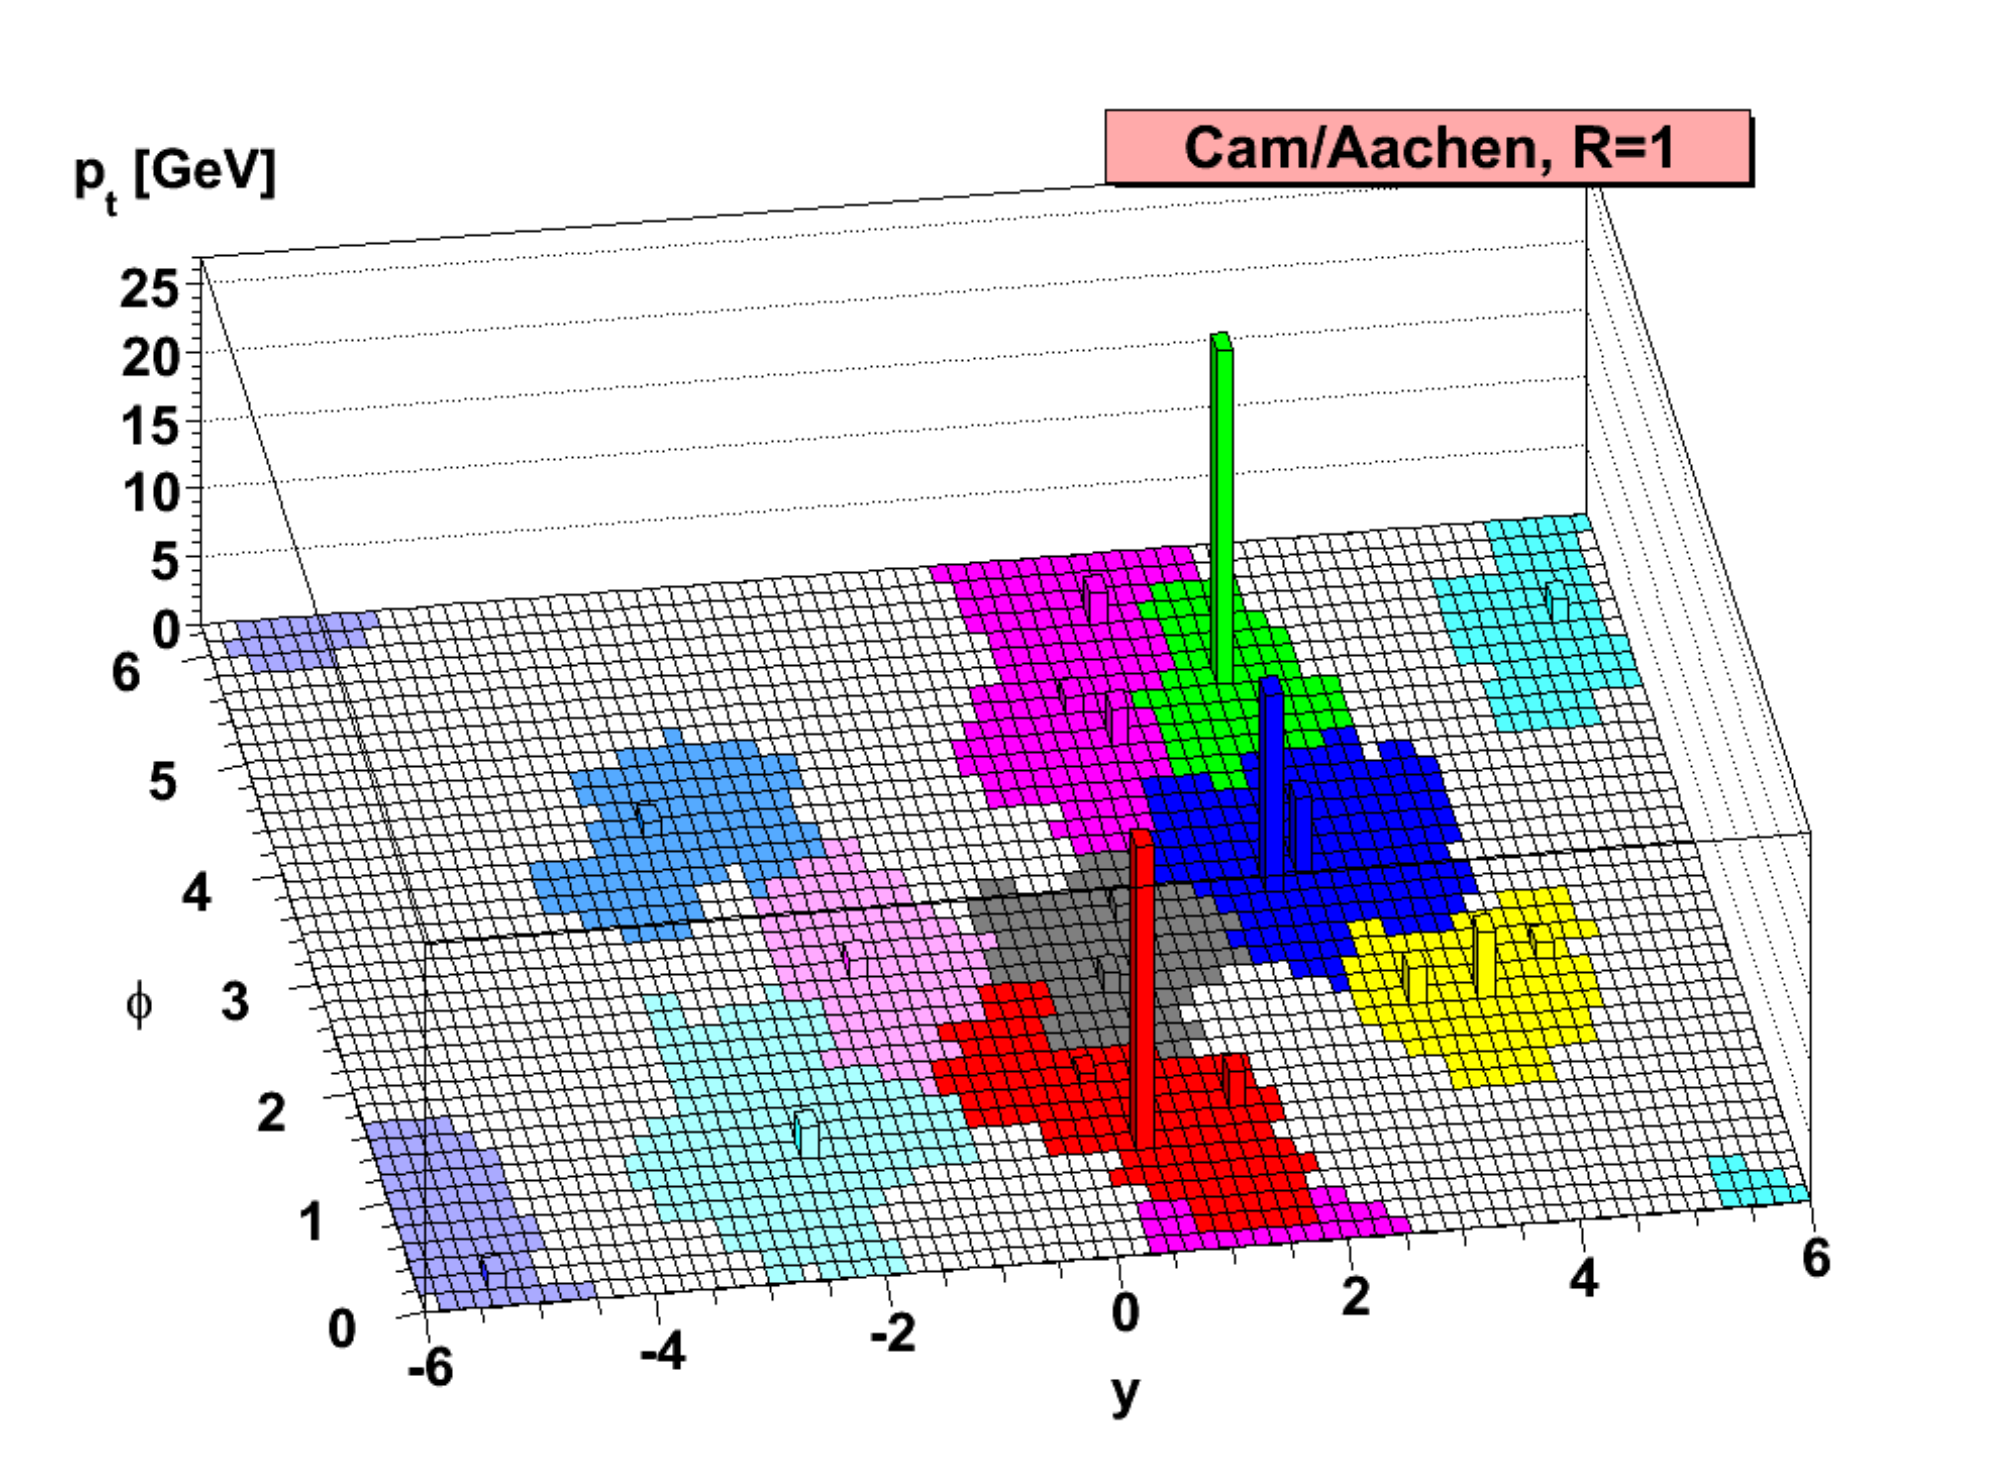
\includegraphics[width=0.45\textwidth]{chapitre3/figs/jets_ca.png}}
    \caption{Reconstruction des jets dans le plan ($\eta$, $\phi$) effectuée sur le même événement par l'algorithme anti-$k_T$ (\subref{fig:jets_akt}) et par l'algorithme C-A (\subref{fig:jets_ca}), pour une distance $R = 1$ \citep{antikt}.}
    \label{fig:akt_ca}
\end{figure}

Les deux algorithmes précédemment mentionnés itèrent sur la collection de particules, et tentent de construire un jet en associant les particules deux à deux. Pour ce faire, ils utilisent les quantités suivantes :
\begin{align*}
  d{ij} &= \text{min}\left( k_{T, i}^n, k_{T, j}^n \right) \frac{\Delta R^2_{ij}}{R^2} \\
  d_{iB} &= k^n_{T, i}
\end{align*}
où $k_{T, i}$ est l'impulsion transverse de la particule $i$ par rapport à l'axe du faisceau, $\Delta R_{ij}$ la distance entre $i$ et $j$ dans le plan ($\eta$, $\phi$), et $R$ une distance, choisie par l'utilisateur, symbolisant la largeur du jet. Pour l'algorithme \emph{anti-$k_T$}, on a $n = -2$, tandis que pour C-A, on a $n = 1$. $d_{iB}$ est un estimateur de la distance entre la particule $i$ et le faisceau.

L'algorithme cherche la valeur minimum $d_{min}$ entre tous les $d_{ij}$ et $d_{iB}$. Si le minimum est obtenu pour une valeur de $d_{ij}$, les particules $i$ et $j$ sont fusionnées (leurs quadrivecteurs sont sommés), et l'algorithme recommence. Au contraire, si le minimum est obtenu pour $d_iB$, la particule $i$ (souvent résultant de la fusion de plusieurs autres particules lors des itérations précédentes de l'algorithme) est considérée comme un jet et enlevée de la liste des particules. L'algorithme stoppe quand aucune particule ne reste.

La seule différence entre ces deux algorithmes vient de la façon dont le choix des particules à grouper est fait. Pour l'algorithme \emph{anti-$k_T$}, le poids de chaque paire est proportionnel à $\text{min}\left( 1 / k^2_{T,i}, 1 / k^2_{T,j} \right)$, ce qui revient à fusionner les particules de grandes impulsions les plus proches en premier. Dans le cas de l'algorithme C-A, le poids est uniquement proportionnel à la distance entre les paires : les particules les plus proches sont fusionnées en premier. On peut voir \cref{fig:akt_ca} un exemple de reconstruction des jets sur un même événement par les deux algorithmes.

\bigskip

Une alternative à la reconstruction des jets \emph{particle-flow} existe, utilisant les amas calorimétriques en entrée des algorithmes de reconstructions des jets. Cette méthode était utilisée par CMS avant la mise en place du \pf, bien plus performant. On présente \cref{fig:pf_vs_calo_jets_reso} la résolution des jets pour l'algorithme \emph{particle-flow} (pf-jets) et la reconstruction calorimétrique (calo-jets). On voit très nettement l'amélioration apportée par la reconstruction \emph{particle-flow}. On présente également \cref{fig:pf_jets_composition} la composition des jets \pf reconstruits sur les données. Les jets sont constitués majoritairement de hadrons chargés et de photons.

\begin{figure}[tbp]
    \centering
    \subcaptionbox{\label{fig:pf_vs_calo_jets_reso}}[0.45\textwidth]{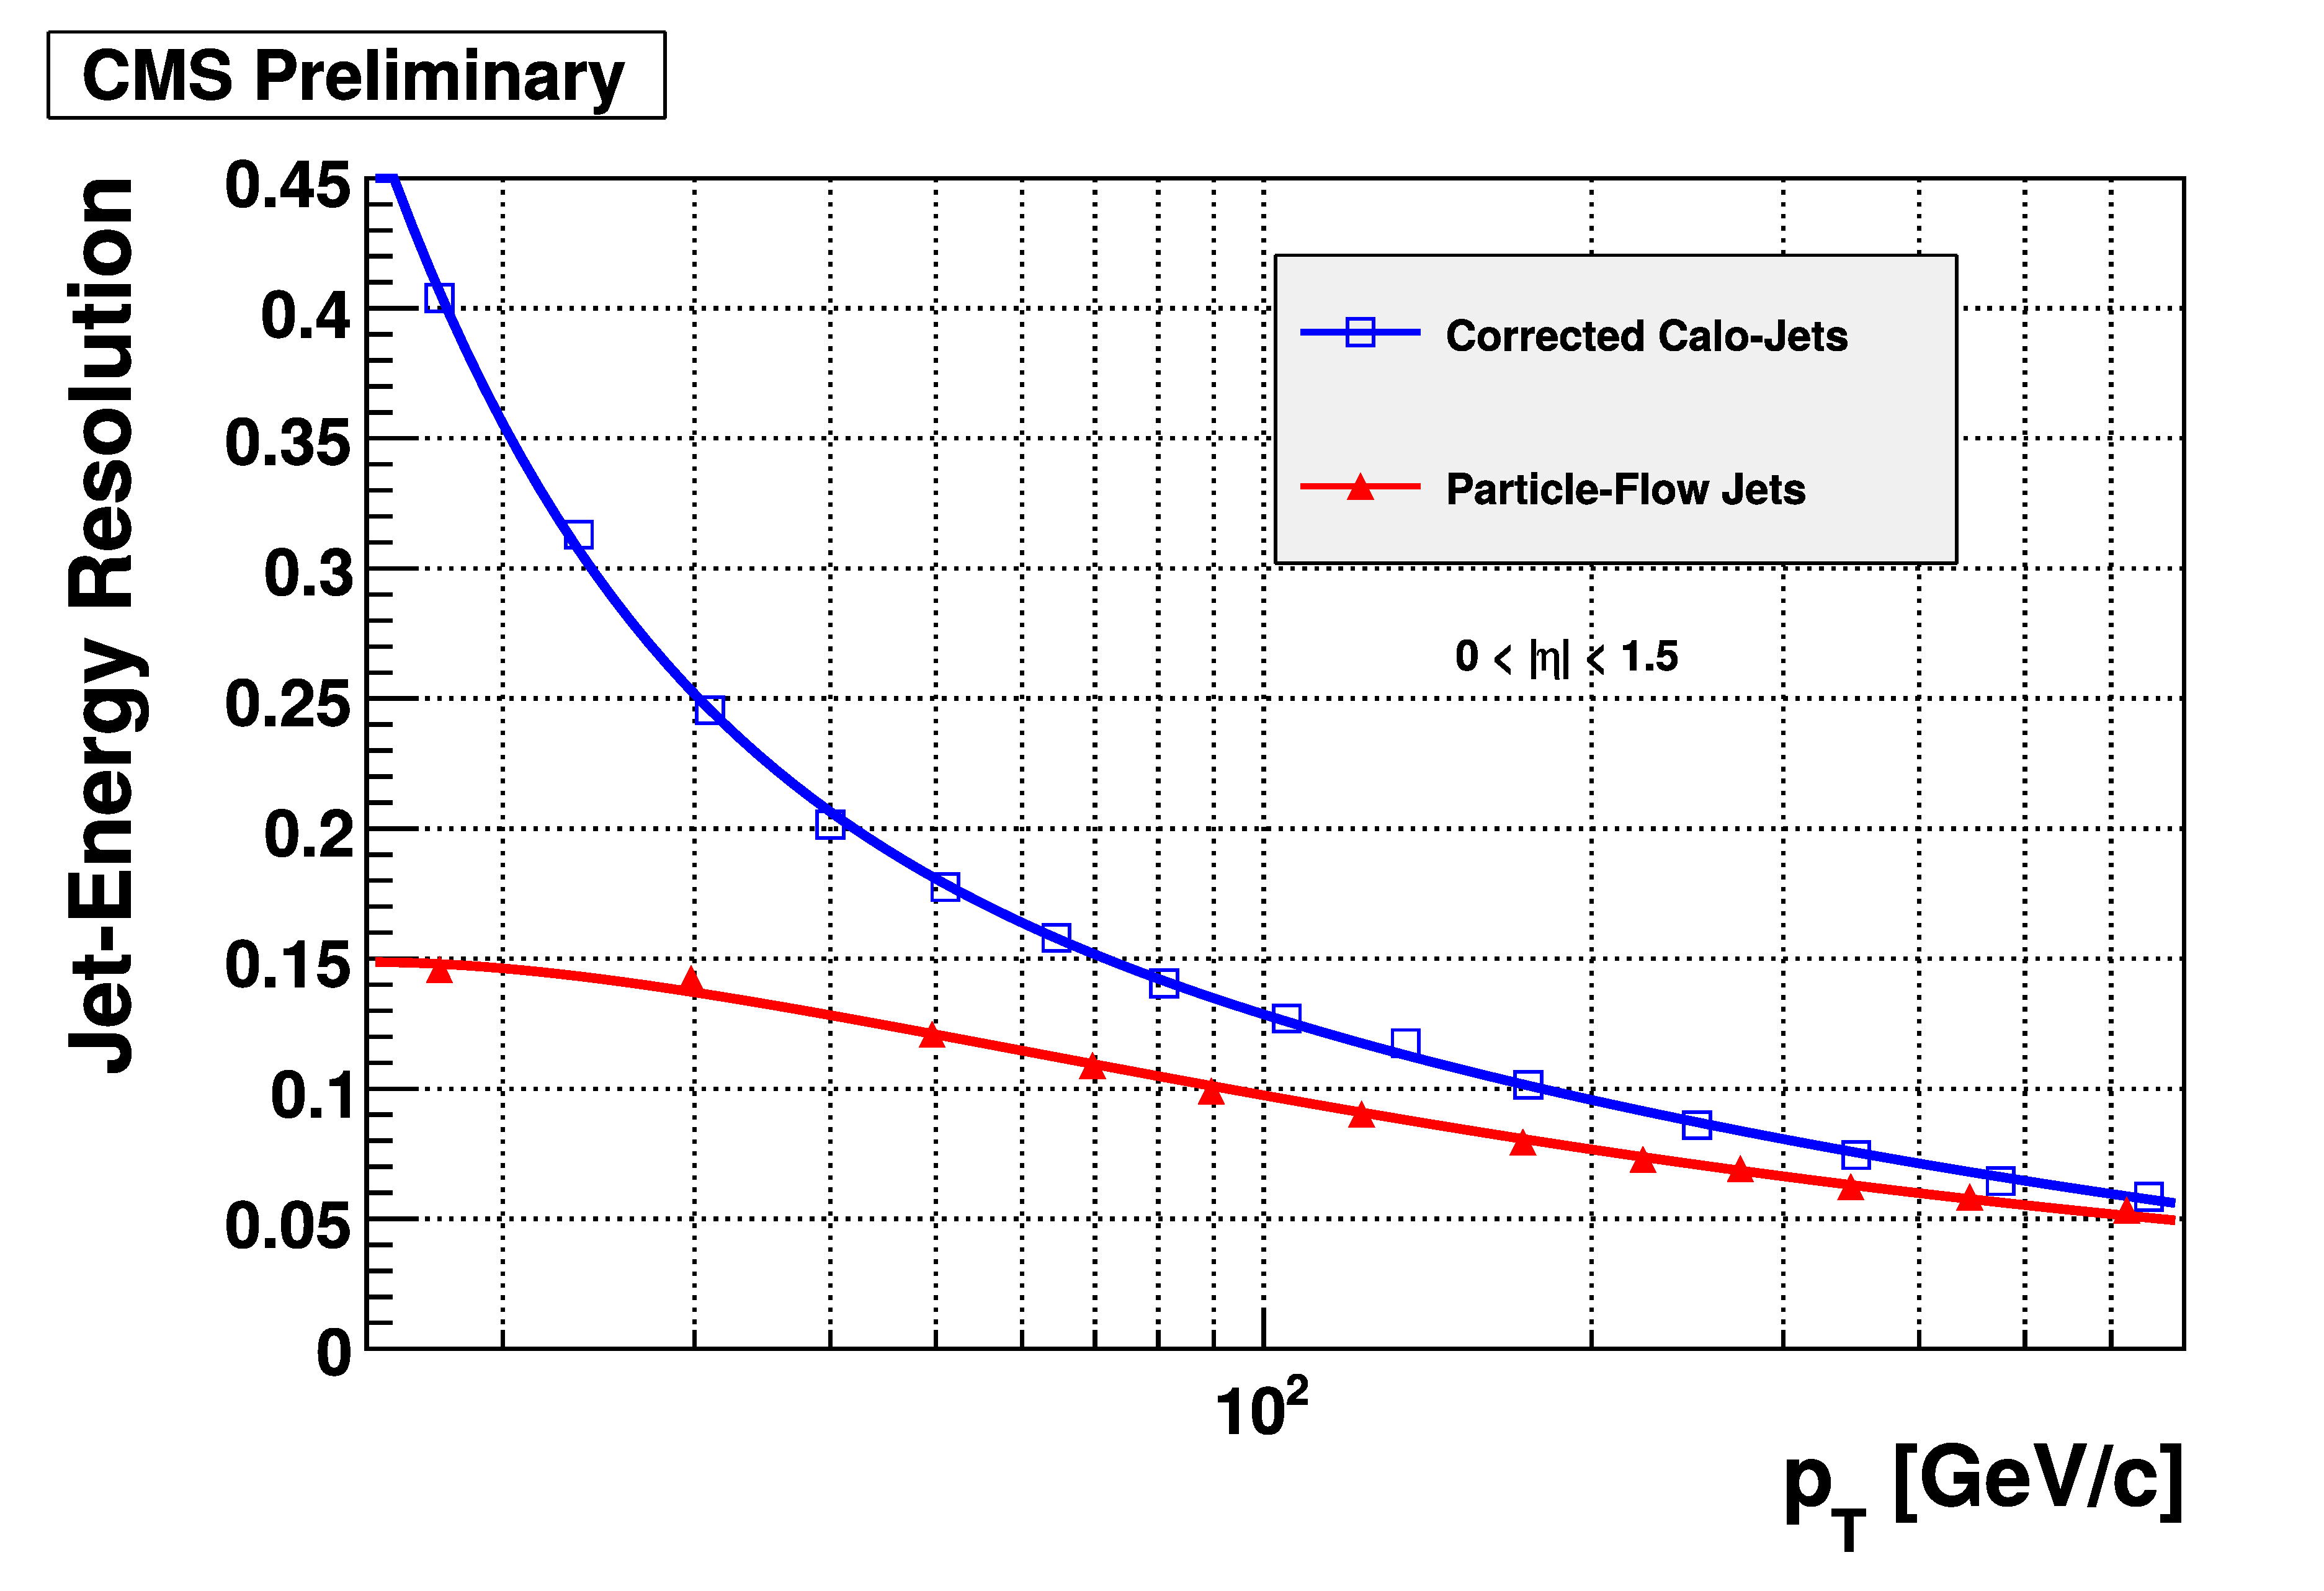
\includegraphics[width=0.45\textwidth]{chapitre3/figs/pf_vs_calo_jets.pdf}} \hfill
    \subcaptionbox{\label{fig:pf_jets_composition}}[0.45\textwidth]{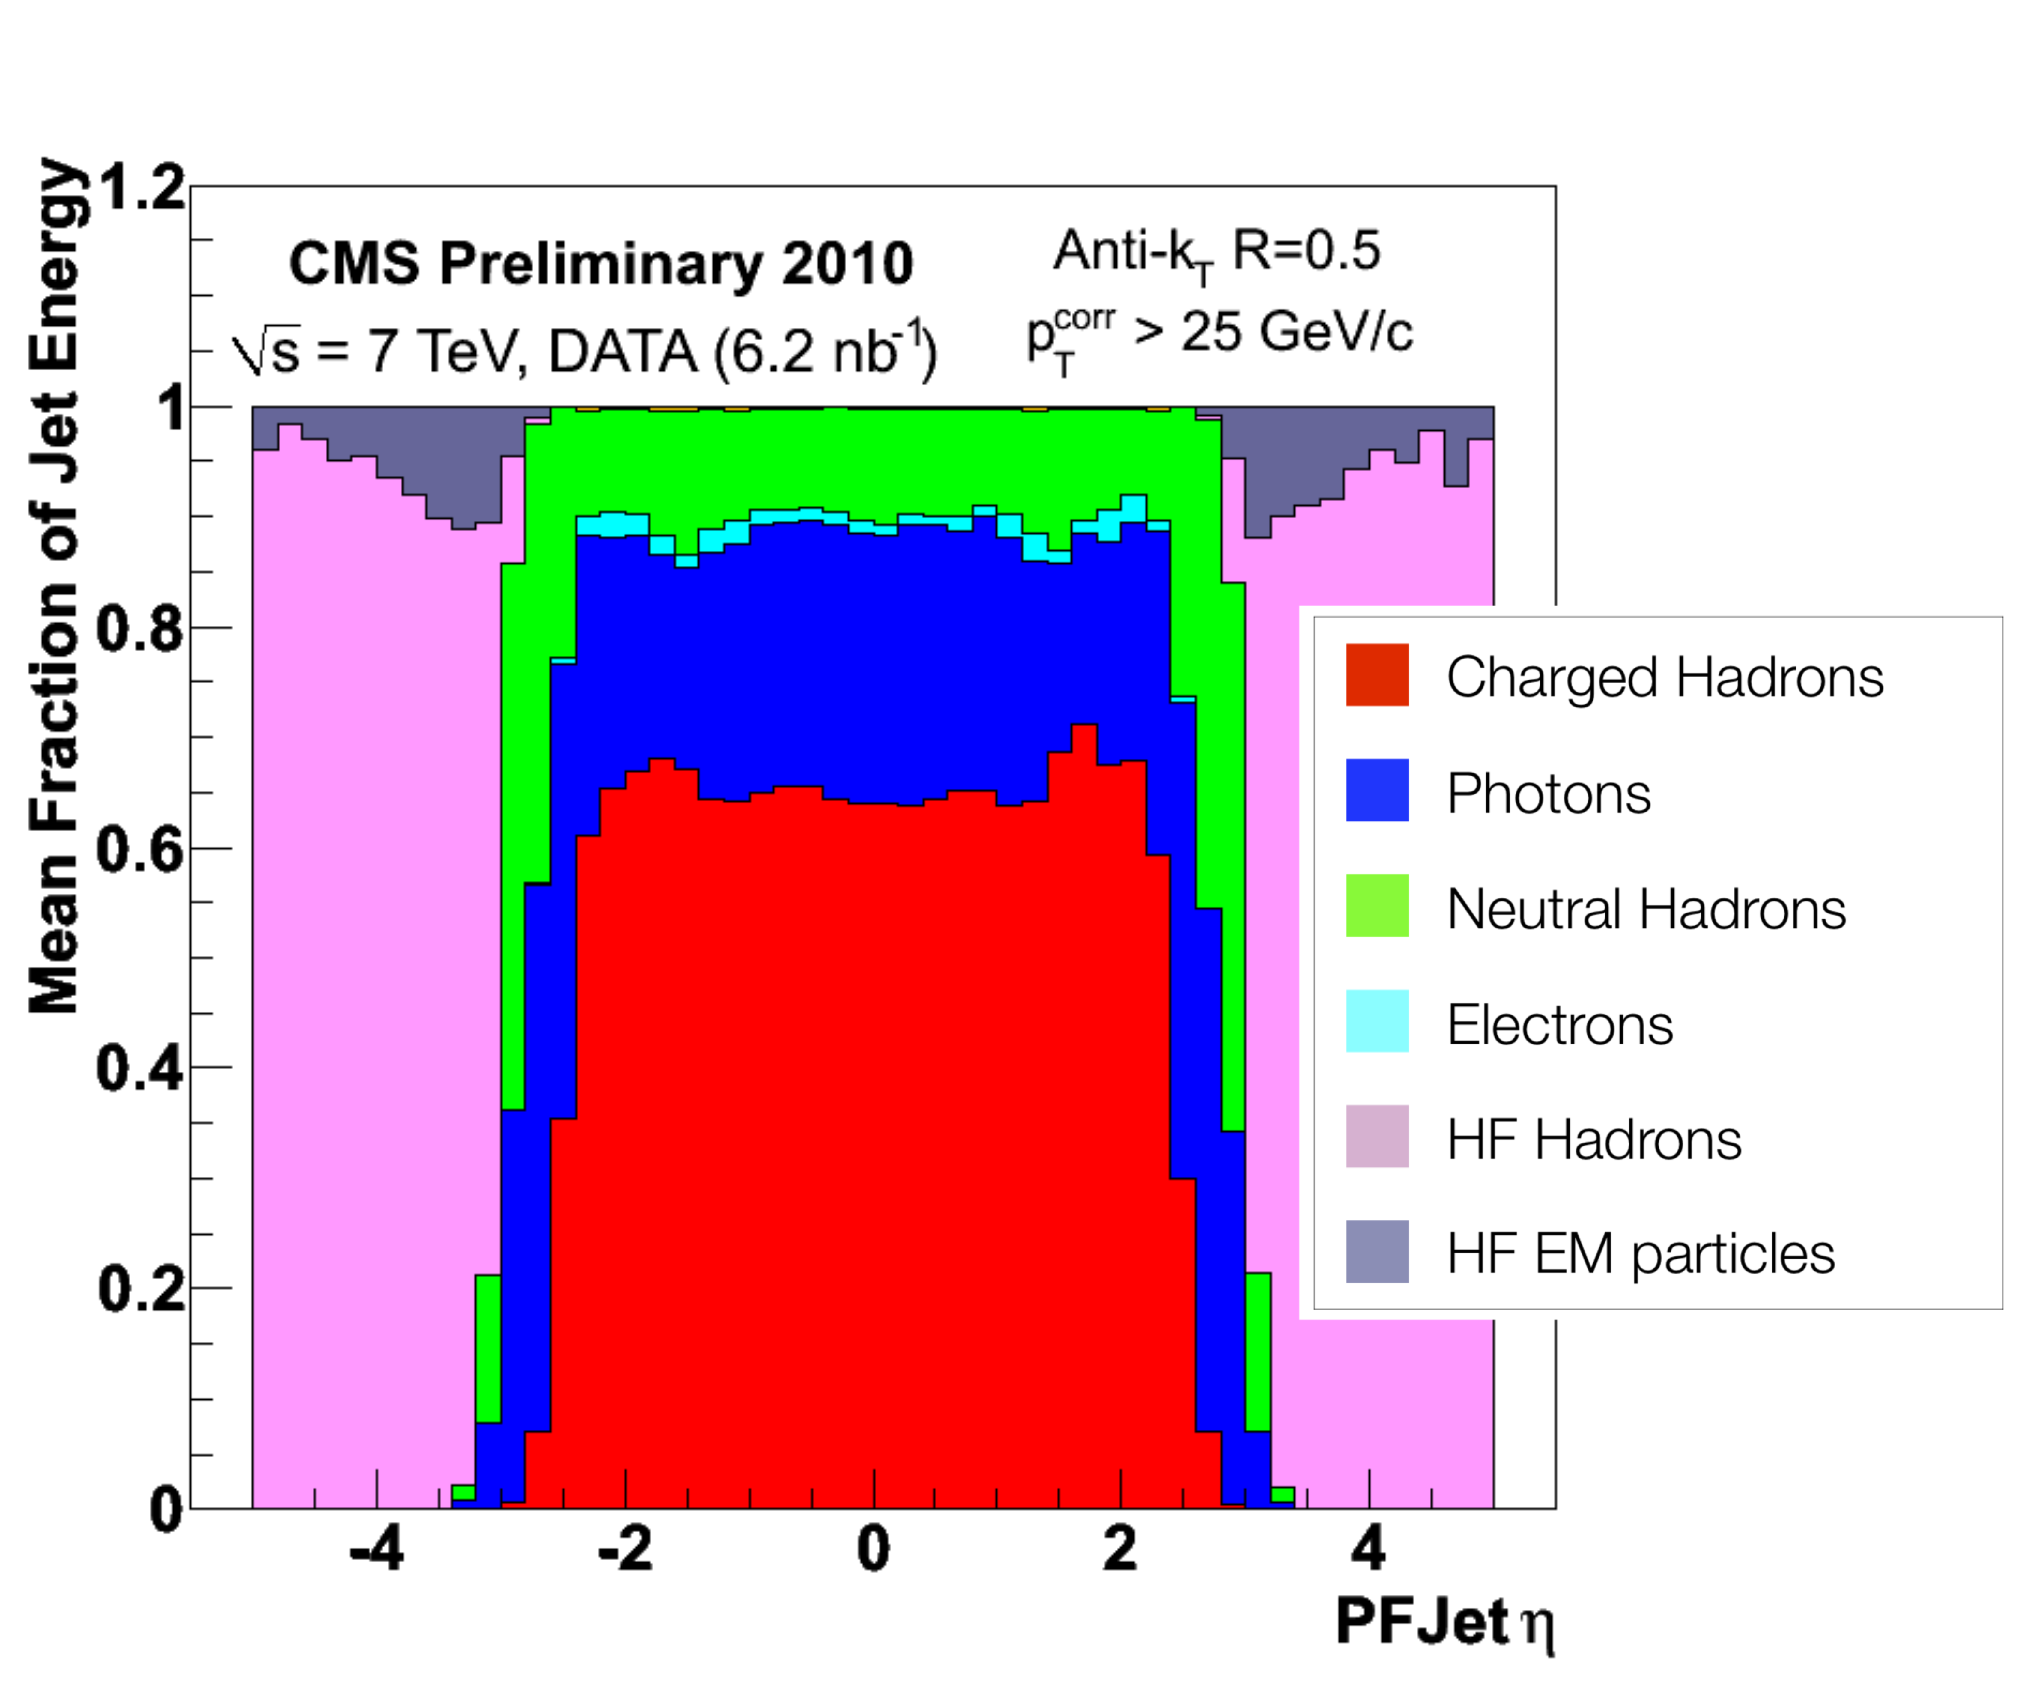
\includegraphics[width=0.45\textwidth]{chapitre3/figs/pf_jets_composition.png}}
    \caption{(\subref{fig:pf_vs_calo_jets_reso}) Résolution sur la reconstruction des jets \emph{particle-flow} (rouge) et calorimétriques (bleu) et (\subref{fig:pf_jets_composition}) composition énergétique des jets \emph{particle-flow}. La proportion de hadrons chargés chute brutalement à partir de $\abs{\eta} > 2.4$, puisque le trajectographe n'est plus disponible pour les identifier \citep{cms_pf_jets}.}
    \label{fig:pf_jets_perf}
\end{figure}

\subsubsection{Correction de l'énergie des jets}

L'énergie des jets reconstruits nécessite d'être calibrée pour plusieurs raisons. Premièrement, il arrive que des particules créées lors de l'hadronisation ne soient pas correctement agglomérées dans le jet, souvent parce que la trajectoire de ces particules dévie trop de la trajectoire initiale du quark. Enfin, des problèmes de calibrations des sous-détecteurs viennent aussi dégrader la mesure de l'énergie des jets.

La calibration des jets est effectuée en différentes étapes, présentées en détails dans le \cref{chap:jetmet}.

\subsubsection{L'algorithme d'identification des jets de $b$} \label{sec:b_tagging}

\begin{figure}[tbp]
    \centering
    \subcaptionbox{\label{fig:btag_discri}}[0.45\textwidth]{\includegraphics[width=0.45\textwidth]{chapitre3/figs/btag_tt_csv.pdf}} \hfill
    \subcaptionbox{\label{fig:btag_csv_eff}}[0.45\textwidth]{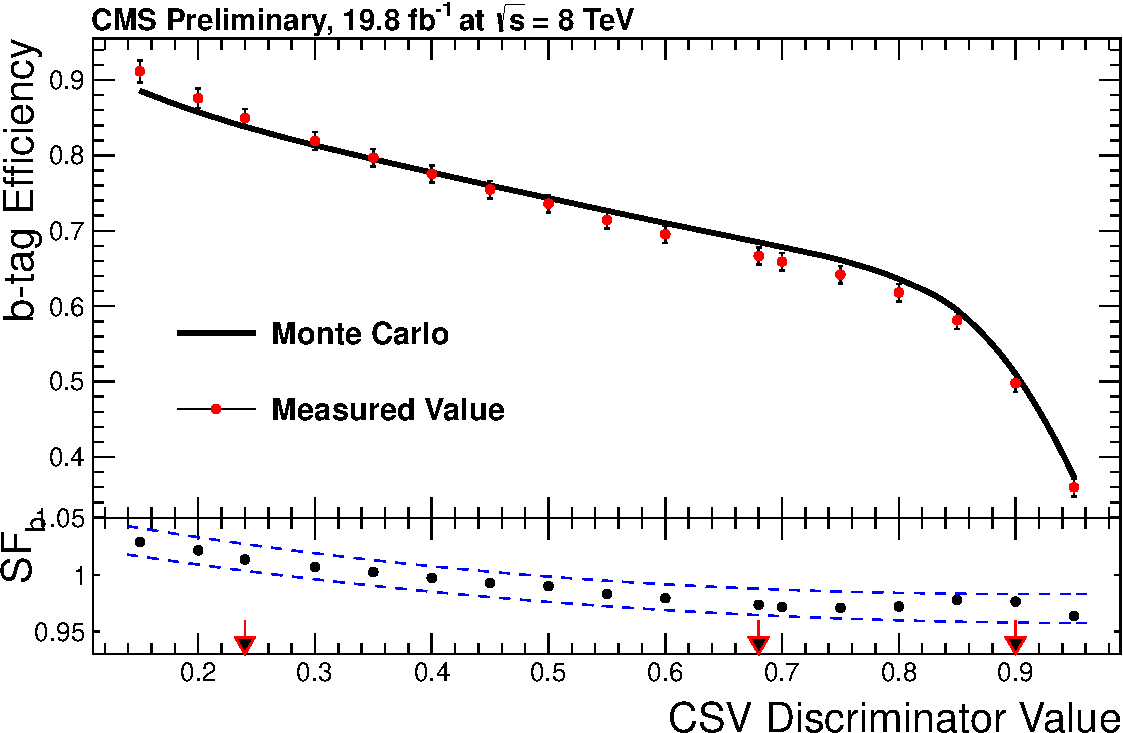
\includegraphics[width=0.45\textwidth]{chapitre3/figs/btag_csv_eff.pdf}}
    \caption{(\subref{fig:btag_discri}) Sortie de l'analyse multivariée de l'algorithme CSV sur un échantillon enrichi \ttbar. Les hautes valeurs sont enrichies en quark $b$, et les trois flèches correspondent aux points de fonctionnements (lâche, moyen, et dur) défini par la collaboration. (\subref{fig:btag_csv_eff}) Efficacité d'étiqueter un jet de $b$ en fonction de la valeur du discriminant. Un point de fonctionnement lâche est plus efficace, mais étiquette aussi plus souvent d'autres jets comme jets de $b$ \citep{btag_perf}.}
    \label{fig:btag_perf}
\end{figure}


Les propriétés des hadrons $B$ peuvent être utilisées pour identifier les jets qu'ils forment. Ces propriétés incluent, entre autre, leur grande masse et leur grand temps de vie. Plusieurs algorithmes sont disponibles dans CMS permettant d'identifier les jets formés par un quark $b$ (\emph{b-tagging}, pour étiquetage des $b$), chacun exploitant une spécificité des hadrons $B$. L'algorithme actuellement utilisé par la collaboration CMS est l'algorithme \emph{Combined Secondary Vertex} (CSV, vertex secondaire combiné), qui est une combinaison de plusieurs algorithmes.

Cet algorithme exploite toutes les variables connues pour discriminer les jets de $b$, telles que des informations sur des vertex déplacés, la cinématique du jet, etc. Une analyse multivariée (MVA) permet ensuite de fournir un discriminant, et trois points de fonctionnement sont définis, chacun augmentant l'efficacité de correctement étiqueter un jet de $b$, mais au détriment d'un taux de faux plus important (voir \cref{fig:btag_perf}). Pour le point de fonctionnement moyen, l'efficacité de bien étiqueter un jet de $b$ est \tilde\SI{70}{\%}, tandis que la probabilité d'étiqueter comme $b$ un jet d'une autre saveur est \tilde{1}{\%}.

\subsection{L'énergie transverse manquante} \label{sec:met}

\begin{figure}[tbp]
    \centering
    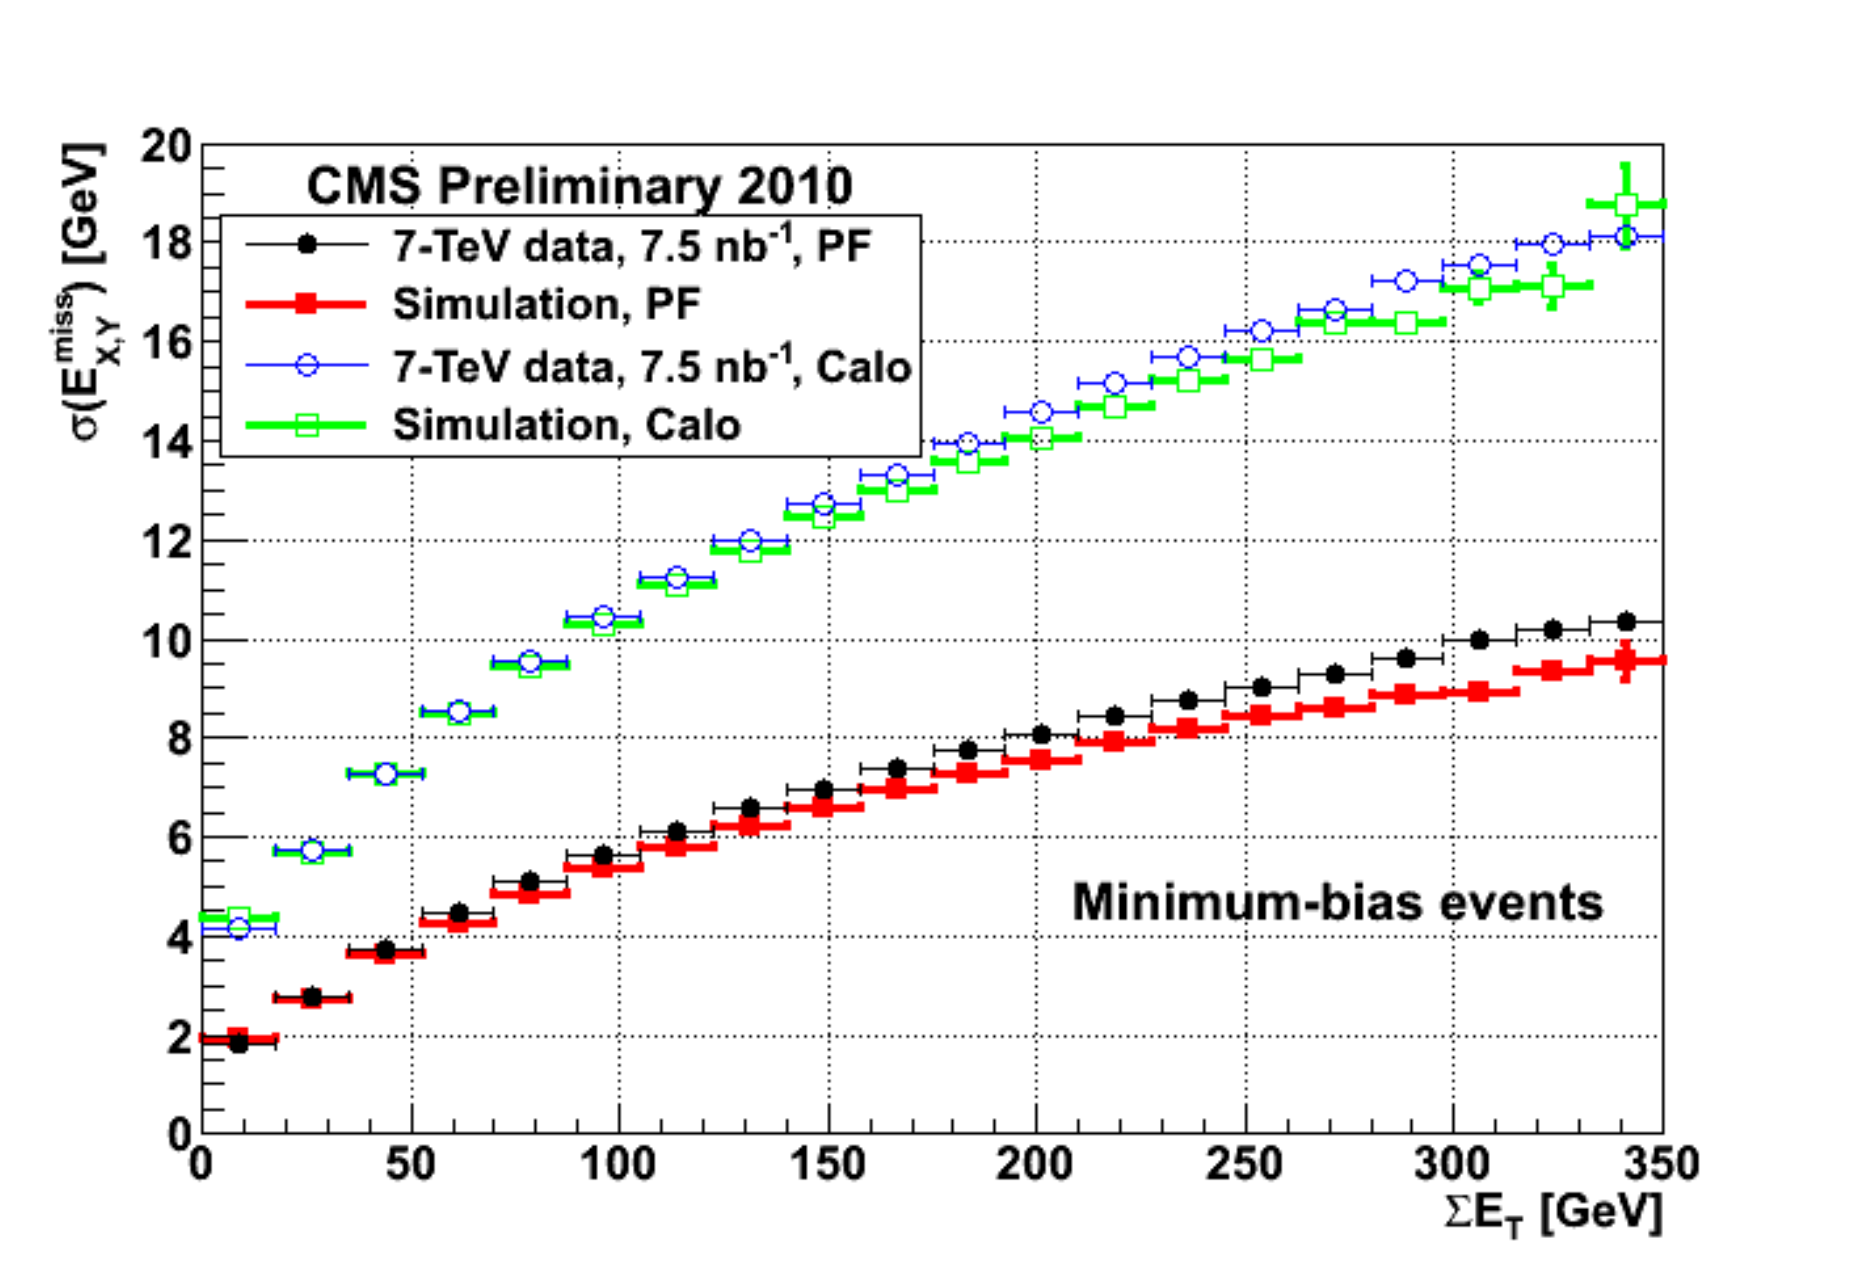
\includegraphics[width=0.7\textwidth]{chapitre3/figs/pf_met_resolution.png}
    \caption{Résolution de l'énergie transverse manquante \emph{particle-flow} et calorimétrique en fonction de la somme scalaire de l'énergie transverse de toutes les particules dans l'événement ($\sum E_T$), obtenue sur les données 2010. \citep{cms_pf_jets}.}
    \label{fig:met_resolution}
\end{figure}

Par définition, les collisions au sein de CMS se déroulent le long de l'axe $z$. L'impulsion dans le plan ($x$, $y$) est donc nulle. Par conservation de l'impulsion, ce bilan doit rester nul après reconstruction de l'événement : un bilan non nul signifie que des particules n'ont pas été correctement reconstruites. C'est par exemple le cas des neutrinos, qui n'interagissent que très peu avec la matière, et ne sont par conséquent jamais détectés.

Afin de quantifier cette perte d'énergie, on introduit le vecteur énergie transverse manquante. La norme de ce vecteur est communément appelée énergie transverse manquante (MET), symbolisée par \met. A l'aide de l'algorithme de \emph{particle-flow}, on définit le vecteur énergie transverse manquante comme l'opposé de la somme vectorielle des impulsions transverses de toutes les particules de l'événement. La résolution sur la mesure de \met est très importante, puisque de nombreux modèles de nouvelle physique prédisent des particules qui interagissent peu voire pas avec la matière : l'énergie manquante est alors le seul moyen de pouvoir les mettre en évidence. On présente \cref{fig:met_resolution} la résolution de \met reconstruite grâce au \emph{particle-flow}, obtenue sur les données 2010. À titre de comparaison, la résolution de \met reconstruite seulement à l'aide des dépôts calorimétriques (calomet) est aussi présentée dans la même figure.

\section{Conclusion}

On a pu voir au cours de ce chapitre combien il est important de posséder une chaine de simulation complète et performante. Dans un premier temps, il faut être capable de générer correctement un processus physique. Cette étape est réalisée par les générateurs d'événements à éléments de matrice, ainsi que par les générateurs à gerbe partonique. Il est ensuite nécessaire de simuler de façon précise la réponse du détecteur. Cette étape est cruciale, et impose une excellente connaissance du détecteur : des progrès sont continuellement réalisés afin d'améliorer la simulation. Enfin, le processus de reconstruction des objets physiques, commun à la simulation et aux données collectées, est capital pour les analyses de physique. CMS dispose de puissants outils de reconstruction. À l'aide de l'algorithme du \pf, tous les sous-détecteurs sont utilisés pour la reconstruction des objets physiques, ce qui permet d'améliorer sensiblement la résolution des objets reconstruits. On dispose également d'algorithmes performants pour la reconstruction des jets, primordial dans un environnement hadronique où un grand nombre de jets sont produits.

\medskip

Le prochain chapitre est dédié aux corrections en énergie appliquées aux jets, en insistant particulièrement sur le dernier niveau de correction, qui fût l'un des travaux que j'ai effectué durant ma thèse.